%%%% Modèle proposé par kira.ribeiro@universite-paris-saclay.fr  %%%%
%%%% màj : 27/01/2023 %%%%

\documentclass{maThese}

\begin{document}
\begin{titlepage}

%\thispagestyle{empty}

\newgeometry{left=6cm,bottom=2cm, top=1cm, right=1cm}

\tikz[remember picture,overlay] \node[opacity=1,inner sep=0pt] at (-13mm,-135mm){\includegraphics{Frame-ups.pdf}};

%*****************************************************
%******** NUMÉRO D'ORDRE DE LA THÈSE À COMPLÉTER *****
%******** POUR LE SECOND DÉPOT                   *****
%*****************************************************

\color{white}

\begin{picture}(0,0)
\put(-152,-743){\rotatebox{90}{\Large \textsc{THESE DE DOCTORAT}}} \\
\put(-120,-743){\rotatebox{90}{NNT : 2020UPASA001}}
\end{picture}
 
%*****************************************************
%******************** TITRE **************************
%*****************************************************

\flushright
\vspace{10mm} % à régler éventuellement
\color{Prune}

\fontsize{22}{26}\selectfont
  \Huge Méthodes d’analyse comparée des pangénomes procaryotes : \\ explorer la diversité génomique inter-espèces pour une meilleure  compréhension du métabolisme \\

\normalsize
\color{black}
\Large{\textit{Methods for comparative analysis of prokaryotic pangenomes: exploring interspecies genomic diversity for a better understanding of metabolism}} \\
%*****************************************************


\fontsize{8}{12}\selectfont

\vspace{1.5cm}

\normalsize
\textbf{Thèse de doctorat de l'université Paris-Saclay} \\

\vspace{6mm}

\small École doctorale n$^{\circ}$ 577, STRUCTURE ET DYNAMIQUE DES SYSTÈMES VIVANTS (SDSV)\\
\small Spécialité de doctorat : Sciences de la vie et de la santé\\
\small Graduate School : Life Sciences and Health. Référent : Université d’Évry Val d’Essonne \\
\vspace{6mm}

\footnotesize Thèse préparée dans la (ou les) unité(s) de recherche \textbf{Université Paris-Saclay, Univ Evry, CNRS, CEA, Génomique métabolique, 91057, Evry-Courcouronnes, France.}, sous la direction de \textbf{David Vallenet}, Directeur de recherche CEA, Genoscope CEA, la co-direction de \textbf{Alexandra Calteau}, Chercheure CEA, Genoscope CEA\\
\vspace{15mm}

\textbf{Thèse soutenue à Paris-Saclay, le 19 mai 2025, par}\\
\bigskip
\Large {\color{Prune} \textbf{Jérôme ARNOUX}} % Changer le Prénom et le NOM

%************************************
\vspace{\fill} % ALIGNER LE TABLEAU EN BAS DE PAGE
%************************************

\bigskip

\flushleft
\small {\color{Prune} \textbf{Composition du jury}}\\
{\color{Prune} \scriptsize {Membres du jury avec voix délibérative}} \\
\vspace{2mm}
\scriptsize
\begin{tabular}{|p{7cm}l}
\arrayrulecolor{Prune}
\textbf{Lucie BITTNER} &  Rapportrice \\ 
Maîtresse de conférence, Sorbonne Université   &   \\ 
\textbf{François Sabot} &  Rapporteur \\ 
Directeur de recherche, université de Montpellier  &   \\ 
\textbf{Stéphanie BURY-MONÉ} & Examinatrice\\ 
Professeure, Université Paris Saclay & \\
\textbf{Jean CURY} &  Examinateur \\ 
Chercheur, Institut Pasteur   &   \\
\end{tabular} 
\vspace{2mm}

\begin{tabular}{p{7cm}l}
\textbf{Alexandra CALTEAU} & Invitée\\ 
Chercheuse, CEA & \\
\textbf{David Vallenet} & Invité\\ 
Directeur de recherche, CEA & \\
\end{tabular} 

\end{titlepage}
\newpage
\thispagestyle{empty}
\mbox{}
\newpage
\thispagestyle{empty}
\mbox{}
\newpage
\thispagestyle{empty}
\mbox{}
\newpage

\newgeometry{top=4cm, bottom=4cm, left=2cm, right=2cm}

\newgeometry{margin=1in} % Ajustez les marges selon vos besoins
\thispagestyle{empty} % Supprime les en-têtes et pieds de page
\vspace*{\fill} % Espace vertical flexible pour centrer verticalement
\begin{flushright}
    \begin{minipage}{0.7\textwidth} % Ajustez la largeur selon vos besoins
        À ma femme Helen et notre petite fille à naitre. \\
        
        \vspace{6pt}
        
        À ma grand-mère Bernadette, qui a toujours été un modèle et une femme que j'admire. \\
        
        \vspace{6pt}
        
        À l'espoir que les hommes comprennent que détruire la nature, c'est se détruire nous-même : "Actuellement, l'homme mène une guerre contre la nature. S'il gagne, il est perdu." - Hubert Reeves \\
        
        \vspace{6pt}
        
        Aux générations futures : "Nous n'héritons pas de la terre de nos ancêtres, nous l'empruntons à nos enfants." - Antoine de Saint-Exupéry
    \end{minipage}
\end{flushright}
\vspace*{\fill}
\restoregeometry % Restaure les marges originales

\thispagestyle{empty}
\mbox{}
\newpage
\renewcommand{\thepage}{\Roman{page}}
\setcounter{page}{1}

\tableofcontents

\newgeometry{top=4cm, bottom=4cm, left=4cm, right=4cm}

\listoffigures

\newgeometry{top=4cm, bottom=4cm, left=4cm, right=4cm}

\listoftables

%\thispagestyle{titleFoot}
% \addcontentsline{toc}{chapter}{Acronymes}
% \printacronyms[title = \centering Acronymes]
% \newpage

\newgeometry{top=4cm, bottom=4cm, left=4cm, right=4cm}

% \newgeometry{top=4cm, bottom=4cm, left=2cm, right=2cm}
% \addcontentsline{toc}{chapter}{Acronymes}
% \printacronyms[title = \centering Acronymes]

% \newgeometry{top=4cm, bottom=4cm, left=4cm, right=4cm}

% \newgeometry{top=4cm, bottom=4cm, left=2cm, right=2cm}

% \addcontentsline{toc}{chapter}{Glossaire}
% \printglossary

% \newgeometry{top=4cm, bottom=4cm, left=4cm, right=4cm}
% \newacronym{Test}{Test}{TTTT EEEE SSS TTT}
% \gls{Test}
\newgeometry{left=2.5cm,right=2.5cm,top=1.5cm, bottom=2.5cm, centering}
\chapter*{Remerciements}
\addcontentsline{toc}{chapter}{Remerciements}

Je commencerai par remercier toutes les personnes qui ont contribué de près ou de loin à la conclusion de ce chapitre de ma vie. La thèse de doctorat est une expérience unique, que j'ai pu vivre en y prenant beaucoup de plaisir. Je retiendrai de ces années que le monde de la recherche est un monde vivant et dynamique, où chaque personne contribue à la réussite et au progrès collectif. À toutes les personnes qui ne verraient pas leurs noms cités, veuillez m'excuser par avance et sachez que je garde en mémoire toutes les personnes qui ont pu me soutenir ces dernières années.

Je me dois d'abord (mais je le fais bien volontiers) de remercier David Vallenet, directeur du LABGeM et directeur de ma thèse. Merci de m'avoir fait confiance pour mener à bien ces projets de recherches. J'ai beaucoup appris à tes côtés, sur le plan technique, mais aussi sur les rouages du monde académique. Je me souviendrai particulièrement de ma première conférence internationale à FEMS où tu m'as accompagné.

Je remercie aussi Alexandra Calteau, chercheuse au LABGeM et co-directrice de ma thèse. Au-delà de toutes les connaissances biologiques et bioinformatiques que tu m'as partagées, je garderai l'image d'une personne extrêmement humaine qui a su me présenter des opportunités pour me former à devenir un chercheur dans tous ces aspects. Tu as su être plus que compréhensive sur des événements personnels qui ont certainement impacté ma thèse et pour ça je te remercie énormément.

Merci à Jean Mainguy, tu as été d'une aide plus que bienvenue pendant tous mes travaux de thèse. Je pense sincèrement que tu as abattu le travail de plusieurs personnes à toi tout seul et sans ça je ne sais pas si les outils de pangénomique du LABGeM seraient dans leur état actuel. 

À Adelme Bazin et Guillaume Gautreau, je vous remercie de ne pas avoir quitté le bateau après votre thèse et d'être restés disponibles pour mes questions et pour tout le travail que nous avons pu accomplir sur PPanGGOLiN. Je vous tiens en haute estime, vous m'impressionnez toujours par vos connaissances, vos compétences et aussi par votre sympathie.

Pour Laura Bry et Quentin Fernandez De Grado, j'espère avoir su être un bon encadrant et que vous gardiez un bon souvenir de votre passage au LABGeM. Sachez que j'ai aussi beaucoup appris à vos côtés. Je vous souhaite toute la réussite possible pour votre avenir et j'espère vous croiser à l'occasion.

À Eddy Élisée, merci pour ta joie de vivre et pour avoir été toujours été le premier arrivé au laboratoire pour prendre le premier café. Tu es une personne rayonnante avec qui on aimerait travailler plus souvent ou même juste faire tourner quelques molécules.

Alexandre Protat, tu restes un membre honoraire du LABGeM. Merci d'avoir organisé tous ces GenoPub, et merci pour toutes ces discussions politiques où même si nos opinions étaient parfois opposées, nous avons pu parler sans amertume.

Merci à tous les autres membres du LABGeM. David Roche pour ta sympathie, ton calme et ta bienveillance. Stéphanie Fouteau, pour ton sourire et ta gentillesse. Zoé Rouy, pour tes conseils et ton savoir. Aurélie Génin-Lajus, pour ton énergie à revendre. Marc Stam, pour nos discussions autour du café. À tous les membres passés et présents, encore merci.

Je remercie également les membres de mon comité de suivi : Hélène Chiapello, Sophie Abby et Vincent Lacroix. Vous avez été de précieux conseils et vous avez toujours jugé mon travail avec honnêteté et bienveillance. J'espère que le résultat final sera à la hauteur des promesses et que nous pourrons nous revoir à l'occasion.

Je remercie tous mes amis qui m'ont supporté pendant ces 3 dernières années. Merci à Maud Repellin pour avoir été présente lorsque j'en avais besoin. Merci à Chloé Beaumont, Florian Jeanneret et Alba Caparros-Roissard pour nos moments de partage d'expérience de doctorant.

Merci à tous les membres de ma famille qui ont su me soutenir, chacun à leur manière. Merci à mon frère et ma s\oe ur qui, même si mes travaux de recherches ne les passionnaient pas, ont bien essayé de me supporter. Merci à mes parents, d'avoir cru en moi et de m'avoir permis de saisir les opportunités qui se présentaient à moi. Merci à mes grands-parents pour leur soutien moral dans toutes les difficultés.

Pour terminer, je ne peux que remercier ma femme Helen qui a toujours été présente pour me soutenir dans toutes les difficultés que j'ai pu rencontrer pendant ma thèse. Même si ce n'était pas toujours évident de comprendre pourquoi j'ai choisi ce métier et cette voie, tu as toujours pensé d'abord à moi et à mon bonheur. Au moment où j'écris ces lignes, tu me prépares le plus beau des cadeaux et je n'ai pas les mots pour t'exprimer ma reconnaissance.

Merci bien sûr à vous, lecteur de ce manuscrit de thèse, j'espère que celui-ci sera à la hauteur de vos attentes.
\newpage
\renewcommand{\thepage}{\arabic{page}}
\setcounter{page}{1}
\chapter*{Introduction}
\addcontentsline{toc}{chapter}{Introduction}

Cette introduction a pour objectif de faire le panorama scientifique et historique des différents sujets qui seront abordés dans ce manuscrit de thèse. Elle fait aussi office d'entrée en matière pour les personnes non expertes qui liront ce manuscrit. Pour ces quelques lignes, je me permettrai donc quelques facilités et imprécisions scientifiques.%, en espérant qu'elles me seront excusées.


Les conditions qui ont permis à la vie de naître sur Terre suscitent encore de nombreuses questions et sont à l'origine de débat scientifique passionnant. Néanmoins, les premières traces de vie retrouvées remontent à 4 milliards d'années et correspondent à des microorganismes, des êtres invisibles à l'{\oe}il nu. Ces microorganismes colonisent la Terre depuis des milliards d'années et représentent aujourd'hui la proportion d'êtres vivants la plus importante en termes de nombre et de diversité. Ils jouent un rôle crucial dans les écosystèmes, les cycles biogéochimiques et la santé de la planète comme de la nôtre. En effet, ces microbes sont connus pour poser des problèmes de santé publique (épidémie, hygiène\dots), de contamination des plantes et des sols, ou encore de dégradation des matériaux. En contrepartie, ils peuvent aussi améliorer notre santé (les probiotiques par exemple), fertiliser les sols et épurer les eaux et être utile dans l'industrie et les biotechnologies (fermentation des fromages et des bières). Pourtant, la microbiologie, l'étude des microorganismes, reste une science relativement récente. Même s'il existe bien, dans l'Antiquité, certains savants et philosophes qui avaient déjà imaginé ces "animaux invisibles", marquant une compréhension primitive de la transmission des maladies infectieuses, il faudra attendre l'invention du microscope par Leeuwenhoek, au XVIIe siècle, pour qu'il fasse les premières observations d'\textit{animaculum}, marquant la naissance de la microbiologie. La microbiologie du XVIIe au XXe siècle a amené de grandes découvertes et révolution scientifique, notamment en médecine. Nous pouvons citer les travaux de Louis Pasteur qui a prouvé, en 1877, que les maladies infectieuses étaient causées par des microorganismes (staphylocoque, pneumocoque et streptocoque), ou encore d'Alexander Fleming qui découvrit, en 1928, la pénicilline, le premier agent antibiotique. 


En s'éloignant quelque peu de la microbiologie, toujours entre le XVIIe et XXe siècle, les chimistes s'intéressent aux molécules du vivant. Autour des années 1800, Le Français Antoine Fourcroy va faire la première description de substances azotées dans les organismes vivants, qu'il appelait "substances animales". C'est ensuite, en 1835, que le chimiste néerlandais Gérardus Johannes Mulder découvre des chaînes de substance azotées, qui seront introduites sous le terme de protéine par le chimiste suédois Jöns Jacob Berzelius en 1838. Le mot vient du grec \textit{proteios}, qui signifie "de première importance", soulignant l'intérêt fondamentale de ces molécules composées de carbone, hydrogène, azote et oxygène, avec des proportions spécifiques, dans les organismes vivants. Enfin, en 1894, le chimiste allemand, Emil Fischer, démontra que les protéines sont composées d'acides aminés, unité de base des protéines, liés par des liaisons peptidiques. Il déterminera la composition et la structure de plusieurs d'entre eux. La fin du XIXe siècle voit aussi la découverte d'une autre molécule du vivant, l'acide désoxyribonucléique, mieux connue sous l'acronyme ADN. C'est le biologiste suisse Friedrich Miescher qui découvre, en 1869, une substance riche en phosphore dans les cellules du pus, qu'il appelle "nucléine". Il faudra attendre près d'un demi-siècle (1929) pour que Phoebus Levene, biochimiste russe-américain, identifie les composants de base de l'ADN : les nucléotides. Plus tard, en pleine Seconde Guerre mondiale, les chercheurs Oswald Avery, Colin MacLeod et Maclyn McCarty, confirment l'hypothèse de Miescher, en montrent que l’ADN est la substance qui transfère les caractères héréditaires et que l'ADN est le support de l’information génétique. Pour terminer, les travaux de James Watson, Francis Crick  et Rosalind Franklin, ont permis de décrire la structure de la molécule d'ADN. Toutes ces découvertes ont ouvert la voie à de nombreuses autres dans tous les domaines : médecine, agro-alimentaire, biotechnologie, et sont le socle de la génétique moderne.

Les développements technologiques de la seconde moitié du XXe siècle, et notamment l'apparition du séquençage et de l'informatique, amènent les chercheurs à créer une nouvelle discipline pour l'étude de la structure et de la composition des molécules du vivant : la bioinformatique. En 1955, Frederick Sanger séquencera la première protéine, l'insuline. Cette découverte, récompensée par un prix Nobel, a établi la base du séquençage. Peu de temps après, Margaret Dayhoff, une pionnière de la bioinformatique, développe l'un des premiers programmes informatiques pour analyser les séquences de protéines. Elle publiera d'ailleurs, en 1969, le premier atlas de séquences protéiques, jetant les bases de l'analyse des séquences biologiques. À partir de là, la bioinformatique ne cessera d'évoluer avec les techniques de séquençage. En 1970, Saul Needleman et Christian Wunsch introduisent un algorithme pour l'alignement global des séquences, qui est toujours utilisé aujourd'hui. En 1977, Sanger va à nouveau révolutionner le domaine de la biochimie en proposant une méthode de séquençage de l'ADN qui portera son nom. Elle devient rapidement la méthode de référence en raison de sa précision. Dans les années 80, la méthode s'automatise, devient plus rapide et précise. On voit alors se développer les premières bases de données accessibles au public pour stocker des séquences génétiques et protéiques. En 1990, est lancé le Projet du Génome Humain (HGP), un effort international visant à séquencer l'intégralité du génome humain. Ce projet catalyse de nombreux développements en bioinformatique, notamment dans la gestion et l'analyse des grandes quantités de données générées. Enfin, au début des années 2000, les technologies de séquençage sont de plus en plus performantes et abordables, faisant entrer la bioinformatique dans l'âge du \textit{Big Data}, la rendant essentielle dans de nombreux domaines d'étude en biologie.


La microbiologie et, pour ce qui va nous intéresser ici, l'étude de la génétique des microorganismes profitent de toutes ces nouvelles technologies pour développer ces connaissances. Elle va aussi subir cette explosion de la quantité d'informations disponible dans les bases de données. C'est pourquoi, microbiologistes et bioinformaticiens sont toujours à la recherche de nouvelles méthodes pour l'analyse de ces données. Alors que les programmes bioinformatiques s'attachaient à représenter et à étudier un génome en tant qu'une séquence indépendante des autres, un nouveau concept de représentation des génomes est apparu : le pangénome. Il permet de regrouper l'ensemble des génomes en une seule entité et donc rendre une représentation globale de l'ensemble de l'information contenue dans les génomes. Le pangénome garantit une meilleure représentation de la diversité des génomes, tout en étant plus adapté à l'analyse de grandes quantités de données. C'est dans ce cadre que j'ai effectué mon travail de thèse, avec pour objectif de proposer de nouvelles méthodes en pangénomique pour l'analyse comparé des génomes de microorganismes a l'ère du \textit{Big Data}.

%Cette courte introduction permet, je l'espère, de montrer le caractère multidisciplinaire et international de la bioinformatique, mais aussi de comprendre les bases sur lesquelles reposent nos connaissances.

Ce manuscrit sera divisé en plusieurs parties comme suit. Une première partie sera consacrée à contextualiser et à rendre compte des problématiques auxquelles répond ce travail de thèse. Dans cette partie, je donnerai la définition précise des termes que j'utiliserai et je reviendrai sur l'état de l'art en génomique comparée des procaryotes. Je poursuivrai par une seconde partie sur les développements méthodologiques que j'ai pu réaliser en pangénomique, notamment dans la suite logicielle PPanGGOLiN. La troisième partie sera consacrée au c{\oe}ur de mon sujet de thèse, c.-à-d., aux développements de méthodes pour la comparaison de pangénomes. Enfin, je présenterai une nouvelle approche utilisant les bases de données orientées graphe comme solution pour le stockage et l'étude des pangénomes. Pour terminer, je présenterai une discussion critique sur le travail réalisé pendant ces trois ans et demi. Je me dois également de rappeler aux lecteurs que la nature, \textit{mirabile dictu}, se distingue par une diversité extraordinaire, et que certaines règles ou affirmations généralement vérifiées peuvent souffrir d'exceptions.
\newline

Je vous souhaite bonne lecture de ce manuscrit, qui, je l'espère, fait preuve de toute la rigueur scientifique attendu et rend compte du travail réalisé pendant ces trois ans et demi de manière authentique.

\part{Procaryotes : de la biologie cellulaire à la génomique moderne}

Ce chapitre marque le début du manuscrit et posera les bases conceptuelles et méthodologiques, biologiques et bioinformatiques essentielles à la compréhension des travaux menés dans le cadre de cette thèse. Il s’agit ici de contextualiser les enjeux de la génomique des procaryotes et de la pangénomique, tout en abordant les principaux concepts et méthodes utilisés dans ce domaine.

Nous commencerons par un rapide retour sur ce qu'est un procaryote, un élément clé pour définir les bornes et le contexte d’application de nos recherches. Cette partie est essentielle pour comprendre les spécificités de ces organismes et leurs impacts sur les approches méthodologiques adoptées. Cette introduction permettra également de les situer dans la classification du vivant, notamment en revenant sur la structure cellulaire et l'organisation du génome, tout en apportant les éléments pour discuter de la notion d'espèce procaryote.

Une fois ce cadre biologique posé, nous aborderons les bases de la génomique comparée, en se focalisant sur l'application aux procaryotes. Ce moment sera l’occasion de clarifier l’utilisation de simplifications ou de choix algorithmiques, souvent nécessaires en raison des caractéristiques propres à ces génomes. Ces éléments permettront de mieux comprendre l’approche bioinformatique qui sous-tend la comparaison des génomes, et ce, de la comparaison de séquences en allant jusqu'à l'approche par graphe, en passant par les modèles statistiques et les méthodes d'intelligence artificielle.

Le chapitre poursuivra en contextualisant la pangénomique, un domaine en pleine expansion qui permet de saisir la diversité génétique des populations microbiennes et qui est le centre des travaux de recherche ici réalisés. Nous mettrons en lumière l’évolution des données biologiques, tant sur le plan quantitatif que qualitatif, et soulignerons les défis posés par la gestion et l’analyse de ces données, en particulier dans le cadre de leur représentation, pour conclure par la manière dont la pangénomique a pu répondre à ces difficultés.

À la fin de ce chapitre, le lecteur aura tous les éléments théoriques et méthodologiques pour aborder les travaux de recherche développés, tout en disposant du cadre dans lequel s'inscrit la thèse et des enjeux actuels de la génomique des procaryotes et de la pangénomique.

\chapter{Caractérisation et classification des procaryotes : de la cellule au génome}

Avant d'étudier la génomique des procaryotes, il convient de revenir sur ce qu'est un procaryote et comment le placer dans l'arbre du vivant. La classification du vivant est encore marquée de nombreux débats et donc elle est en perpétuel changement \cite{chun_integrating_2014}\cite{adl_revisions_2019}. De plus, il faut prendre en compte comment regrouper les individus en groupes (appelé taxon), c'est la taxonomie, mais aussi comment reconstruire les relations évolutives reliant les individus entre eux, c'est la systématique. Nous nous baserons sur la classification communément adoptée, c.-à-d., une division des êtres vivants en trois domaines : Bactéries, Archées et Eucaryotes\footnote{Dans cette vision de la classification, les virus ne sont pas intégrés, étant donné que leur appartenance au vivant est toujours débattue.}. Cette classification permet (dans de nombreux cas) de concilier une classification des espèces selon des critères phénotypiques et des critères génomiques.

\section{La classification des microbes : des critères phénotypiques à la biologie moléculaire}

Les premières classifications des microorganismes se sont appuyées sur des critères phénotypiques, c.-à-d., des caractéristiques observables. Bien que ces premières tentatives aient été limitées par la petite taille des organismes et les technologies, elles ont permis de distinguer plusieurs grands groupes.

Pour commencer, certains microorganismes sont pluricellulaires, comme les champignons du genre \textit{Penicillium}, tandis que d'autres, tels que la bactérie \textit{Escherichia coli}, ne sont constitués que d'une seule cellule et sont qualifiés d'unicellulaires. Dans la suite, nous nous concentrerons exclusivement sur les organismes unicellulaires\footnote{certains procaryotes montrent des formes de coopération et de différenciation cellulaire, suggérant une forme de multicellularité primitive. Cependant, elles ne sont pas multicellulaires au sens strict, car leurs cellules restent indépendantes sur le plan fonctionnel et structurel.}. 
La première distinction majeure qui a été établie pour diviser le vivant en deux grands domaines repose sur la présence ou l'absence de noyau. Le noyau est une structure interne de la cellule qui va contenir l'ensemble du matériel génétique. Les organismes (unicellulaires ou non) qui ont un noyau sont qualifiés d'eucaryotes. Pour ceux dont le matériel génétique est librement dispersé dans le cytoplasme, ils sont catégorisés dans le domaine des procaryotes. Ce sont ces derniers qui vont nous intéresser, et, sauf précision, ce qui sera dit s'appliquera à tous les procaryotes.

Le développement de la biologie moléculaire a permis d'affiner et de corriger les classifications précédentes en analysant la morphologie, la physiologie et la biochimie des cellules procaryotes, ainsi que les séquences d'ADN des génomes. C'est notamment en étudiant les gènes codant l'ARN 16S, qu'il a été mis en évidence que l'ensemble des procaryotes ne formait pas un groupe monophylétique, mais qu'ils étaient séparés en deux domaines, Bactérie et Archée\cite{woese_phylogenetic_1977}. Longtemps considéré comme des bactéries extrêmophiles, il est aujourd'hui clair que les Archées représentent un domaine à part entière avec toute sa singularité, comme la composition de leur membrane par exemple \cite{albers_archaeal_2011}. Malgré toute la fascination que nous pouvons avoir pour les archées, et que toutes les méthodes qui seront présentées peuvent s'appliquer aux espèces Archée, nous ne présenterons que très peu de résultats les concernant. C'est pourquoi dans la suite, même si nous parlerons de procaryote, nous considérerons plutôt le domaine des bactéries avec un prolongement possible aux archées.

\section{Taxonomie des procaryotes : un problème non résolu ?}

La classification des procaryotes et la définition d'espèce procaryote ne fait pas consensus dans la communauté des microbiologistes. Toutefois, les méthodes de classification se basent sur le même principe de relation entre les individus \cite{aldhebiani_species_2018}. Ces relations peuvent être soit phénétique, c.-à.-d, reposant sur la similarité d'un trait, sans s'intéresser au lien évolutif qui pourrait les relier, soit phylogénétique, c.-à.-d, reposant sur l'hérédité du caractère indépendamment de son état actuel.

Les premières tentatives de classification des bactéries reposaient sur des approches phénétiques, utilisant des critères basés sur les caractéristiques observables de ces organismes. Ces classifications s'appuyaient sur des caractères morphologiques, physiologiques et biochimiques.
D'un point de vue morphologique, les microbiologistes examinaient des paramètres tels que la taille des cellules, leur mode de croissance et leur capacité à former des agrégats spécifiques. La présence ou l'absence de structures spécialisées, telles que les flagelles, était également un critère de différenciation. 
Les caractéristiques physiologiques permettaient, quant à elles, de classer les bactéries selon leur mode de vie, leurs mécanismes métaboliques (anabolisme et catabolisme) et leurs réponses aux conditions environnementales.
L'étude de la composition cellulaire offrait par ailleurs de nouveaux outils pour affiner ces classifications sur le plan biochimique. Par exemple, la coloration de Gram, méthode emblématique, permet de différencier les bactéries en deux grands groupes : les Gram-positives, caractérisées par une paroi épaisse de peptidoglycane, et les Gram-négatives, qui présentent une paroi plus fine associée à une membrane externe lipidique.
Enfin, selon le contexte d’étude, d'autres critères peuvent être intégrés. Dans le domaine médical, la pathogénicité (capacité à induire une maladie) et le sérogroupage (basé sur la composition antigénique de la capsule bactérienne) sont particulièrement utilisés pour identifier et classifier les bactéries d'intérêt clinique.

Avec l'arrivée de la génomique, du séquençage et de la bioinformatique, ces classifications ont peu à peu laissé leur place à des classifications basées sur la phylogénie. Néanmoins, l'ADN a aussi été utilisé comme un critère phénétique définissant des critères biochimique comme similarité entre les souches. 
Dans ces critères, il y a d'abord le pourcentage de guanine-cytosine (GC) qui permet de différencier 2 souches appartenant à 2 genres différents si elles possèdent plus de 10 mol \%\footnote{1 équivalent molaire équivaut à 100 \% en mole, donc 10 \% en mole équivaut à 0,1 équivalent molaire.}, mais il faut noter qu'une composition en GC proche n'implique pas forcément que les souches soient proches. 
Une approche visant à définir formellement une espèce procaryote a été adoptée en 1987 par un comité d'expert \cite{moore_report_1987}. Il propose que des souches appartiennent à une même espèce si l'ADN s'hybride\footnote{Appariement de 2 brins d'ADN par complémentarité des bases} a plus de 70 \% et que le $\Delta T_m$\footnote{température à laquelle la moitié de l'ADN est dénaturés} diffère de 5 degrés ou moins.

Toutes ces approches ont permis de classer les procaryotes en taxon et dans la nomenclature de la taxonomie actuel, il reste des traces de ces méthodes. Elles sont d'ailleurs toujours utilisées et font partie des traits visible dans les classifications. Il faut d'ailleurs souligner qu'il n'est pas toujours possible d'obtenir des génomes de bonne qualité pour réaliser des phylogénies.

\section{Espèce procaryote : le génome complet et la phylogénie peuvent-ils trancher ?}

Les approches phénétiques présentées précédemment ont l'intérêt de s'appliquer directement au laboratoire et donc de regrouper et d'identifier les souches rapidement. Néanmoins, elles restent relativement approximatives et sont parfois coûteuses (en temps et en moyens). De plus, même si elles répondent aux problèmes de la taxonomie, et donc de ranger les bactéries dans des taxons, elles ne répondent pas à la question du lien entre les différents taxons et comment représenter ce lien, c.-à-d., à la question de la systématique.

Pour pallier les limites des approches précédentes, une nouvelle méthode a été développée et reste encore largement utilisée en routine aujourd'hui : la comparaison des souches à partir d'un gène marqueur. Il s'agit d'un gène présentant des variations spécifiques parmi les différentes souches d'intérêt, toutes dérivant d'une forme ancestrale commune ayant évolué différemment au fil du temps. Ainsi, le gène marqueur reflète à la fois la similarité entre les souches, permettant leur regroupement, et les événements dits de spéciation ayant conduit à leur séparation en espèces distinctes. On va privilégier l'utilisation de gènes hautement exprimés qui assurent une fonction essentielle à la vie de l'organisme : les gènes de ménage (\textit{house-keeping genes}). Un gène marqueur en particulier est utilisé : l'ADNr 16S, qui a la particularité d'être présent chez tous les procaryotes. En 2007, un arbre du vivant de toutes les espèces, a été reconstruit à partir d'un arbre d'ADNr 16S comprenant toutes les souches types séquencées d'espèces de bactéries et d'archées publiées jusqu'à la fin de l'année 2007 \cite{yarza_all-species_2008}. 
En allant encore plus loin, des analyses \textit{multilocus sequence analysis} MLSA ont été proposés \cite{glaeser_multilocus_2015}. Ces analyses prennent en compte plusieurs gènes marqueurs pour réaliser la taxonomie. L'utilisation de plusieurs gènes augmente le niveau d'information et réduit les biais. Toutefois, il n'y a pas de recommandation universelle pour réaliser l'analyse et chaque MLSA est réalisé en fonction des souches de départ. La sélection des gènes et leur nombre sont des paramètres qui ont un impact encore peu évalué sur la taxonomie. Il en va de même pour la taille des fragments considérés pour chaque gène, qui ne représente qu'une partie de la séquence du gène. Enfin, expérimentalement, il est souvent difficile, voire impossible, de concevoir des amorces facilitant l'amplification des gènes dans toutes les souches prises en compte. Malgré ces critiques, l'utilisation de gènes marqueurs est encore aujourd'hui utilisée, mais est peu à peu remplacée par des méthodes prenant en compte l'ensemble du génome.


Au début des années 2000 et avec les nombreux projets autour du séquençage et de l'analyse des génomes, comme le projet génome humain \cite{lander_initial_2001}, les technologies de séquençage sont de plus en plus précises et de moins en moins couteuse, amenant dans la génomique "moderne" : une augmentation exponentielle du nombre de séquences et des séquences plus longues et de meilleure qualité. C'est l'arrivée du \textit{Whole Genome Sequencing} (WGS) et de l'analyse de génomes complets de procaryote. En réalité, les premiers génomes complets ont été séquencés et assemblés il y a longtemps (1995), mais pour les utiliser en génomique comparée et en phylogénie, il fallait aussi que les technologies et les algorithmes bioinformatiques se développent à leur tour, c'est pourquoi les méthodes présentées précédemment étaient privilégiées.

Grâce aux nouvelles méthodes de génomique comparée, que nous présenterons dans le chapitre suivant, il est désormais possible de considérer le génome complet pour faire l'assignation taxonomique d'une bactérie. Une de ces approches est l'\textit{Average Nucleotide Identity} (ANI), qui rend compte de la similarité entre 2 séquences nucléotidiques. Le score d'ANI va d'ailleurs remplacer celui de l'hybridation, où un ANI inférieur 95 \% permet de différencier les espèces à la place d'une hybridation à 70 \% \cite{goris_dnadna_2007}. Plus récemment, le seuil de 95 \% a été confirmé par les auteurs de FastANI \cite{jain_high_2018}, utilisant plus de 90000 génomes. Ils ont montré l'existence d'un \textit{gap}, espace où l'ANI diminue fortement avant 95 \% (\autoref{fig:ANI_gap_sp}).


\begin{figure}[htbp]
    \centering
    % Première image
    \subfloat{%
        \includegraphics[width=0.48\textwidth]{images/ANI_gap.jpg}
    }
    \hfill % Espace flexible entre les deux images
    % Deuxième image
    \subfloat{%
        \includegraphics[width=0.48\textwidth]{images/ANI_sp.jpg}
    }
    \caption[Variation du score d'ANI au niveau de l'espèce]{Variation du score d'ANI au niveau de l'espèce. (A-B) Les histogrammes sont basés sur des comparaisons par paire effectuées avec FastANI. (A) Le Score d'ANI représenté au niveau de l'espèce se base sur les données de Jain \textit{et al}. On y retrouve un \textit{gap} entre 84 et 95 \% d'ANI. (B) Score d'ANI représenté au niveau intra-espèce sur les données de Rodrigues-R \textit{et al}. On retrouve un \textit{gap} entre 99,2 et 99,8 \% d'ANI. (C-D) Score d'ANI au niveau du groupe \textit{Escherichia coli}. Le nombre de génomes utilisés est le suivant : \textit{E. coli} : 2815 ; \textit{Salmonella enterica} : 1351 ; \textit{Escherichia fergusonii} : 57 ; \textit{Escherichia albertii} : 70 ; et \textit{Shigella flexneri} : 93 (tous les génomes complets disponibles au NCBI en juillet 2023). (C) Comparaison de l'ANI entre \textit{E.Coli} et d'autres espèces. Le seuil de 95 \% délimitant l'espèce est retrouvé. Un \textit{gap} à 97 \% existe entre \textit{E.coli} et \textit{Shigella flexneri} (une espèce d'\textit{E.Coli} particulière pour ces propriétés infectieuse). (D) Analyse de l'ANI au sein des génomes de \textit{E.Coli}. L'écart d'ANI de 99,5 \% est aussi prononcé, par rapport aux barres adjacentes, que l'écart d'ANI de 98 \%-97 \% qui correspond à l'écart entre les phylogroupes d'\textit{E. coli}, un groupe distinct et bien reconnu au sein d'\textit{E. coli}. Figures et légende adaptées de \cite{konstantinidis_sequence-discrete_2023}}
    \label{fig:ANI_gap_sp}
\end{figure}


Pourtant, la communauté n'est toujours pas arrivée à un consensus sur la classification des procaryotes en espèces et même sur l'existence d'espèces procaryotes. On peut d'abord critiquer l'approche et les résultats des études utilisant l'ANI, qui se limitent aux génomes de bonnes qualité et complets, ce qui \textit{de facto} limite le nombre de génomes et d'espèces potentielles pris en compte, tout en augmentant la redondance et limitant la diversité et la variabilité. De plus, la démarche apporte le biais d'utiliser une taxonomie déjà existante. Il faut aussi prendre en compte que la dynamique évolutive des procaryotes, que nous détaillerons dans le chapitre suivant (\autoref{sec:dyn_evo}), n'est pas linéaire et héréditaire, mais que les procaryotes sont capables de recevoir et d'échanger de l'ADN. C'est pourquoi des auteurs soutiennent une définition plus écologique de l'espèce bactérienne \cite{luo_genome_2011}, prenant en compte ces échanges agissant sur le \textit{fitness} des bactéries dans leur environnement.


On peut donc convenir qu'il n'est pas encore communément admis de parler d'espèce procaryote. Il existe toutefois des caractéristiques communes et spécifiques aux procaryotes ainsi que des traits propres à chaque taxon. De nombreuses méthodes et démarches scientifiques parviennent à construire une phylogénie des procaryotes, mais celle-ci doit être replacée dans son contexte d'étude pour prendre sens. Notamment en pangénomique, on étudie régulièrement le pangénome d'une espèce, il est donc nécessaire de se baser sur une classification des génomes en espèce. Dans le contexte de nos travaux, la similarité des séquences l'emporte comme critère de classification, nous utiliserons donc des génomes provenant de bases de données utilisant des critères comme l'ANI ou des gènes marqueurs pour construire des pangénomes.

%Enfin, avec l'explosion du nombre de séquences disponible, nous voyons l'émergence d'un paradoxe : de plus en plus de données sont disponibles, mais alors que l'on pensait pouvoir ranger les procaryotes dans des boites bien précises qui se verraient valider au cours du temps, une nouvelle exception vient renverser l'ordre actuel et la phylogénie doit être revue.

\chapter{Génomique des procaryotes : organisation, évolution et fonctions}

Avant d'aborder la génomique comparée des procaryotes, il convient de revenir sur ce qu'est un génome procaryote. Les génomes procaryotes sont souvent décrits comme plus simple et plus facile à étudier que les génomes eucaryotes. Pourtant, sous cette simplicité apparente, il reste encore de nombreuses parts d'ombre sur l'organisation et la régulation des génomes procaryotes. Quant à la dynamique évolutive de ces génomes, nous avons vu qu'elle pose encore de nombreux problèmes aux spécialistes de la phylogénie. Enfin, les procaryotes sont toujours autant étudiés, car ce sont des réservoirs d'enzyme et processus chimique qui peuvent être utilisés dans de nombreux domaines. Des molécules et des réactions qui nous sont parfois encore inconnu et que nous sommes incapables de reproduire. Dans cette partie, je décrirais les mécanismes les plus connus et les plus répandus qui seront également des principes fondamentaux de nos hypothèses de développement méthodologique et d'analyse pangénomique. Je laisserai donc à chacun se faire une idée de la simplicité des génomes procaryotes. 

\section{Structure et organisation des génomes procaryotes}

Avant de décrire le génome, revenons rapidement sur sa définition. Le génome, c'est l'ensemble du matériel génétique, c.-à-d., des éléments qui seront hérités par les cellules de la génération suivante. Le génome, c'est aussi la structure de base qui va contenir l'ensemble des informations nécessaires au fonctionnement et à la survie de la cellule. Ces informations sont contenues dans la molécule d'ADN, ce qui nous amène à la structure primaire du génome, la séquence nucléotidique. Cette séquence est souvent circulaire chez les procaryotes et est de petite taille, quelques centaines de milliers de bases, mais certains génomes peuvent atteindre plusieurs millions de bases\footnote{En bioinformatique, on utilise l'unité base (b) ou paire de base (pb), pour mesurer la taille d'un génome. Un génome procaryote sera donc compris entre 100 kb et 10 Mb. Pour comparaison, le génome humain mesure environs 3 Gb.} (\autoref{fig:genome_size}).


\begin{figure}[htbp]
    \centering
    \includegraphics[width=\linewidth]{images/genome_size.png}
    \caption[Tailles des génomes pour différents groupes taxonomiques]{Variation de la taille des génomes (en paire de base) pour différents groupes taxonomiques. Copié de \cite{milo_cell_2015}}
    \label{fig:genome_size}
\end{figure}

Le génome est divisé en sous-unité que l'on appelle gène. Le gène contient l'information nécessaire pour produire une protéine qui réalisera une fonction dans la cellule (\autoref{fig:gene2prod}). Ces protéines correspondent à une chaîne d'acide aminé, que l'on peut représenter sous forme de séquence. Pour passer d'un gène à une protéine, on utilise une table de correspondance que l'on appelle code génétique où 3 nucléotides correspondent à 1 acide aminé. En moyenne, une protéine contient 300 acides aminés, ramenant la taille des gènes à environs 1 kb. Enfin, comme indiqué sur la partie haute de la \autoref{fig:genome_size}, les génomes procaryotes sont majoritairement codants, ce qui veut dire que presque tous l'ADN peut être divisé en gènes, et donc qu'il y a environs entre 100 et 10 000 gènes dans les génomes en fonction de leur taille. En mettant toutes ces informations en perspective, la petite taille des génomes procaryotes est compensé par son fort taux de gènes, ainsi, il contient l'ensemble des protéines nécessaires à la survie de la cellule. 


\begin{figure}[htbp]
    \centering
    \includegraphics[width=\linewidth]{images/gene2prot.jpg}
    \caption[Produit d'un gène]{Produit d'un gène dans la cellule. Un gène est d'abord transcrit en ARN. Si l'ARN transcrit est dit messager (ARNm), il sera ensuite traduit en protéine, sinon l'ARN produit (ARNt, ARNr, miARN, ....) aura un rôle spécifique dans des processus cellulaire. Copié de RNBio, Sorbonne université. \url{https://rnbio.sorbonne-universite.fr/genetique_genotype1}}
    \label{fig:gene2prod}
\end{figure}


Dans la cellule, l'ADN ne reste pas sous cette forme primaire de séquence, il va se replier par différent mécanisme pour arriver dans une forme plus compacte qu'on appelle le chromosome (\autoref{fig:structure_dna}). L'ADN commence par se replier dans une structure secondaire, notamment la célèbre double hélice décrite par Watson, Crick et Franklin \cite{watson_molecular_1953}\footnote{Ces travaux sont souvent cités comme exemple dans la lutte pour la reconnaissance des femmes en sciences, Rosalind Franklin ayant joué un rôle essentiel, mais souvent sous-estimé dans cette découverte.}. Bien que la double hélice soit la forme la plus connue, d'autres conformations secondaires, telles que les structures en triple hélice ou en Z, ont également été identifiées, comme illustré dans la \autoref{fig:structure_dna}. L'organisation de l'ADN va au-delà de cette structure secondaire : il est ensuite soumis à des mécanismes de superenroulement induits par des enzymes spécifiques comme les topoisomérases et les gyrases. Ce superenroulement permet de réduire davantage la taille de l'ADN et de favoriser son organisation en boucles maintenues par des protéines structurales telles que HU, IHF ou H-NS \cite{williams_molecular_1997,prieto_genomic_2012}. Pour terminer des protéines appelé histones vont terminer de replier l'ADN en formant des nucléosomes, les procaryotes utilisent ces protéines pour compacter leur ADN en une structure appelée nucléoïde. Cette forme, au-delà d'optimiser l'espace dans la cellule, permet aussi de stabiliser et de protéger l'ADN, ainsi que la régulation de l’expression des gènes. Par exemple, la méthylation de l’ADN, ainsi que les modifications des protéines associées, sont des mécanismes clés de l’épigénétique. Ces processus influencent la transcription des gènes et ont des implications fonctionnelles majeures. Des études récentes ont mis en lumière le rôle de la méthylation dans la régulation de la virulence bactérienne et dans la capacité des procaryotes à coloniser leurs hôtes \cite{oliveira_bacterial_2021}, soulignant ainsi l'importance de ces mécanismes dans la survie et l’adaptation des bactéries.

\begin{figure}[htbp]
    \centering
    \includegraphics[width=0.8\linewidth]{images/structureDNA.jpg}
    \caption[Structure de l'ADN]{Représentation de la structure primaire, secondaire, tertiaire et quaternaire d'un acide nucléique. PDB ID : 1EQZ et 4R4V. Tiré de \cite{kumar_biomolecular_2019}}
    \label{fig:structure_dna}
\end{figure}

Un génome procaryote est donc en résumé un génome de petite taille, souvent circulaire et majoritairement codant. Il est donc essentiel de comprendre que la moindre modification dans la séquence d'ADN peut amener soit à un changement dans la séquence protéique, et donc son incapacité à fonctionner correctement, soit à l'impossibilité de produire la protéine. Une vision plus positive sera aussi d'imaginer que des changements dans la séquence d'ADN permettrons de produire une nouvelle protéine d'intérêt pour la cellule. Dans la suite, avec une vision darwinienne\footnote{Vision de l'évolution proposée par Charles Darwin, qui propose que les espèces évolue perpétuellement de façon hasardeuse et que les innovations génétiques sont ensuite maintenues ou perdues dans les populations par pression de sélection}, nous verrons par quels mécanismes la séquence d'ADN va évoluer, mais aussi comment ces évolutions seront transmises aux autres cellules procaryotes. 

\section{Dynamique évolutive des génomes : mécanismes et impacts}
\label{sec:dyn_evo}

Lorsqu'on étudie l'évolution des génomes, on s'intéresse aux changements apportés à la séquence d'ADN de la cellule : les mutations. Les mutations peuvent induire soit un gain, une perte ou une modification de la séquence génétique en fonction du mécanisme sous-jacent. Ces mécanismes sont complexes et bien différents de ceux que l'on pourrait concevoir avec une vision anthropomorphique. En effet, les cellules procaryotes ne s'accouplent pas pour produire une nouvelle cellule. Dans la nature, les procaryotes vont se multiplier par division cellulaire où une cellule mère donnera 2 cellules filles possédant le même matériel génétique que la mère, moins les possibles changements que nous décrirons dans la \autoref{sec:evo_ver}. Lorsque l'ADN est hérité de la cellule mère par la cellule fille, on va parler de \textbf{transfert vertical}. Il existe également (toujours par anthropomorphisme) une forme de sexualité des procaryotes, où 2 cellules vont échanger du matériel génétique sans qu'une nouvelle cellule ne soit créée. Dans ce cas, l'ADN est échangé entre 2 cellules dites de la même génération et on parle de \textbf{transfert horizontal} (voir \autoref{sec:evo_hz}). 

Ces mécanismes présents dans la nature sont exploités en microbiologie et en biologie cellulaire pour introduire des changements de gènes spécifiques dans une cellule et ainsi obtenir des espèces chimériques hybrident qui pourront être utilisées dans la recherche ou l'industrie \cite{baby_chromosomes_2019}. On peut aussi penser aux cellules procaryotes vivant en symbiose, voire en endosymbiose\footnote{une bactérie réside à l'intérieur d'une autre cellule (procaryote ou eucaryote)}, qui pourrait être considéré comme une étape préliminaire à une "fusion" évolutive. Ce mécanisme serait d'ailleurs à l'origine d'organites comme la mitochondrie et le chloroplaste\cite{martin_endosymbiotic_2015}. La fusion de cellules procaryotes est d'ailleurs possible et réalisée en laboratoire en enlevant leur paroi cellulaire pour obtenir des protoplastes. Les protoplastes peuvent être fusionnés grâce à des agents chimiques (comme le polyéthylène glycol) ou des chocs électriques (électrofusion) \cite{schaeffer_fusion_1976}.

\subsection{Mécanismes d'évolution par héritage}
\label{sec:evo_ver}
Les mécanismes d'évolution par héritages regroupent les processus menant à une modification du génome entre la cellule mère et la cellule fille. Théoriquement, lors de la division cellulaire, la cellule mère se divise en 2 cellules filles possédant exactement la même information génétique qu'elle. Pourtant, malgré un ensemble de mécanisme de protection et de correction de l'ADN, le génome peut différer entre les cellules mère et filles. Ce sont ces "erreurs" qui vont nous intéresser, car ce sont elles qui sont à l'origine de l'innovation et de la diversité génétique.

\subsubsection{Mutation génétique : un petit changement aux grandes conséquence}
\paragraph{\textit{Single Nucleotid Polymorphism}}

Un \textit{Single Nucleotide Polymorphism} (SNP) est un mécanisme d'évolution qui induit une modification de la séquence par la transformation d'un nucléotide en un autre. Étant donné que le code génétique est dégénéré\footnote{Un acide aminé peut être codé par plusieurs codons différents.}, la mutation peut ne pas avoir d'impact sur la séquence de la protéine, on dit que la mutation est silencieuse ou même sens. Si la modification change la séquence protéique, dans ce cas, on parle de mutation faux-sens. Enfin, Une mutation est qualifiée de non-sens lorsqu'elle affecte un point clé de la séquence protéique, comme le site actif ou un codon STOP, entraînant une perte de fonction de la protéine, ou lorsqu'elle introduit prématurément un codon STOP dans la séquence.

\paragraph{Indels: insertion, délétion et pseudogènes}

Un indel correspond à l'insertion (In) ou la délétion (del)\footnote{On regroupe l'insertion et la délétion, car sans une analyse phylogénétique, il est impossible de les différencier par comparaison de séquence.} d'un ou plusieurs nucléotides dans la séquence d'un gène. 

Lorsque la taille de l'indel est un multiple de 3 (insertion ou délétion d'un codon), la séquence protéique peut soit être allongé ou raccourci d'un acide aminé, soit coupé de façon précoce si le codon est un codon STOP.

Si la taille de l'indel n'est pas un multiple de 3, il y aura un décalage du cadre de lecture ou \textit{frameshift}. Ce décalage va induire un changement de tous les acides aminés de l'indel à la fin du gène, provoquant avec lui un changement dans la fonction de la protéine ou une inactivation de la fonction. La partie du gène qui n'est pas décalé est alors considéré comme un fragment du gène initial, il est alors qualifié de pseudogène. À nouveau, cette mutation peut être délétère pour la cellule. 

Les indels vont donc transformer la séquence protéique traduite, pouvant nuire à la fonction de cette dernière et être délétère pour l'organisme. Pour éviter les problèmes liés au \textit{frameshift}, il a été montré qu'il existe un fort taux de codon STOP hors du cadre de lecture \cite{tse_natural_2010}. Cette adaptation permettrait de limiter la traduction des protéines mutante et d'ainsi limiter le coût énergétique pour la cellule. Il a aussi été montré que les \textit{frameshift} pourrait être à l'origine d'un réservoir d'adaptation à l'environnement \cite{koch_catastrophe_2004}. Lors d'un changement dans l'environnement créant une nouvelle pression de sélection, un \textit{frameshift} pourrait améliorer le fitness de certains organismes. Une fois que l'élément perturbateur de l'environnement disparait, un nouveau frameshift ramènerait le cadre de lecture à sa place d'origine. Ce mécanisme, en accord avec la petite taille des génomes, aurait l'intérêt de ne pas perdre des gènes d'adaptation à l'environnement, même s'ils ne sont nécessaires que ponctuellement.

\subsubsection{Réarrangement génomique : un moteur de l'évolution}
\paragraph{Réarrangement}
\paragraph{Recombinaison}
\paragraph{Duplication}

\subsection{Mécanismes d'évolution intragénérationnelle}
\label{sec:evo_hz}

\subsubsection{Conjugaison : la sexualité des procaryotes}

\subsubsection{Transformation : recycler l'ADN environnant}

\subsubsection{Transduction : un sacrifice pour le bien commun}

\subsection{Interprétation des évolutions : l'homologie et ses déclinaisons}


\section{Du génome aux processus cellulaires : exploration fonctionnelle}

\subsection{Gènes et fonctions}

\subsection{Îlots génomiques}

\chapter{Génomique comparées des procaryotes}
\section{Analyse comparative des génomes : méthodes et applications}
\label{sec:comp_gen}
\subsection{Comparaison des séquences}
\subsection{Statistique et séquence}
\subsection{Utilisation des graphes}
\subsection{Application de la génomique comparée pour l'étude des procaryotes}
\subsection{Intelligence artificielle : machine learning et deep learning}
\section{Système biologique}
\subsection{Définition et intérêt}
\subsection{Méthode de détections}
\subsection{Systèmes de défense aux phages}
\chapter{Pangénomique: état des lieux, enjeux et ambitions}

 La pangénomique est un domaine d'étude en plein essor, qui a permis d'explorer et d'analyser les génomes procaryotes sous un nouveau point de vue. Mon travail de thèse s'est concentré sur l'analyse et la comparaison de pangénomes. Dans cette partie, je reviendrai d'abord sur l'origine, les concepts et les défis que pose la pangénomique.  Je présenterai ensuite les différentes modélisations permettant de représenter les génomes en pangénomique, pour poursuivre sur les méthodes de construction de pangénome. Pour terminer, je développerai les méthodes d'analyse existantes en pangénomique. Cette partie sera aussi l'occasion de faire l'état de l'art des outils en pangénomique et de présenter l'outil PPanGGOLiN sur lequel j'ai pu travailler et que j'ai utilisé dans mes développements de thèse.

\section{Origine et concept}

Bien que le terme "pangénome" soit utilisé dans des articles avant 2005, en microbiologie, on s'accorde sur une origine du concept de pangénome proposé dans 2 articles fondateurs \cite{medini_microbial_2005,tettelin_genome_2005}.
L'idée est de ne pas représenter chaque génome individuellement, mais d'utiliser une structure mathématique permettant de les représenter tous simultanément.
Le pangénome représente l'union de toutes les séquences présentes dans un ensemble de génomes. En bioinformatique, la structure, les algorithmes, les méthodes d'analyses des pangénomes, ont constitué un nouveau champ de recherche, la pangénomique.

%\medskip

À partir du pangénome, Tettelin \textit{et al.} proposent de séparer les gènes en 2 catégories, les gènes "\textit{core}" communs à tous les génomes, des gènes "\textit{dispensable}" (ou \textit{accessory}) trouvés dans un sous-ensemble de génomes. En généralisant, le pangénome permet de distinguer l'ensemble des séquences communes à tous les organismes des variations présentes chez certains groupes d'individus, voire spécifiques à un organisme. De ce postulat a émergé l'idée de remplacer les génomes de référence dans les bases de données par des pangénomes de référence \cite{the_computational_pan-genomics_consortium_computational_2018}. Toutefois, ce changement de paradigme n'a pas encore été opéré, car aucune méthode n'a encore réussi à s'imposer comme solution optimale. Trouver une méthode globale est un défi, car la pangénomique est appliquée dans de nombreux domaines de recherche, pour répondre à une grande diversité de questions.

%\medskip

En 2018, le "Computational Pan-Genomics Consortium" met en avant le rôle de la pangénomique dans le développement de solutions applicatives répondant à des problématiques communes à plusieurs disciplines \cite{the_computational_pan-genomics_consortium_computational_2018}. En retour, la pangénomique bénéficie des avancées en phylogénie, métagénomique et intelligence artificielle.
En phylogénie, les méthodes de comparaison génomique à grande échelle et les techniques de construction d'arbres phylogénétiques ont été intégrées aux approches pangénomiques. Réciproquement, la pangénomique permet une meilleure prise en compte des variations génétiques à l'échelle de l'ensemble des génomes, plutôt que de se limiter à un génome de référence, offrant ainsi une vision plus fine de la dynamique évolutive \cite{bazinet_pan-genome_2017}.
Les données métagénomiques représentent un challenge pour la pangénomique. À partir des métagénomes, le pangénome doit être construit en étudiant les relations de co-occurrence des gènes, et non les relations évolutives. Ce changement représente un défi, notamment lorsque les lectures sont courtes. Toutefois, la pangénomique permet d'approfondir l’analyse de la diversité génétique des communautés microbiennes, et de mettre en évidence des adaptations communes à l'environnement ou des co-évolutions et des interactions entre les organismes \cite{the_computational_pan-genomics_consortium_computational_2018}.
L’intelligence artificielle joue également un rôle clé en améliorant l’annotation et la prédiction fonctionnelle des gènes. L’apprentissage automatique est appliqué à la pangénomique pour détecter des motifs génétiques pertinents, prédire des phénotypes et identifier des associations entre mutations et traits phénotypiques \cite{her_pan-genome-based_2018}. Ces méthodes, souvent développées pour d’autres disciplines, ont donc favorisé l’essor de la pangénomique en optimisant l’analyse des données, la reconstruction des génomes et l’interprétation des résultats.

%\medskip

La pangénomique représente une solution à l'analyse de grands volumes de données, à l'heure où le nombre de génomes disponibles dans les banques augmente de façon exponentielle. Entre 2006 et 2024, ce ne sont pas moins de 3 500 articles qui référencent le terme\footnote{Ce chiffre doit être revu à la baisse dû à l'utilisation erronée du terme dans certaines études et une utilisation parfois abusive pour profiter de l'intérêt croissant pour ces analyses}, dont près de 800 concernant les procaryotes (\autoref{fig:panCite}).

\begin{figure}[htbp]
    \centering
    \includegraphics[width=\linewidth]{images/pangenomeCitation.png}
    \caption[Bibliométrie pangénome]{\textbf{Nombre d'articles, référencés dans PubMed, par année, à propos de pangénome du 1er janvier 2004 au 10 février 2025}. La courbe bleue représente le nombre d'articles contenant le terme pangénome dans le titre ou l'abstract : Query=("pan-genome"[Title/Abstract] OR "pangenome"[Title/Abstract] OR "pan-genome"[Title/Abstract]) AND (2004:2025[pdat]). La courbe rouge limite aux publications concernant les procaryotes : Query=("procaryote"[Title/Abstract] OR "bacteria"[Title/Abstract] OR "archeae"[Title/Abstract]) AND ("pan-genome"[Title/Abstract] OR "pangenome"[Title/Abstract] OR "pan-genome"[Title/Abstract]) AND (2004:2025[pdat]). La courbe verte représente tous les articles ou le terme pangénome est trouvé : Query=((pangenome) OR (pan genome)) OR (pan-genome) AND (2004:2025[pdat]). La courbe violette filtre les publications concernant les procaryotes : Query=(((procaryote) OR (bacteria)) OR (archeae)) AND (((pan-genome) OR (pangenome)) OR (pan genome)) AND (2004:2025[pdat]).}
    \label{fig:panCite}
\end{figure}

\newpage
\subsection{Modélisation de la croissance des pangénomes}
\label{sec:croissance_pan}

Dans l'article original de Tettelin \textit{et al.} \cite{tettelin_genome_2005}, les auteurs se sont intéressés à la distribution \textit{core/dispensable} en fonction du nombre de génomes de \textit{Streptococcus agalactiae}\footnote{Bactérie du microbiote intestinale humain et animal, qui est également associé à des infections graves.} que contient le pangénome. Ils observent que lorsque le nombre de génomes augmente, la part de \textit{core genome} décroît de façon exponentielle. Ce résultat les amène à modéliser la croissance du \textit{core genomes} selon une équation exponentielle décroissante. Le modèle permet alors d'estimer la taille du \textit{core genome} pour un nombre de génomes en théorie infinie. Il est alors possible d'estimer la taille du \textit{core genome} d'une espèce à partir d'un échantillon de génome. 

À partir de ce modèle, il est également possible d'estimer la taille du pangénome, \textit{i.e.}, le nombre de gènes unique que contient le pangénome. Ils définissent alors 2 types de pangénomes en fonction de l'estimation de la taille : les \textbf{pangénomes ouverts} et les \textbf{pangénomes fermés}. Les pangénomes sont considérés comme ouverts lorsque l'on ajoute un génome, le nombre de gènes ajouté au pangénome augmentent. Le nombre de gènes est donc théoriquement infini pour un pangénome ouvert avec une infinité de génomes. Les pangénomes fermés quant à eux voient le nombre de nouveaux gènes progressivement diminuer lors de l'ajout de nouveaux génomes. La courbe de prédiction permet d'identifier un plateau théorique du nombre maximal de familles que contiendra le pangénome avec un nombre de génomes infinis. Biologiquement, le pangénome ouvert est attendu pour les espèces sympatriques\footnote{Espèces vivant dans le même environnement que d'autres espèces.} et qui présentent un fort taux de transferts horizontaux, tandis que les espèces vivant dans des niches écologiques ou qui ont une faible capacité d'acquisition de gènes extérieurs vont avoir un pangénome fermé.

\begin{figure}[htbp]
    \centering
    \includegraphics[width=0.85\linewidth]{images/panOpenClose.png}
    \caption[Schéma de croissance du pangénome]{\textbf{Schéma de croissance du pangénome.}}
    \label{fig:panOpenClose}
\end{figure}

Le modèle proposé par Tettelin \textit{et al.}, repose sur l'hypothèse que pour un nombre suffisant de génomes, le nombre de nouveaux gènes apportés par un génome devient constant à partir d'un certain nombre de génomes \cite{tettelin_genome_2005}. Cette hypothèse implique alors que la taille du pangénome est infinie. Cette hypothèse sera questionnée par Hogg \textit{et al.} dans leur étude du pangénome de \textit{Haemophilus influenzae} \cite{hogg_characterization_2007}. Ils vont alors proposer une modélisation basée sur l'hypothèse que le pangénome est fini. Dans leur modèle, chaque gène est associé à une variable aléatoire de Bernoulli, dont la probabilité correspond à la fréquence du gène dans les génomes. Un génome est ainsi généré en observant ces variables : un gène est présent si l’essai est un succès, sinon il est absent. Bien que certains gènes ne soient pas indépendants en raison de structures comme les îlots génomiques, cette hypothèse est conservée pour simplifier le modèle. Les fréquences réelles des gènes étant inconnues, elles sont modélisées de manière probabiliste en répartissant les gènes en $K$ classes distinctes, chacune ayant une fréquence de présence spécifique. À partir de ce modèle, sur le pangénome de \textit{H. influenzae} avec $K=7$, la taille du pangénome est estimée à 5 000 gènes (contre 2 800 gènes dans les 13 génomes de base). Ce modèle sera ensuite amélioré par Snipen \textit{et al.} \cite{snipen_microbial_2009}, qui proposeront une détermination automatique du nombre de classes $K$ et de la fréquence théorique des gènes pour chaque classe. Les modèles binomiaux proposent une perspective dans laquelle la diversité en gènes est finie et qu'il existe un nombre de génomes suffisamment grand pour que tout le répertoire génique soit connu. Cette vision semble de prime abord logique, car le nombre de combinaisons possibles de nucléotides ou d'acides aminés est fini. Pourtant, on peut y opposer que ce nombre, sans le calculer, semble démesuré et qu'il peut être considéré comme infini. De plus, les génomes évoluent continuellement et de nouveaux gènes apparaissent sans cesse. L'utilisation des modèles binomiaux semble alors plus appropriée à des espèces de niche, isolées et présentant un faible taux de transferts horizontaux.

En 2008, Tettelin \textit{et al.} vont proposer une nouvelle modélisation basée sur la loi de Heaps\footnote{Définit de manière empirique en linguistique, cette loi permet de décrire le nombre de mots d'une langue à partir d'un ensemble de documents.} \cite{tettelin_comparative_2008}. On estime le nombre $n$ de gènes distincts, en fonction du nombre $N$ de génomes étudiés, selon la relation :
\begin{equation}
    n=kN^\gamma, 0<\gamma<1,k\geq1
\end{equation}

Le paramètre $k$ est une constante de proportionnalité tandis que $\gamma$ reflète la tendance de la fonction. Ainsi, plus $\gamma$ est proche de 0 plus la croissance en gènes distincts est lente, et plus $\gamma$ est proche de 1 plus la croissance est rapide (\autoref{fig:HeaplawGamma}).

\begin{figure}[htbp]
    \centering
    \subfloat[Courbe de croissance selon la loi de Heap]{\includegraphics[width=0.48\linewidth]{images/HeapsLawgamma.png}
    \label{fig:HeaplawGamma}}
    \hfill
    \subfloat[Courbe de raréfaction selon la loi de Heap]{\includegraphics[width=0.48\linewidth]{images/HeapsLawAlpha.png}
    \label{fig:HeaplawAlpha}}
    \caption[Évolution du pangénome : visualisation de la croissance et de la raréfaction du contenue génique selon la loi de Heap]{\textbf{Évolution du pangénome : visualisation de la croissance et de la raréfaction du contenue génique selon la loi de Heap.}}
    \label{fig:Heaplaw}
\end{figure}

Selon la loi de Heap, le nombre de nouveaux gènes découverts diminue à mesure que l'on ajoute des génomes. On peut formuler ceci selon l'équation : 

\begin{equation}
    p(n)=kN^{(\gamma-1)}=kN^{-\alpha}, \alpha=1-\gamma
\end{equation}

Ainsi, sur la \autoref{fig:HeaplawAlpha}, lorsque $0<\alpha<1$, le taux de nouveaux gènes décroît en ajoutant des génomes, sans jamais être nul. Dans ce cas, le nombre de gènes distincts est croissant. Ce qui implique que si $0<\alpha<1$, le pangénome est ouvert. À partir d'un ensemble de génomes, il est possible d'estimer k et $\alpha$ (ou $\gamma$) et donc de caractériser si le pangénome est ouvert. Si $\alpha\geq1$, alors le taux de nouveaux gènes atteint 0, ce qui correspond à un pangénome fermé. 

\newpage

\subsection{Les différents types de pangénomes}

Les pangénomes peuvent être divisés en 2 catégories en fonction de l'unité choisie pour les construire. Le premier type, celui présenté par Tettelin \textit{et al.} \cite{tettelin_genome_2005}, utilise les gènes comme unité de base du pangénome (\autoref{fig:panType}.B). En regroupant les gènes par homologie (appelé famille de gènes, cf. \autoref{sec:clustering}), il est possible d'obtenir la présence/absence de gènes similaires dans les génomes. Ces pangénomes ont l'avantage d'être moins coûteux en ressources de calcul pour être construits. De plus, ils sont faciles à interpréter, car les gènes sont des unités déjà bien définies et parfois, ils sont même annotés fonctionnellement. Néanmoins, en utilisant les gènes, la méthode d'annotation a un impact important sur le pangénome et il est sensible aux erreurs d'annotation. De plus, les régions non codantes ne sont pas prises en compte dans cette approche. Enfin, les SNPs peuvent passer inaperçus après le regroupement, ainsi que les variants structuraux (SV).

L'autre type de pangénome est basé sur les séquences brutes des génomes. Bien que le terme pangénome n’ait pas encore été employé à l’époque, Chiapello \textit{et al.} \cite{chiapello_systematic_2005} ont proposé une méthode de segmentation des génomes en deux composantes : la "colonne vertébrale", représentant les régions conservées, et les "boucles", qui correspondent aux parties variables. Plus tard, l’outil GenomeMapper \cite{schneeberger_simultaneous_2009}, a explicitement introduit la notion de pangénome de séquence. Son approche repose sur un alignement global des séquences, analysées à travers des k-mers pour différencier les segments conservés des segments variables (\autoref{fig:panType}.C,D). Cette approche a l'intérêt de prendre en compte toute la diversité des génomes (codant, non codant, SNPs et SV). Toutefois, la construction de ces pangénomes est plus coûteuse en ressources. De plus, l'interprétation est plus complexe, car le pangénome n'est pas annoté au départ. Pour terminer, certaines méthodes de construction, utilisent un génome de référence comme séquence de base (\autoref{fig:panType}.C), ce qui peut aussi introduire un biais.

\begin{figure}[htbp]
    \centering
    \includegraphics[width=0.8\linewidth]{images/pangenomeTypes.jpeg}
    \caption[Différents types de pangénomes]{\textbf{Différents types de pangénomes.} Extrait de \cite{matthews_gentle_2024}}
    \label{fig:panType}
\end{figure}

\newpage
\section{Pangénome de séquences}

\subsection{Pangénome basé sur une séquence représentative}

Un pangénome basé sur les séquences correspond à un ensemble de génomes dont l'alignement minimise le nombre de régions homologues tout en rendant compte de toute la diversité. L'objectif derrière ces pangénomes est d'obtenir une séquence pangénomique de référence. De façon contre-intuitive (par rapport à la définition "sans-référence" des pangénomes), pour construire ces pangénomes, on utilise une séquence représentative comme base. Toutes les séquences seront alignées à partir de cette base, et les segments non redondants détectés dans au moins un génome seront intégrés à la référence non redondante (NRR, Non-Redundant Reference en anglais). L'ensemble, séquence représentante et NRRs, forme alors la séquence pangénomique de référence.

\subsubsection{Méthode de construction}

Pour construire ces pangénomes, il faut d'abord identifier une séquence représentative. Les autres séquences, en général des séquences non assemblées (lectures ou \textit{reads} en anglais), sont alignées contre la représentante et les séquences non alignables sont considérées comme des NRRs potentiels. Les NRRs de taille inférieure à 500 pb sont exclues, ainsi que celles dont la similarité avec la représentante est supérieure à un seuil (90 \% en général). Les NRRs restantes sont comparées à des bases de données pour retirer tous les contaminants potentiels. De ce schéma général, on peut identifier 4 méthodes différentes pour l'identification des NRRs potentiels :
\begin{itemize}
    \item \textbf{Assemblage de type métagénomique} : les lectures non alignées sur la référence sont regroupées et assemblées \textit{de novo}. Les contigs obtenus sont ajoutés à la séquence représentante. Cette méthode est efficace même avec une faible couverture des lectures.
    \item \textbf{Assemblage itératif} : Dans un premier temps, les lectures non alignées du premier échantillon sont assemblées et ajoutées au génome de référence. Ce génome mis à jour sert ensuite de base pour l’assemblage des échantillons suivants. Ce processus est répété pour tous les échantillons.
\end{itemize}
\newpage
\begin{itemize}
    \item \textbf{Assemblage indépendant des \textit{reads} non alignés} : Toutes les lectures non alignées sont séparées par échantillon\footnote{Ensemble de lectures obtenues simultanément} et assemblées \textit{de novo} indépendamment. Les contigs obtenus sont regroupés selon leur similarité. Dans chaque groupe, un contig référent est identifié et est intégré à la séquence référente. Cette méthode nécessite une couverture d’au moins 10×, pour obtenir des contigs de taille suffisante.
    \item \textbf{Assemblage génomique indépendant} : chaque échantillon est assemblé indépendamment, et les contigs obtenus sont alignés à la référence. Les contigs non alignés sont regroupés par similarité et un contig référent est ajouté à la séquence référente.
\end{itemize}

Le choix de la méthode dépend du type et de la quantité des données disponibles. Avec une faible couverture (<10×) et un grand nombre d’échantillons, l’approche métagénomique est recommandée, bien qu’elle puisse produire des contigs chimériques. Avec une couverture plus élevée (>10×), l’assemblage indépendant ou l’approche itérative sont préférables. Cette dernière est plus lente, mais facilite l’ajout de nouveaux échantillons. Enfin, si plusieurs assemblages de haute qualité existent déjà, l’assemblage génomique indépendant est la meilleure option. Ces méthodes peuvent être combinées pour optimiser l’utilisation des données disponibles.
 
\subsubsection{Domaines d'application des pangénomes basés sur une séquence représentative}

Ces pangénomes sont particulièrement utiles lorsque les données de départ sont des \textit{lectures}. En utilisant ces modèles, il est possible de revenir à une séquence linéaire qui peut être utilisée dans les outils classiques de génomique. De plus, il peut également être utilisé comme étape préliminaire à la construction d'autres types de pangénomes, en réduisant rapidement la redondance dans un sous-ensemble proche de génomes. 

L'outil NGSPanPipe \cite{kulsum_ngspanpipe_2018} est un pipeline intégré conçu pour l'identification du pangénome à partir de lectures courtes (short reads) issues du séquençage de nouvelle génération (NGS). Contrairement à d'autres méthodes nécessitant des prétraitements des lectures, NGSPanPipe permet une analyse directe des reads bruts pour identifier le pangénome. Il ne génère pas de séquence pangénomique linéaire, mais il permet de reconstruire des contigs à partir des lectures en utilisant un génome de référence. Les contigs obtenus à partir des lectures alignées, permettent de calculer la couverture du génome par rapport au pangénome. Les lectures non alignées sont comparées à des bases de données de \textit{reads} pour identifier de nouveaux \textit{reads}, puis ils sont assemblés en contigs. L'ensemble des contigs (de lectures alignées et non alignées) sont annotés et utilisés pour construire une matrice binaire représentant la présence ou l'absence des gènes dans la séquence de référence.

\subsection{Pangénome graphe}

Les graphes de séquences sont un modèle de pangénome permettant de visualiser la diversité génomique, qu’elle soit basée sur une séquence de référence ou non. Dans tous les cas, des segments de séquences vont constituer les n\oe uds du pangénome et les arêtes seront étiquetées par des informations permettant de retrouver le lien entre les segments (comme l'organisation dans les génomes). Ce modèle pangénomique a l'intérêt de représenter toute la diversité, codant et non codant. 

\subsubsection{Méthodes et outils de construction}

\paragraph{Graphe de variant prédéterminé}

La première méthode de construction des graphes de pangénome se base sur l'utilisation d'une séquence référente et d'un fichier contenant les variations connues dans les autres séquences par rapport à cette référence. Cette méthode a l'intérêt de demander peu de ressources, car les variations sont prédéterminées et données en entrée. Toutefois, pour obtenir un graphe fiable et précis, un génome complet de bonne qualité est requis.

L'outil VG (\textit{Variation Graph toolkit}) \cite{garrison_variation_2018}, contient un ensemble d'outils permettant de générer un graphe de variants. À partir de ce graphe, qui peut être assimilé à un graphe de pangénome, il est possible de détecter les variants structuraux (SVs) et les SNPs rapidement. Le graphe est indexé, rendant les recherches et l'alignement plus efficaces, notamment dans l'alignement de lectures ou dans la recherche de variants génétiques (\textit{variant calling}). L'outil a d'abord été développé pour la génomique humaine, mais il est tout à fait possible de l'utiliser avec des génomes procaryotes.

L'outil Minigraph \cite{li_design_2020}, lui aussi développé pour le variant calling sur le génome humain, propose une méthode demandant moins de ressources que VG. Le graphe est plus léger, sans annotation, permettant de construire des graphes de pangénome de grande taille, en utilisant peu de mémoire de calcul et de stockage. Minigraph permet de capturer les grandes variations génomiques, mais est moins performant sur la détection des SNPs par rapport à VG.

\paragraph{Graphe d'alignement multiple}

Une méthode, proche de la précédente, est celle basée sur l'alignement multiple des séquences (MSA\footnote{cf. \autoref{paragraph:MSA}}) entre elles. Cette méthode n'est pas dépendante d'une séquence référente. Le MSA permet de déterminer les variations entre les séquences, ce qui augmente le coût en ressources par rapport au graphe de variants prédéterminé. Toutefois, cette méthode est plus adaptée dans le cas où plusieurs séquences de bonne qualité sont disponibles pour construire le pangénome. En effet, le MSA permet de se passer du biais de la séquence référente dans la construction du graphe et d'ainsi mieux représenter la diversité génomique.

L'outil Harvest \cite{treangen_harvest_2014}, permet de comparer des génomes étroitement apparentés. Pour optimiser l'étape d'alignement, il utilise l'outil progressiveMauve \cite{darling_progressivemauve_2010}, qui fait un alignement progressif des séquences. Après l'alignement, il identifie le \textit{core genome} dans le pangénome et génère une phylogénie basée sur une matrice des SNPs. Bien qu'étant rapide et efficace, il n'est pas adapté aux génomes très divergents et il ne permet pas d'analyser les éléments mobiles (MGE).

PGGB \cite{garrison_building_2024}, utilise des algorithmes de graphes de préfixes minimaux (MPHF\footnote{Minimal Perfect Hash Function (MPHF) est une fonction qui associe de manière unique chaque élément d’un ensemble sans collisions et avec un espace mémoire minimal}), pour compresser le graphe et optimiser l'alignement. Il est capable d'identifier et de représenter les SNPs, SV, et les MGEs de manière efficace. PGGB est conçu pour mener des études pangénomiques à grande échelle, prenant en compte de grandes quantités de séquences, ce qui demande des ressources disponibles importantes. De plus, c'est un outil assez complet pour les analyses, ce qui peut le rendre difficile d'accès.

\paragraph{Graphe de De Bruijn}

Les graphes de De Bruijn (De Bruijn Graph : DBG) sont des graphes orientés dont les n\oe uds représentent des k-mers et les arêtes le chevauchement entre le suffixe et le préfixe (de taille k-1) des k-mers (\autoref{fig:deBruijn}). Ainsi, en suivant un chemin, il est possible de reconstituer une séquence. C'est pourquoi les DBG sont utilisés dans de nombreuses applications en bioinformatique (assemblage, correction des erreurs de séquençage, métagénomique\dots) et notamment en pangénomique.

\begin{figure}[htbp]
    \centering
    \includegraphics[width=.9\linewidth]{images/DBG.png}
    \caption[Exemple d'un graphe de De Bruijn]{\textbf{Exemple d'un graphe de De Bruijn.} Ici $k=3$, ce graphe permet de représenter et de reconstruire 3 séquences.}
    \label{fig:deBruijn}
\end{figure}

Les DBG, permettent d'avoir une structure compacte des séquences du pangénome. Les n\oe uds et les arêtes sont colorées en fonction des génomes dans lesquels ils sont retrouvés. Les DBG peuvent être compactés en cDBG, en fusionnant chaque région \textit{core}, \textit{i.e.} chaque suite de n\oe uds avec une seule arête entre chaque n\oe ud. Ces nouveaux n\oe uds fusionnés sont appelés "\textit{unitig"} et seront étiquetés avec la séquence combinée des k-mers.

L'une des premières méthodes développées utilisant des DBG est la méthode Cortex \cite{iqbal_novo_2012}, qui construit un DBG "coloré" (les arêtes et les n\oe uds sont étiquetés par les échantillons dans lesquels ils sont trouvés). À partir de ce DBG coloré, il est possible d'identifier les variants et de les associer à un génotype. Des outils plus récents, comme Bifrost \cite{holley_bifrost_2020}, améliorent les méthodes de coloration de DBG, permettant d'augmenter le volume de données pris en compte et supportant la mise à jour du graphe. Les auteurs de Bifrost ont notamment appliqué leur méthode sur une collection de plus de 100 000 génomes de \textit{Salmonella} \cite{luhmann_blastfrost_2021}, leur permettant d'identifier des gènes reliés à des îlots de pathogénicité et à une résistance aux fluoroquinolones\footnote{Classe d'antibiotique utilisée pour traiter les infections bactériennes graves.}.

\newpage
SplitMEM \cite{marcus_splitmem_2014}, permet de construire rapidement et efficacement des cDBG en intégrant une méthode appelée "saut de suffixe"\footnote{Le cDBG est relié à des arbres de suffixes, un saut de suffixe permet depuis un suffixe à l'extrémité d'une branche de l'arbre de sauté vers un même suffixe plus proche de la racine. Les sauts se poursuivent jusqu'à atteindre le suffixe le plus proche de la racine. Le chemin restant correspond au chemin le plus court sans ramification, entre la racine et le suffixe.}, qui permet de construire le cDBG sans passer par un DBG. L'outil permet ensuite de détecter dans l'ensemble des génomes ou dans un sous-ensemble de génomes les régions compressées (appelées \textit{Maximum Exact Matches} : MEMs), correspondant au \textit{core genome}. Cet outil est linéaire en temps et en espace pour identifier le \textit{core genome}, mais ne permet pas de mener d'autres analyses. De plus, la méthode a été testée sur un jeu de 62 génomes de \textit{E. coli}, le caractère linéaire est donc à vérifier sur de plus grands jeux de données.

PanTools \cite{sheikhizadeh_pantools_2016}, est un outil complet qui a largement évolué depuis sa publication. Il permet la construction de pangenomes basés sur des cDBG généralisés. PanTools est robuste à l'utilisation de grands volumes de données, que ce soit en temps, en mémoire ou en stockage. Il intègre également des méthodes d'annotation structurale et fonctionnelle, de partitionnement, d'alignement, de phylogénie, d'identification du \textit{core genome} et de visualisation. 

DBGWAS \cite{jaillard_fast_2018}, construit également les pangénomes avec des cDBG. Son originalité réside dans l'association de phénotypes (\textit{Genome Wild Association Study} : GWAS). L'intérêt d'utiliser le graphe de pangénome est qu'il n'est pas nécessaire d'utiliser une séquence de référence, contrairement aux approches classiques de GWAS. De plus, les phénotypes ne sont pas associés à des SNPs mais à des sous-graphes, permettant d'extraire des variants plus longs ou plus complexes. DBGWAS intègre une partie visualisation, permettant d'explorer les variants associés au phénotype dans leur contexte génomique pour identifier des régions variables plus larges comme les îlots génomiques. 

Le DBG (et ses dérivés) est une structure de données puissante, permettant de calculer, analyser et stocker, rapidement et efficacement, de grandes quantités de données. Néanmoins, ce qui fait la force de cette approche (l'utilisation de k-mer) est aussi sa faiblesse. Le choix de la taille du k-mer va influencer le graphe et donc la découverte des variations. De plus, cette structure est limitée dans l'identification et l'étude des régions répétées. C'est pourquoi des auteurs proposent des méthodes pour lier des informations au DBG \cite{turner_integrating_2018}.

\subsubsection{Application des graphes de pangénome.}

L'utilisation de pangénomes de séquence est très utile à partir de lectures courtes pour améliorer le génotypage. En utilisant le pangénome, contenant des variants connus, on améliore la couverture des lectures et donc on améliore le génotypage de ces lectures. Par rapport aux méthodes utilisant un génome de référence, le pangénome réduit le biais en faveur de la séquence de référence, particulièrement pour les grandes insertions/délétions et les SV. Le pangénome améliore aussi le \textit{variant calling} (VC) en augmentant sa précision, et à partir des DBG de faire du VC sans référence.

Les graphes de séquences sont également utilisés en métagénomique. L'outil MetaKallisto \cite{schaeffer_pseudoalignment_2017} utilise notamment une base de données de séquences représentantes qu'il représente sous forme de DBG coloré afin de faire de l'assignation taxonomique et de la quantification de séquences métagénomiques.

L'utilisation des graphes de séquences pour les GWAS permet de détecter finement des variations dans les populations associées à un phénotype. Chaguza \textit{et al.} \cite{chaguza_bacterial_2020} ont mené une étude sur 909 échantillons de souche hyper virulente de \textit{Streptococcus pneumoniae} (serotype 1). Ils ont pu identifier, grâce à l'outil DBGWAS, des mutations de certaines protéines associées à des phénotypes spécifiques (âge de l'hôte, géographie, structure des populations\dots). L'utilisation de graphes de pangénome a permis de mener une étude à large échelle, tout en prenant en compte toute la diversité sans nécessiter de référence.

\begin{table}[htbp]
    \centering
    \begin{tabular}{|p{.25\textwidth}|p{.3\textwidth}|p{.35\textwidth}|}
        \hline
        Nom & Méthode & Référence \\
        \hline
        NGSPanPipe & Séquence représentative & \cite{kulsum_ngspanpipe_2018} \\
        \hline
        Spine & Séquence représentative & \cite{ozer_characterization_2014}\\
        \hline
        VG toolkit & Variant prédéterminé & \cite{garrison_variation_2018} \\
        \hline
        Minigraph & Alignement sur graphe & \cite{li_design_2020} \\
        \hline
        PanVC & Variant prédéterminé & \cite{norri_founder_2021} \\
        \hline
        Minigraph-Cactus & MSA & \cite{hickey_pangenome_2024}\\
        \hline
        Harvest & MSA & \cite{treangen_harvest_2014} \\
        \hline
        PGGB & MSA & \cite{garrison_building_2024}\\
        \hline
        Cortex & graphe de De Bruijn & \cite{iqbal_novo_2012} \\
        \hline
        Bifrost & graphe de De Bruijn & \cite{holley_bifrost_2020} \\
        \hline
        SplitMEM & graphe de De Bruijn & \cite{marcus_splitmem_2014} \\
        \hline
        PanTools & graphe de De Bruijn & \cite{sheikhizadeh_pantools_2016} \\
        \hline
        twoPaCo & graphe de De Bruijn & \cite{minkin_twopaco_2017}\\
        \hline
        DBGWas & graphe de De Bruijn & \cite{jaillard_fast_2018}\\
        \hline
        PanVA & Visualisation & \cite{van_den_brandt_panva_2024} \\
        \hline
    \end{tabular}
    \caption[Outils de pangénomique basés sur les séquences]{\textbf{Liste non exhaustive d'outils de pangénomique basés sur les séquences.}}
    \label{tab:pangenomicToolsSeq}
\end{table}
\section{Pangenome de gènes}

\subsection{Famille de gènes homologues}
\label{sec:fam}

\newpage
\section{Conclusion sur les pangénomes et éléments de réflexions}

Nous avons présenté une grande variété de méthodes et d'outils de pangénomique (\textit{cf.} tableaux \ref{tab:pangenomicToolsSeq} et \ref{tab:pangenomicToolsFam}) et exploré plusieurs champs d'application des pangénomes. Cependant, plusieurs défis majeurs restent à relever en pangénomique.

Un premier défi concerne la représentation et la visualisation des pangénomes. En effet, ceux-ci doivent être visualisables par l'\oe il humain tout en intégrant l’ensemble de l’information génomique. Différentes approches ont été développées pour répondre à cette problématique, notamment des outils de visualisation interactifs. À titre d’exemple, Pan-Tetris\cite{hennig_pan-tetris_2015} permet de visualiser et de modifier la composition des groupes de gènes grâce à une technique inspirée du jeu Tetris. PanViz\cite{pedersen_panviz_2017} facilite la comparaison des génomes individuels aux pangénomes avec une navigation basée sur l'ontologie des gènes. PanVa\cite{van_den_brandt_panva_2024}, utilisant les pangénomes de PanTools\cite{sheikhizadeh_pantools_2016}, propose une approche centrée sur la variabilité structurale, permettant une analyse flexible des pangénomes en tenant compte des variations génomiques complexes. Enfin, PANACHE\cite{durant_panache_2021} propose une visualisation linéarisée des pangénomes, affichant la présence ou l’absence des blocs de séquences sous forme de navigateur génomique.

Un second défi crucial est celui du stockage et de la gestion des données pangénomiques. Contrairement aux génomes individuels, généralement stockés sous forme de texte et reliés à des bases de données, les pangénomes sont des structures plus complexes qui ne peuvent être stockées sous un format linéaire. Les BD doivent donc permettre un accès rapide et efficace aux informations, tout en étant mises à jour régulièrement pour suivre l’augmentation du volume des données génomiques. Des BD comme panKB \cite{sun_pankb_2025}, permettent d'avoir accès à des informations sur des pangénomes précalculés, reliés à des métadonnées comme : les publications de référence, les informations sur l'origine des génomes\dots 
Cependant, le pangénome en lui-même n'est pas disponible et seuls les résultats d'analyse sont disponibles.

Enfin, un défi essentiel concerne la construction du pangénome. Le choix des méthodes influence fortement le résultat final, mais les données d’entrée jouent également un rôle fondamental. L’objectif étant de représenter au mieux la diversité génomique, il est important de maximiser cette diversité tout en évitant les biais, tels que la surreprésentation de génomes pathogènes dans les bases de données. Un équilibre est nécessaire : trop de variations dans les données d’entrée peuvent complexifier l’analyse, en rendant par exemple les graphes de pangénome difficilement exploitables. La qualité des génomes, des annotations et des bases de données, sont également des facteurs déterminants pour garantir la robustesse des analyses pangénomiques.

Pour répondre à ces défis, les méthodes et les outils de pangénomique sont en constante évolution. Avec ces progrès, divers domaines de la microbiologie voient progressivement s'intégrer des analyses pangénomiques en routine. Cette intégration repose en partie sur des plateformes qui rendent ces outils accessibles et exploitables par la communauté scientifique. Par exemple, MicroScope\cite{vallenet_microscope_2020} permet de construire des pangénomes procaryotes à l’aide de PPanGGOLiN \cite{gautreau_ppanggolin_2020} et d’identifier les régions de plasticité génomique (RGP) grâce à la méthode panRGP\cite{bazin_panrgp_2020}. MicroScope constitue alors un point d'intersection entre les données génomiques, la production de pangénomes et leur utilisation effective, contribuant ainsi à relever progressivement les défis liés à la visualisation, au stockage et à la construction des pangénomes.
\part{Du génome au pangénome}

Avec l'essor de la pangénomique, de plus en plus d'outils ont été développés. En 2020, le LABGeM propose son outil de construction et de partitionnement de graphe de pangénome : PPanGGOLiN \cite{gautreau_ppanggolin_2020}, développé dans le cadre de 2 thèses. La première, menée par Guillaume Gautreau, a conduit à la création du graphe de pangénome et à son partitionnement. La seconde, réalisée par Adelme Bazin, a contribué au développement des méthodes précédentes, avec également l’analyse des parties variables du graphe. Ces travaux ont conduit au développement de la méthode panRGP \cite{bazin_panrgp_2020} pour l’identification des régions de plasticité génomique (RPG) et des spots d'insertion ; suivie de la méthode panModule \cite{bazin_panmodule_2021} pour la prédiction de modules conservés.

Au cours de ma thèse, j'ai intégré de nouvelles méthodes dans PPanGGOLiN, notamment pour la recherche de contextes génomiques conservés. Puis j'ai initié et participé à l'amélioration du logiciel et de son environnement : (réusinage de code, maintenance, documentation\dots) aboutissant à la distribution d'une version 2.0 de PPanGGOLiN. Ces développements seront présentés dans ce chapitre.

\chapter{La suite logicielle PPanGGOLiN : construction et analyse d'un pangénome}

Les premières approches pangénomiques se fondaient sur une dichotomie entre le génome \textit{core}, regroupant les gènes conservés dans toutes les souches d'une espèce, et le génome \textit{accessoire}, constitué des gènes variables \cite{tettelin_genome_2005}. Toutefois, avec l'augmentation du nombre de génomes disponibles, les pangénomes intègrent une quantité croissante de séquences. Cependant, ces séquences peuvent être incomplètes ou contenir des erreurs de séquençage, entraînant une absence apparente de certains gènes dans des génomes où ils devraient pourtant être présents. Par conséquent, un gène qui devrait faire partie du génome \textit{core} peut être mal classé comme appartenant au génome \textit{accessory}. Ce phénomène contribue à une réduction apparente de la taille du génome \textit{core}. Pour compenser cet effet, une version "relâchée" du génome \textit{core} a été proposée. Ce \textit{core} relâché, aussi appelé \textbf{génome \textit{persistent}}, correspond aux gènes les plus fréquents dans les génomes, \textit{i.e.} dont la présence est supérieure à un seuil minimal défini pour être considéré comme conservé. Par exemple, Roary \cite{page_roary_2015} applique un seuil de 95 \%, bien que celui-ci doive être ajusté en fonction du contexte biologique spécifique \cite{tonder_defining_2014}.

Cependant, cette bipartition du pangénome devient de plus en plus limitante à mesure que le nombre de génomes séquencés augmente. Les travaux de Makarova \textit{et al.} \cite{makarova_clusters_2007}, suivis par ceux de Koonin et Wolf \cite{koonin_genomics_2008}, montrent que la répartition des clusters de familles homologues, COGs \cite{tatusov_cog_2000} et EggNogs \cite{jensen_eggnog_2008} (respectivement), en fonction du nombre d'organismes, suit une structure en trois catégories. C'est pourquoi, pour mieux refléter la diversité génétique, certains outils, comme micropan \cite{snipen_micropan_2015}, proposent une classification en trois catégories : (\textit{i}) le génome \textit{persistent}, (\textit{ii}) le génome \textit{shell}, correspondant aux gènes présents dans un sous-ensemble de génomes, et (\textit{iii}) le génome \textit{cloud}, qui regroupe les gènes rares ou spécifiques à certaines souches. Cette trichotomie offre une vision plus nuancée de la distribution des gènes, mais elle reste limitée lorsqu’il s’agit d’espèces à forte hétérogénéité génomique \cite{moldovan_pangenomic_2018}.

\bigskip

Pour surmonter ces limitations, PPanGGOLiN \cite{gautreau_ppanggolin_2020} propose une approche alternative combinant trois éléments clés : (\textit{i}) l'utilisation des matrices de présence/absence des familles de gènes, (\textit{ii}) l’identification automatique du nombre optimal de partitions et (\textit{iii}) la prise en compte du voisinage génomique des gènes. Ainsi, PPanGGOLiN construit un graphe de pangénome, où les n\oe uds représentent les familles de gènes et les arêtes reflètent leur relation de voisinage dans les génomes. Ce graphe est ensuite partitionné, grâce à un algorithme statistique et de machine learning, sans seuil et sans limites du nombre de parties. Ces parties sont reclassées en 3 catégories de génome : le \textit{persistent} (analogue au \textit{core} relâché), le \textit{shell} et le \textit{cloud}. Cette approche permet de regrouper les familles en fonction de leur distribution dans les génomes et de leur contexte génomique. 

\newpage

À partir de ce graphe de pangénome partitionné, PPanGGOLiN intègre 2 méthodes pour l'analyse du pangénome. La première méthode panRGP \cite{bazin_panrgp_2020} permet d’identifier efficacement les portions variables du pangénome, correspondant aux îlots génomiques, aux plasmides et aux gènes différentiellement perdus dans l'évolution. De plus, en identifiant ces \textbf{régions de plasticités génomiques} (RGPs), panRGP peut identifier des bordures de familles persistantes, partagées par plusieurs RGPs, correspondant à des \textbf{spots d'insertion}. PanRGP offre ainsi une solution prenant en compte toute la diversité génomique dépassant les limites des méthodes traditionnelles de génomique comparative.

La seconde méthode, panModule \cite{bazin_panmodule_2021}, exploite le graphe de pangénome pour identifier des \textbf{modules} génomiques. Ces modules correspondent à un ensemble non chevauchant de familles de gènes variables cooccurrentes et colocalisées. 

Ces méthodes  ont été intégrées dans la suite logicielle PPanGGOLiN, un outil open source écrit en Python et C, compatible avec les systèmes Linux et MacOS. PPanGGOLiN fonctionne en ligne de commande et met à disposition une série d’analyses permettant d’exploiter le graphe de pangénome pour une meilleure compréhension de la diversité et de la dynamique des génomes. Grâce à sa modularité, chaque commande permet d’exécuter une analyse spécifique et de croiser les résultats obtenus afin d’affiner l’interprétation des données génomiques. En tant que logiciel open source, il est librement accessible sur GitHub \cite{https://github.com/labgem/PPanGGOLiN} et peut être facilement installé via Conda \cite{https://anaconda.org/bioconda/ppanggolin}, facilitant ainsi son intégration dans divers environnements bioinformatiques.

\section{La méthode PPanGGOLiN}

Pour construire un graphe de pangénome partitionné, PPanGGOLiN suit une liste d'étapes présentées sur la \autoref{fig:ppanggolin}. En données d'entrée, PPanGGOLiN prend un ensemble de génomes annotés\footnote{Il est conseillé d'utiliser au moins 15 génomes ayant des variations de contenue en gènes pour partitionner correctement le graphe de pangénome.}. Les gènes des génomes seront clusterisés\footnote{Rappel : nous utilisons le mot cluster pour parler du regroupement des gènes en familles par similarité et partitionnement pour l'assignation des familles à une partie dans le pangénome (\textit{core}, \textit{shell}, \textit{cloud}\dots)} en familles de gènes homologues. Ces familles seront utilisées comme n\oe uds pour construire le graphe de pangénome et la relation de voisinage entre les gènes des familles dans les génomes comme arêtes. À partir du graphe de pangénome et de la matrice de présence/absence des familles dans les génomes, PPanGGOLiN applique des algorithmes statistiques et de machine learning pour déterminer le nombre de partitions et assigner les familles à une partie (\textit{persistent}, \textit{shell} ou \textit{cloud}). Le partitionnement est reporté sur le graphe de pangénome pour obtenir le graphe de pangénome partitionné.

\begin{figure}[htbp]
    \centering
    \includegraphics[width=\linewidth]{images/PPanGGOLiN.png}
    \caption[Aperçu général de la méthode PPanGGOLiN]{\textbf{Aperçu général de la méthode PPanGGOLiN.} L'exemple comprend 4 génomes annotés, dont les gènes sont représentés par des rectangles de couleurs. Une même couleur indique que les gènes sont homologues. Les gènes sont clusterisés en familles représentées par des cercles de couleur correspondant aux gènes qu'elles contiennent. Dans le graphe, elles constituent les n\oe uds et sont reliées par des arêtes représentant leur relation de voisinage dans les génomes. Le poids des arêtes représente le nombre de génomes où le voisinage existe. Parallèlement, les familles de gènes sont codées sous la forme d'une matrice de présence/absence qui indique pour chaque famille si elle est présente ou non dans les génomes. Le pangénome est ensuite divisé en K partitions (K = 3 dans cet exemple) en estimant les meilleurs paramètres de partitionnement par un algorithme statistique. PPanGGOLiN renvoie un graphe du pangénome partitionné où les partitions sont superposées au graphe de voisinage. En outre, de nombreux tableaux, graphiques et statistiques sont fournis par le logiciel. Extrait de \cite{gautreau_conceptualisation_2020}}
    \label{fig:ppanggolin}
\end{figure}

Le logiciel PPanGGOLiN intègre une ligne de commande correspondant à chacune de ces étapes, et un workflow pour construire et partitionner automatiquement le pangénome à partir des fichiers de génome. Le pangénome est enregistré dans un fichier au format HDF5 assurant une compréhension et une structuration des données efficaces. Une fois le graphe de pangénome obtenu, plusieurs commandes permettent de réaliser des analyses automatiques, avec des rapports sous forme de tableaux ou de figures.

\newpage
\subsection{Construction du graphe de pangénome}

PPanGGOLiN utilise comme données d'entrée un jeu de génomes procaryotes de la même espèce\footnote{Cette description correspond à l'utilisation prévue par PPanGGOLiN. Néanmoins, PPanGGOLiN a déjà été utilisé avec des génomes appartenant à une même Famille ou encore sur des familles de phages \cite{pfeifer_bacteria_2021}}. Ces génomes peuvent déjà être annotés et donc contenir les gènes (format GFF ou GBFF) ou alors contenir uniquement la séquence nucléique. Dans le second cas, PPanGGOLiN prédira les gènes en utilisant la méthode Prodigal \cite{hyatt_prodigal_2010}. Il détecte également les ARNs à l'aide des logiciels ARAGORN et Infernal \cite{laslett_aragorn_2004,nawrocki_infernal_2013}. 

PPanGGOLiN est un outil reposant sur les familles de gènes pour la construction du pangénome. Il regroupe les gènes en familles en utilisant l’outil MMSeqs2 \cite{steinegger_mmseqs2_2017}, qui applique un workflow automatique de clustering. Ce processus permet de regrouper les gènes homologues en familles avec un seuil de 80 \% d’identité et 80 \% de couverture sur les deux séquences, en s’appuyant sur l’algorithme de clustering \textit{Connected Component}. Bien que cette méthode soit efficace, elle présente une limite dans la gestion des fragments de gènes. Pour y remédier, une étape de défragmentation est intégrée afin de réassigner ces fragments à leurs familles d’origine. Cette correction repose sur un réalignement des séquences représentantes de chaque famille avec MMSeqs2, en conservant les mêmes paramètres d’identité et de couverture, mais en adaptant la couverture à la plus petite des deux séquences comparées. Enfin, un algorithme de clustering, prenant en compte la taille des familles et des séquences, est appliqué pour regrouper les fragments avec leur séquence complète correspondante.

Le graphe de pangénome est ensuite construit à partir des familles (n\oe uds du graphe) et de leur relation de voisinage dans les génomes (arêtes). Deux n\oe uds sont connectés si les familles de gènes correspondantes contiennent au moins une paire de gènes adjacents dans un génome. Les arêtes sont étiquetées avec les identifiants des génomes correspondants et pondérées par la proportion de génomes partageant ce lien.

\subsection{Partitionnement du graphe}

Pour partitionner le graphe, PPanGGOLiN commence par classer les familles de gènes en K partitions ($K\geq2$) à partir d’une matrice binaire indiquant la présence (1) ou l’absence (0) d’un gène dans un génome donné. Le partitionnement s’appuie sur un modèle de mélange de Bernoulli (BMM) estimé via l’algorithme d’Expectation-Maximization (EM), appelé BinEM. En plus des catégories \textit{persistent} et \textit{cloud}, $K-2$  partitions définissent le génome \textit{shell}\footnote{Le nombre de partitions K peut être fixé par l’utilisateur, sinon il est déterminé automatiquement}.

Dans ce modèle, chaque famille de gènes suit une distribution de mélange où les proportions d’appartenance aux partitions sont estimées. Pour éviter le sur-ajustement, une contrainte initiale impose une dispersion homogène au sein d’une même partition.
Chaque famille de gènes est affectée à une partition unique en fonction de sa probabilité d’appartenance, assignée automatiquement si cette probabilité dépasse 0,5 ; sinon, elle est placée dans la partition de fréquence intermédiaire (si K=3, cette partition correspond au \textit{shell}). Pour choisir K, le modèle exécute plusieurs partitionnements et calcule le critère ICL (\textit{Integrated Completed Likelihood})\footnote{ Le critère ICL correspond à un critère BIC (\textit{Bayesian Information Criterion}). Le BIC estime la vraissemblance du modèle à partir du nombre d'observations dans l'échantillon et du nombre de paramètres libres du modèle. L'ICL ajoute une penalité basé sur l'entropie moyenne estimé.}, qui équilibre la qualité du modèle et la complexité, permettant ainsi de sélectionner la valeur optimale de K.

A partir du graphe de pangénome, l’algorithme de \textit{machine learning} \textbf{NEM} (Neighboring Expectation - Maximization) \cite{soares_clustering_1997} améliore le partitionnement en intégrant les informations de contiguïté dans les génomes via un champ de Markov caché, favorisant le regroupement de gènes voisins dans la même partition. Ce modèle lisse la classification en prenant en compte la structure du graphe, bien que la détermination du nombre optimal de partitions K repose d’abord sur BinEM.

Enfin, le partitionnement obtenu est reporté sur le graphe de pangénome. Ce graphe partitionné peut être visualisé et exploré via un fichier de sortie, généré par PPanGGOLiN et visualisable dans l'outil Gephi \cite{bastian_gephi_2009}. Un exemple de graphe partitionné, correspondant au pangénome de \textit{Acinetobacter Baumannii}, est présenté sur la \autoref{fig:pangenomeBaumannii}. Sur le graphe, on peut voir de longs chemins de familles persistantes (orange), entrecoupés de portions de familles variables \textit{shell} (vert) ou \textit{cloud} (bleu). L'exploration et l'analyse de ces régions variables (encadré de la \autoref{fig:pangenomeBaumannii}, par exemple) est particulièrement intéressante, puisque c'est dans ces zones que l'on va retrouver les régions de plasticité génomique.

\begin{figure}[htbp]
    \centering
    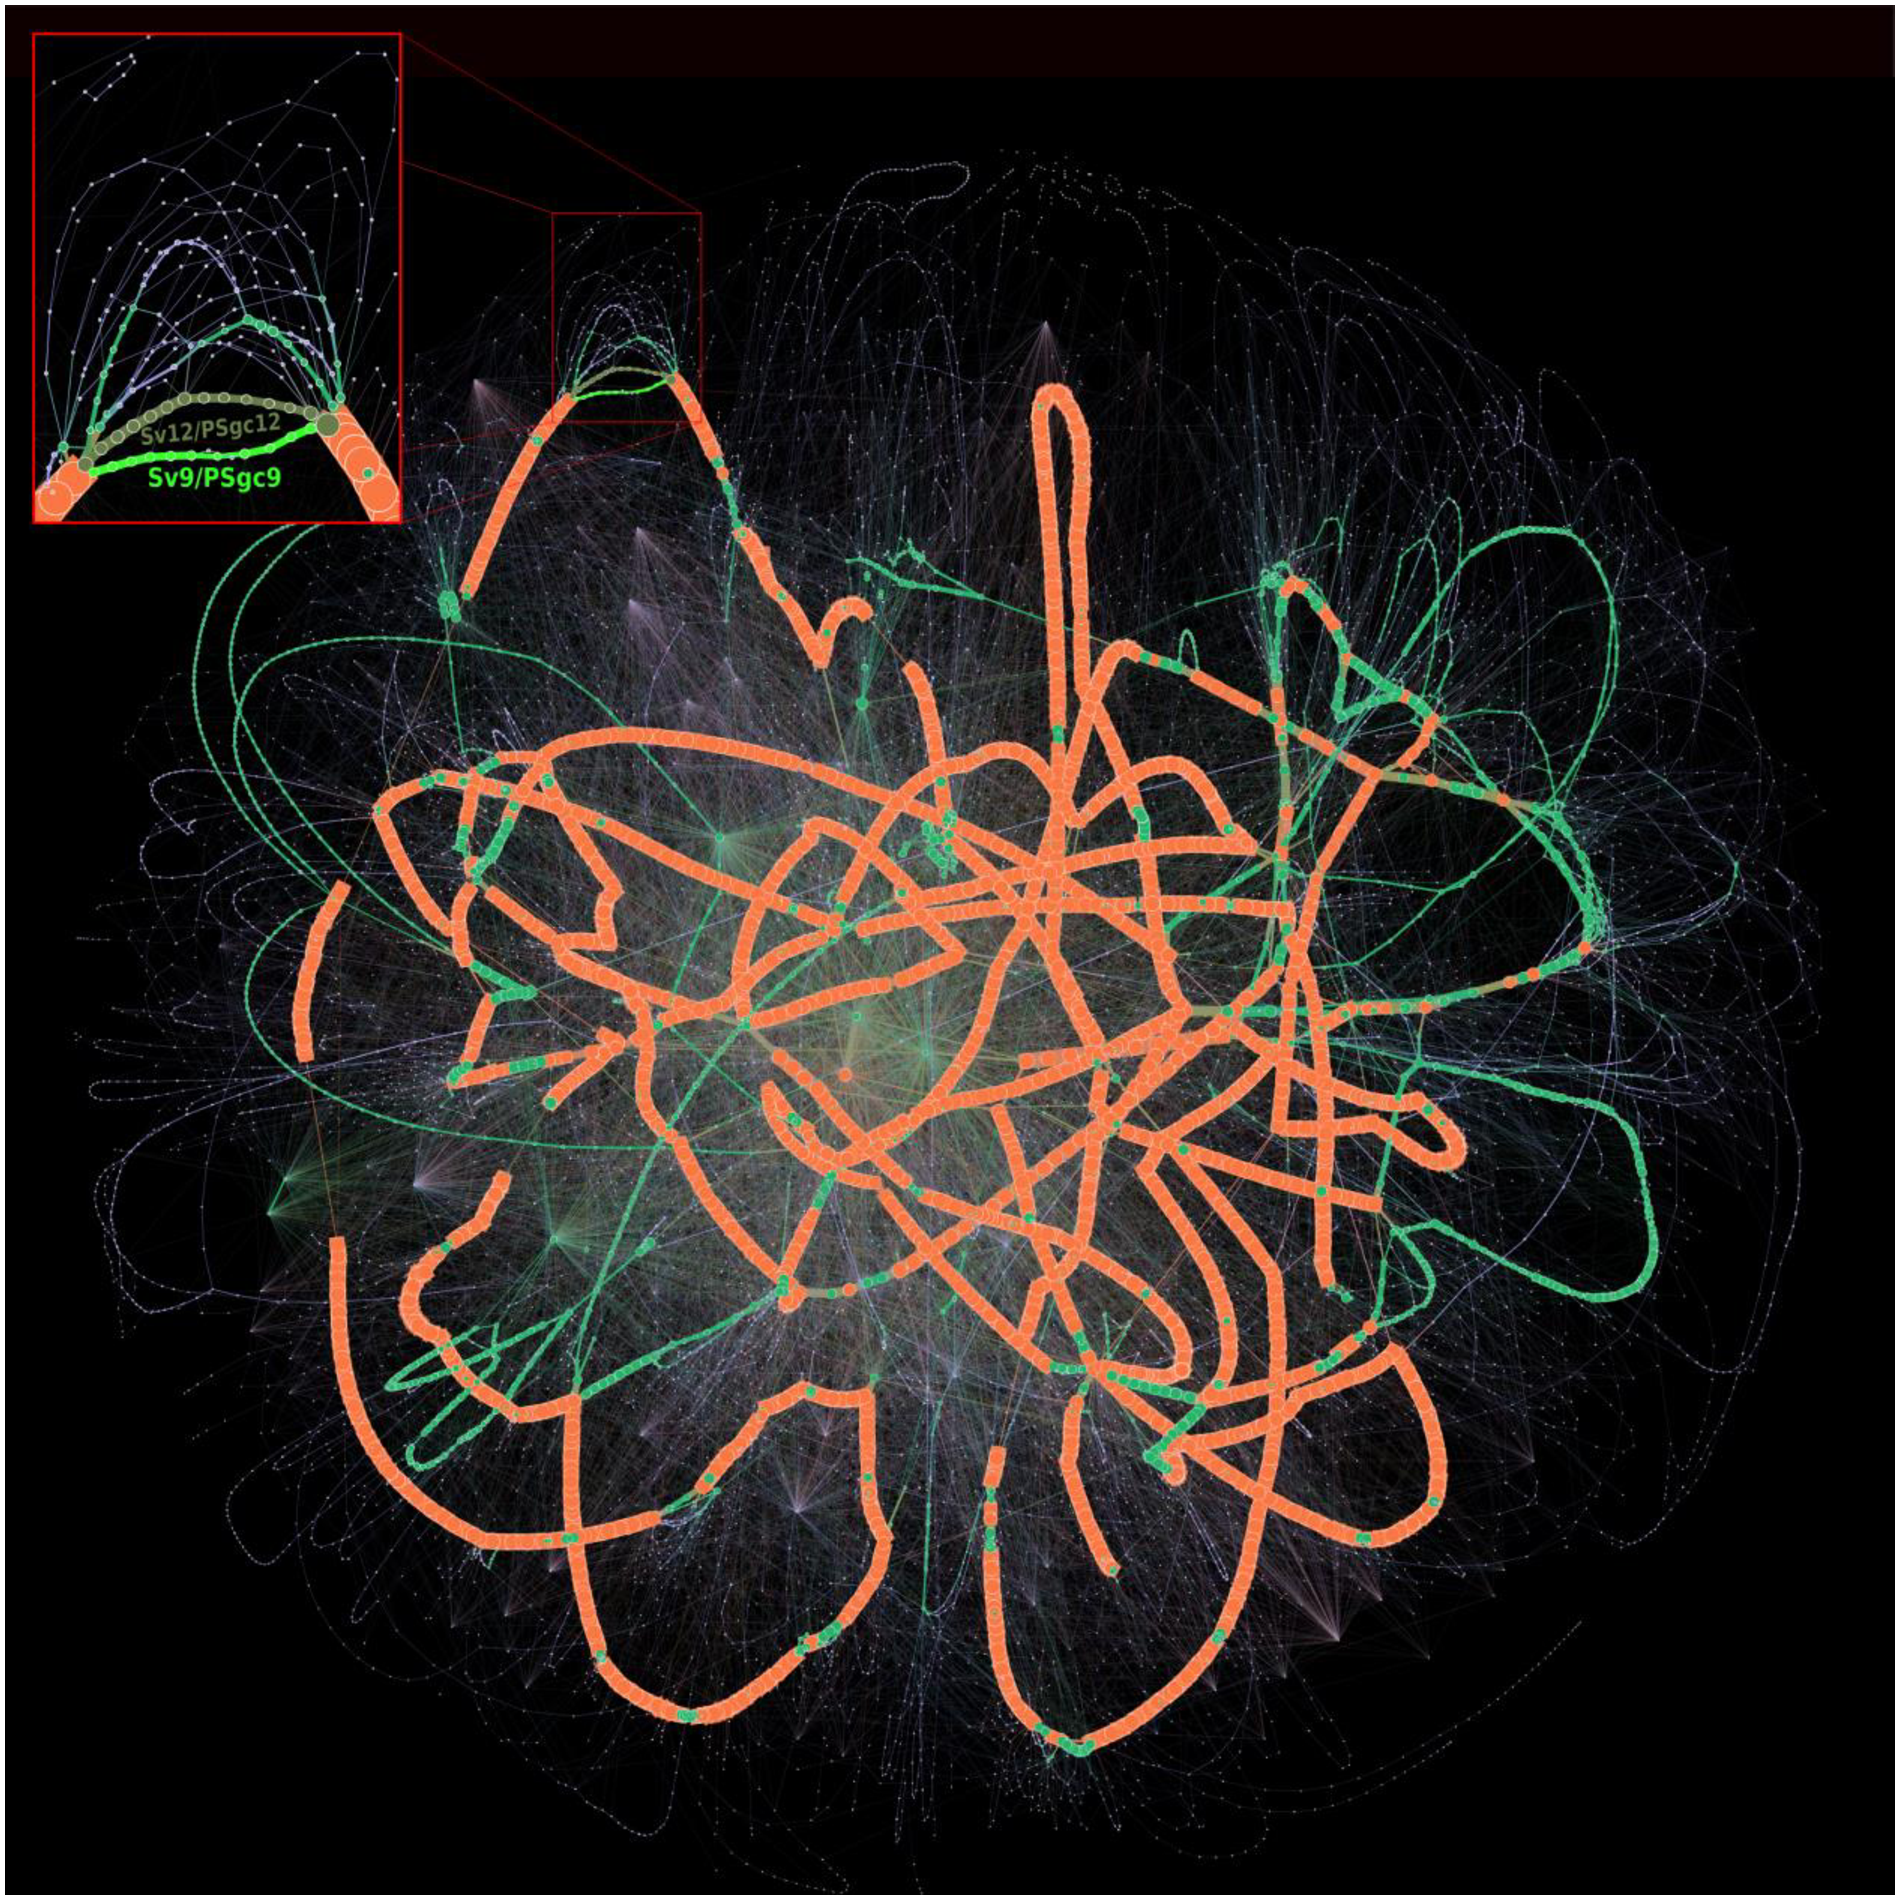
\includegraphics[width=0.6\linewidth]{images/pangenomeAcioneto.png}
    \caption[Graphe de pangénome de \textit{Acinetobacter baumannii}]{\textbf{Graphe de pangénome de \textit{Acinetobacter baumannii}.} Le pangénome est construit avec PPanGGOLiN à partir de 3117 génomes de \textit{A. baumannii}. Les arêtes reliant les familles \textit{persistent}, \textit{shell} et \textit{cloud} sont respectivement colorées en orange, vert et bleu. Les connexions entre familles de gènes appartenant à différentes partitions sont représentées par des couleurs mélangées. Pour améliorer la lisibilité, les familles comptant moins de 20 gènes ne sont pas affichées, bien qu'elles représentent 84,68 \% des n\oe uds (principalement des familles à un seul gène). Un encadré dans le coin supérieur gauche zoome sur une région ramifiée où plusieurs chemins alternatifs \textit{shell} et \textit{cloud} sont présents dans l'espèce. Cette région est impliquée dans la biosynthèse du principal antigène polysaccharidique de \textit{A. baumannii}. Les deux chemins les plus fréquents (Sv12/PSgc12 et Sv9/PSgc9) sont mis en avant en kaki et vert fluorescent.}
    \label{fig:pangenomeBaumannii}
\end{figure}

\section{La méthode PanRGP}

Le logiciel PPanGGOLiN intègre une méthode pour l'identification des régions de plasticité génomique et la prédiction des spots d'insertion, la méthode panRGP \cite{bazin_panrgp_2020}. Cette méthode repose sur l'utilisation du graphe de pangénome partitionné pour ne pas avoir à comparer l'ensemble des génomes (ce qui est déjà fait dans la construction du pangénome) et donc d'être plus efficace que les outils de génomique classique.

\subsection{Identification des régions de plasticité génomique}

Les régions de plasticité génomique sont des objets génomiques : la méthode de prédiction décrite dans la \autoref{fig:panRGP} est appliquée à chaque génome du pangénome, sur lesquels on a projeté les partitions du pangénome.

Pour chaque gène du génome, on calcule un score $s_g$ de manière séquentielle le long des contigs qui est égal au score du gène précédent auquel on applique une pénalité ou une prime en fonction de la partition du gène. Si le gène est \textit{shell} ou \textit{cloud}, on applique une prime correspondant à la somme de 2 constantes, $v$ qui favorise le gène variable et $\epsilon$ pour égaliser les résultats quelque soit le sens de lecture du contig. Si le gène est \textit{persistent}, on applique une pénalité $p$. Pour pénaliser la succession de gènes \textit{persistent}, la pénalité est exponentiellement proportionnelle au nombre ($n$) de gènes \textit{persistent} successifs précédents ($p^n$).   

Si le génome est linéaire, le premier gène de chaque contig aura un score de 0. Dans le cas des séquences circulaires, un premier gène est choisi et un score initial de 0 lui est attribué, puis l’algorithme assigne un score à tous les autres gènes. À la fin du contig, le gène avec un score de 0 est réévalué. Ce nouveau score sert de base pour exécuter une nouvelle boucle de calcul de score qui s'arrête dès qu'un gène obtient un score de 0 ou jusqu’à atteindre le dernier gène du contig.

\begin{figure}[htbp]
    \centering
    \includegraphics[width=0.8\linewidth]{images/panRGP.jpeg}
    \caption[PanRGP : vue d’ensemble de la méthode de détection des RGP]{\textbf{PanRGP : vue d’ensemble de la méthode de détection des RGP.} Les boîtes représentent les gènes codant des protéines : les couleurs orange, vert et bleu correspondent respectivement aux partitions \textit{persistent}, \textit{shell} et \textit{cloud}. Les boîtes en pointillés signalent les gènes appartenant à des familles multigéniques. Dans cet exemple, deux RGP sont détectées : RGP1 avec un score de 5 et RGP2 avec un score de 4. La valeur n associée à chaque gène correspond au nombre de gènes persistants consécutifs en aval. Les valeurs $f(g)$ représentent le résultat d'une fonction utilisée pour calculer le score de chaque gène ($s_g$). Ici, les paramètres par défaut p et v sont fixés respectivement à 3 et 1.}
    \label{fig:panRGP}
\end{figure}

Pour détecter les RGPs, l’algorithme parcourt chaque contig à la recherche du gène ayant le score le plus élevé, à condition qu’il dépasse le seuil $s_{min}$ (fixé par défaut à 4). Ce gène marque la fin initiale de la RGP. Ensuite, les gènes situés en amont sont ajoutés progressivement jusqu’à rencontrer un gène dont le score est nul. La région est alors considérée comme une RGP uniquement si elle contient un nombre de nucléotide supérieur au seuil minimal attendu $l_{min}$ (fixé par défaut à 3 000 bp). Enfin, le score de la RGP est recalculé en repartant du dernier gène détecté, en appliquant la même méthode de calcul que précédemment.

\subsection{Prédiction des spots d'insertion}

Les spots correspondent à des régions où de nombreux éléments se sont insérés au cours de l'évolution, et donc ce sont des régions fortement variables. Aux extrémités de chaque RGP, on sélectionne un nombre \textit{c} de gènes persistants non multigéniques, convertis en familles de gènes pour rendre l’algorithme indépendant de l’orientation.

\newpage

Un graphe $G(V, E)$ est construit, où chaque n\oe ud représente les bordures d’une RGP et chaque arête relie deux n\oe uds ayant des ensembles de familles de gènes similaires. Deux bords sont considérés comme proches si leurs \textit{e} premières familles sont identiques ou si leurs ensembles ordonnés se chevauchent d’au moins \textit{o} familles. Lorsque tous les bords de deux RGPs correspondent, une arête est ajoutée, et les composantes connexes du graphe définissent les spots, auxquels sont associées les RGPs correspondantes.

Les paramètres par défaut sont $c=3$, $e=1$, $o=2$. Chaque spot est évalué selon plusieurs métriques, comme le nombre de RGPs et de familles de gènes. Les RGPs sans $c$ gènes persistants consécutifs ne sont pas prises en compte, car elles sont soit incomplètes (bords de contigs), soit correspondent à des plasmides.

\section{La méthode PanModule}

Dans les génomes, et notamment dans les GIs et les spots, des groupes de gènes sont supposés avoir suivi la même histoire évolutive. Ces ensembles de gènes, cooccurrents et colocalisés, sont appelés des \textbf{modules conservés}. La méthode panModule \cite{bazin_panmodule_2021}, intégrée à PPanGGOLiN, permet de détecter ces modules depuis le graphe de pangénome partitionné. 

\newpage

Tout d'abord, un pangénome est reconstruit à partir des génomes, mais celui-ci intègre, en plus des arêtes de voisinage directes, des arêtes entre les familles séparées dans les génomes d'un espace intergénique inférieur à $t$ gènes. Lorsque $t > 1$, cela équivaut à appliquer une \textbf{fermeture transitive} partielle sur les graphes de génomes, ce qui permet de relier des familles même si leurs gènes ne sont pas directement adjacents. Cette approche est particulièrement utile lorsqu’un module génomique est interrompu par l’insertion d’un gène (comme une séquence d’insertion) ou lorsque des gènes ont été perdus à la suite d’un événement de délétion ou de pseudogénisation.

Les arêtes vont ensuite être filtrées selon deux \textbf{coefficients de similarité de Jaccard} :

\begin{equation}
J(v_i, e_{i,j}) = \frac{w_{e_{i,j}}}{w_{v_i}}, \quad J(v_j, e_{i,j}) = \frac{w_{e_{i,j}}}{w_{v_j}}
\label{eq:jaccard}
\end{equation}

où :
\begin{itemize}
    \item $w_{v_i}$ et $w_{v_j}$ correspondent au nombre de gènes associés aux familles $v_i$ et $v_j$, respectivement.
    \item $w_{e_{i,j}}$ représente le nombre de paires de gènes ayant servi à créer l’arête $e_{i,j}$ entre les nœuds $v_i$ et $v_j$.
\end{itemize}

Un seuil $s$ est défini comme la similarité minimale de Jaccard nécessaire pour considérer une arête comme appartenant à un module. Si les deux coefficients de Jaccard vérifient :

\begin{equation}
J(v_i, e_{i,j}) > s \quad \text{et} \quad J(v_j, e_{i,j}) > s
\end{equation}

alors l’arête est conservée ; sinon, elle est supprimée du graphe. De plus, les n\oe uds correspondant à des familles de gènes présentes dans moins de $m$ génomes sont également retirés.

Après cette phase de filtrage, les \textbf{composantes connexes} du graphe sont extraites à l’aide d’un algorithme de \textbf{parcours en largeur (BFS)} modifié. Une composante est considérée comme un \textbf{module prédit} si elle contient au moins trois n\oe uds appartenant aux familles \textit{shell}, \textit{cloud} ou multigéniques persistantes, selon la classification PPanGGOLiN. En revanche, les modules constitués de \textbf{familles persistantes non multigéniques} ne sont pas pris en compte. Ces familles correspondent généralement à des régions synténiques conservées dans la majorité des génomes étudiés, avec peu ou pas d’événements de réarrangement.

Les modules prédits peuvent ensuite être associés aux autres analyses de PPanGGOLiN, en identifiant sur quelles RGPs et dans quels spots sont retrouvés les modules.

\chapter{Évolution de PPanGGOLiN : présentation de la version 2}

PPanGGOLiN est un outil dont le développement a commencé (sur GitHub) en 2018. Avec plus de 2000 commits\footnote{ajout, suppression ou modification de code validé et marqué dans le système de gestion de version (ici Git)} actuellement, et 7 ans de développement, le code a connu de nombreuses évolutions. De plus, ces modifications sont l'\oe uvre de plusieurs développeurs qui se sont succédés et qui ont collaboré activement au projet.

Le développement de nouvelles méthodes, l'ajout de nouveaux outils, ou encore simplement le débogage devenaient de plus en plus lourds. De plus, dans le cadre de ma thèse, PPanGGOLiN allait être utilisé comme outil et certaines fonctionnalités devaient être améliorées. C'est avec cet objectif en tête que Jean Mainguy (ingénieur au LABGeM), Guillaume Gautreau (chercheur INRAE), Adelme Bazin (ingénieur de recherche), Alexandra Calteau (chercheuse CEA), David Vallenet (directeur de recherche CEA) et moi-même avons développé et proposé en janvier 2024 une version 2 de PPanGGOLiN. Cette nouvelle version contient de nouvelles fonctionnalités pour l'analyse des pangénomes, mais aussi de nombreuses améliorations techniques.

Dans ce chapitre, nous reviendrons sur les changements majeurs apportés dans la version 2 de PPanGGOLiN. D'autres changements plus anecdotiques ne seront pas abordés. Néanmoins, une des améliorations concerne l'écriture des notes de versions qui sont plus détaillées. Toutes les modifications sont alors visibles dans ces notes sur le GitHub de PPanGGOLiN \url{https://github.com/labgem/PPanGGOLiN/releases}.

\section{Nouvelles fonctionnalités et amélioration méthodologique}
\subsection{Developpement de nouvelles méthodes d’analyse}
\subsubsection{Recherche de contexte génomique}

\paragraph{Définition}

Le contexte génomique (\textit{Genomic Context}, GC) désigne l’organisation spécifique des gènes au sein d’un génome. Durant l'évolution, cette organisation va subir des pressions de sélection. Si elle se maintient conservée, on peut postuler que les gènes du GC sont impliqués dans un même processus biologique. C'est pourquoi, la recherche de GCs conservés dans les génomes est utilisée pour prédire la fonction de gènes inconnus en les associant à d'autres dont la fonction est connue. C'est le principe du coupable par association \cite{aravind_guilt_2000}. Rechercher un GC (ou un sous-ensemble de ce dernier) dans les génomes permet ainsi d'identifier des processus biologiques et des dérivés dans les génomes, comme le fait antiSMASH \cite{medema_antismash_2011}, en détectant spécifiquement les clusters de gènes biosynthétiques (BGCs).

\newpage

Une des méthodes de recherche de GC dans les génomes repose sur le voisinage des gènes dans les séquences. On considère des gènes comme fonctionnellement liés s’ils sont régulièrement retrouvés à proximité les uns des autres dans divers génomes, même sans être directement adjacents. Ce type de signal permet de détecter des associations fonctionnelles conservées, même entre des gènes non homologues. 

Cette approche est particulièrement intéressante dans le cadre des graphes de pangénome, comme ceux produits par PPanGGOLiN. Le graphe de pangénome intègre déjà l’information sur le voisinage direct des gènes à travers l’ensemble des génomes étudiés. Cela permet d’extraire efficacement le contexte génomique directement depuis le graphe. De plus, cette approche permet de capturer toute la diversité génomique d’un ensemble d’organismes : non seulement les gènes conservés dans toutes les souches, mais aussi les gènes accessoires, présents uniquement dans certaines d’entre elles. Ainsi, l’extraction du contexte génomique à partir d’un pangénome permet de mieux refléter la diversité biologique réelle tout en accélérant la prédiction fonctionnelle des gènes.

\paragraph{Méthode de recherche de contexte génomique}

L'algorithme de prédiction (\autoref{fig:searchCC}) s’inspire de celui proposé dans panModule \cite{bazin_panmodule_2021}. Cependant, contrairement à ce dernier, qui vise à extraire l’ensemble des contextes génomiques conservés, notre approche se focalise sur l’identification précise des contextes associés à un ensemble de protéines cibles. L’objectif est d’extraire, au sein du pangénome, les familles de gènes conservées dans le contexte de ces protéines.

La première étape consiste à aligner les gènes cibles (\textit{target}) avec les familles de gènes du pangénome. Cet alignement est effectué à l’aide de MMSeqs2 \cite{steinegger_mmseqs2_2017}, avec un seuil de 80 \% d'identité et 80 \% de couverture entre les séquences protéiques des gènes et celles des familles. Les familles correspondant aux séquences alignées sont alors étiquetées comme \textit{target} (représentées en bleu et orange dans la \autoref{fig:searchCC}).

\begin{figure}[htbp]
    \centering
    \includegraphics[width=\linewidth]{images/searchCC.png}
    \caption[Méthode de recherche du contexte génomique dans un graphe de pangénome]{\textbf{Méthode de recherche du contexte génomique dans un graphe de pangénome.}}
    \label{fig:searchCC}
\end{figure}

\newpage
À partir de ces familles \textit{target}, nous reconstruisons un sous-graphe du pangénome. Ce sous-graphe intègre non seulement les arêtes de voisinage direct, mais aussi des arêtes de transitivité reliant des familles situées à une distance $t$. Ainsi, l’algorithme capture non seulement les relations directes, mais aussi celles entre familles avoisinantes. Par exemple, dans la \autoref{fig:searchCC}, avec $t=1$, des arêtes de transitivité sont créées entre le gène bleu et les gènes vert et noir, ainsi qu'entre le gène violet et les gènes rouge et gris.

Pour limiter la taille du sous-graphe, un paramètre \textit{window} est introduit. Il contrôle le nombre de gènes adjacents — de part et d'autre de la \textit{target} — pris en compte pour la création des arêtes de transitivité.

Le sous-graphe obtenu forme alors une composante connexe intégrant l’ensemble des relations de voisinage jusqu’à la distance $t$. Un filtre de Jaccard (cf. \autoref{eq:jaccard}) est ensuite appliqué pour conserver uniquement les arêtes les plus pertinentes.

Enfin, nous extrayons toutes les composantes connexes contenant au moins une famille \textit{target}, représentant ainsi les contextes génomiques conservés autour des protéines cibles.

\subsubsection{Metadonnées}

Dans le cadre de l'ajout de nouvelles fonctionnalités à PPanGGOLiN, une première avancée que j'ai développée concerne l'ajout de \textbf{métadonnées} à l'ensemble des éléments du pangénome, incluant les gènes, contigs, génomes, familles, arêtes, RGPs, spots et modules. Le format attendu des métadonnées est particulièrement flexible, l'utilisateur fournit un fichier tabulé, ne nécessitant au minimum que l'identifiant de l'objet concerné dans le pangénome.  L’utilisateur peut ainsi associer des métadonnées de tout type, sans restriction de format. De plus, chaque métadonnée est liée à une source spécifique, ce qui permet à un même objet d’en contenir plusieurs, issues de différentes sources d’annotation. Pour assurer une gestion optimisée et performante, ces métadonnées sont directement enregistrées dans le fichier HDF5 du pangénome. Bien qu'elles ne soient pas directement exploitées pour l'analyse du pangénome, elles sont intégrées aux sorties générées par PPanGGOLiN afin de faciliter l'interprétation et l'exploration des résultats.

\subsubsection{Projection}

Pour faciliter l'exploration des résultats, une \textbf{nouvelle sortie de visualisation des données} a été développée en collaboration avec Jean Mainguy. Celle-ci permet de générer, pour chaque génome, un fichier JSON compatible avec Proksee \cite{grant_proksee_2023}. Grâce à cette fonctionnalité, il est désormais possible de visualiser un génome, sous forme circulaire (\autoref{fig:projection}), où les éléments du pangénome ont été intégrés, notamment les parties persistantes et variables, ainsi que les RGPs, spots et modules. Proksee permet également de lancer des analyses supplémentaires sur les génomes, comme CARD \cite{alcock_card_2023} pour annoter les gènes de résistance aux antibiotiques, CRISPRCasFinder \cite{couvin_crisprcasfinder_2018} pour la prédiction des systèmes CRISPR-Cas, ou encore Phigaro \cite{starikova_phigaro_2020} qui permet d'identifier les régions de prophages. 

\newpage
L'intégration de cette nouvelle sortie est d'autant plus intéressante dans une autre nouvelle fonctionnalité de PPanGGOLiN : la \textbf{projection} des résultats du pangénome sur un génome externe. En effet, il est désormais possible de comparer un nouveau génome au pangénome déjà calculé. Pour cela, les gènes du génome externe sont alignés aux séquences référentes des familles de gènes en utilisant MMSeqs2 \cite{steinegger_mmseqs2_2017}. Les gènes dont l'alignement dépasse un seuil défini d'identité et de couverture sont alors associés à une famille existante, tandis que les autres gènes forment chacun une nouvelle famille (singleton) attribuée à la partition du \textit{cloud}. Ainsi, l’ensemble des gènes du génome externe se voit assigner une partition, ce qui permet d’appliquer les algorithmes de prédiction des RGPs et d’associer les spots et les modules au génome étudié.

Enfin, cette fonctionnalité de projection prend également en compte les métadonnées, assurant ainsi la transmission des informations du pangénome aux gènes du génome externe. Cette intégration renforce la cohérence des analyses en permettant d’exploiter les annotations des utilisateurs pour une meilleure interprétation des résultats.

\begin{figure}[htbp]
    \centering
    \includegraphics[width=\linewidth]{images/projection.png}
    \caption[Principe de fonctionnement de la méthode de projection]{\textbf{Principe de fonctionnement de la méthode de projection.} Le génome sur lequel le pangénome est projeté, est un génome de la même espèce que ceux qui ont servi à construire le pangénome. Sur la droite, un exemple de sortie disponible dans PPanGGOLiN et généré dans les projections, le Proksee \cite{grant_proksee_2023} d'un génome de \textit{A. baumannii} où les résultats du pangénome ont été projeté.}
    \label{fig:projection}
\end{figure}

\subsubsection{Analyse comparée des RGPs}

Une nouvelle fonctionnalité a été intégrée à PPanGGOLiN pour permettre l’analyse comparative des RGPs entre plusieurs génomes d’un même pangénome. Désormais, il est possible de regrouper (clusteriser) les RGPs similaires  (\autoref{fig:rgpcluster_met}). Deux RGPs sont considérés comme partageant un contenu commun si leurs gènes appartiennent aux mêmes familles de gènes. À partir de cette définition, un score de correspondance du répertoire génique (\textit{Gene Repertoire Relatedness}, GRR) est calculé, soit sur la RGP la plus petite, soit sur la plus grande :

\begin{equation}
\begin{split}
GRR_{min} = \frac{\text{nombre de gènes partagés}}{\text{nombre de gènes de la plus petite RGP}} \\
GRR_{max} = \frac{\text{nombre de gènes partagés}}{\text{nombre de gènes de la plus grande RGP}}
\end{split}
\end{equation}

Le processus de clustering repose sur une modélisation par graphe. Chaque RGP est représentée sous forme d’un n\oe ud, et une arête est ajoutée entre deux n\oe uds si leur GRR dépasse un seuil défini (0,8 par défaut). Ainsi, chaque composante connexe du graphe correspond à un ensemble de RGPs partageant un même répertoire génique.

Les résultats du clustering sont disponibles soit sous forme d'un fichier tabulé récapitulant les regroupements obtenus, soit dans des outils de visualisation de graphe comme Gephi \cite{bastian_gephi_2009} ou Cytoscape \cite{shannon_cytoscape_2003}.

L’intégration des métadonnées prend de nouveau tout son sens. Il est possible d’annoter et de colorer les graphes en fonction des métadonnées associées aux gènes du pangénome, ce qui facilite l’interprétation biologique des clusters obtenus. Un exemple d’application est illustré en \autoref{fig:rgpcluster_app}, où le clustering des RGPs du pangénome de \textit{A. baumannii} a été réalisé. Les gènes ont été annotés avec CARD \cite{alcock_card_2023} pour identifier les éléments liés à la résistance aux antibiotiques. Deux clusters ont été extraits en guise d'exemple. Le cluster de gauche correspond à un ensemble de RGPs localisés dans un même spot (13). Parmi eux, trois RGPs sont associées à des \textbf{gènes de résistance aux antibiotiques }(n\oe uds en forme de triangle). Le cluster de droite regroupe des RGPs répartis sur huit spots distincts, révélant ainsi une mobilité plus variée dans les génomes. Contrairement au premier cluster, ces RGPs ne sont pas directement associées à des gènes de résistance. Cependant, d’autres métadonnées, par exemple des annotations métaboliques, pourraient être intégrées pour identifier des fonctions communes entre ces spots.

\begin{figure}[htbp]
    \centering
    \subfloat[Méthode de clusterisation des RGPs]{\includegraphics[width=\linewidth]{images/clusterRGPs.png}
    \label{fig:rgpcluster_met}}
    \hfill
    \subfloat[Application du clustering des RGPs sur le pangénome de \textit{A. baumannii} avec des métadonnées de résistance aux anitbiotiques (AMR)]{\includegraphics[width=\linewidth]{images/rgpclusterappli.png}
    \label{fig:rgpcluster_app}}
    \caption[Clustering des RGPs]{\textbf{Clustering des RGPs.}}
    \label{fig:rgpcluster}
\end{figure}

\subsection{Amélioration des procédures d'analyses}

\subsubsection{Lecture des fichiers d'annotation}

PPanGGOLiN permet la construction d'un graphe de pangénome à partir de séquences nucléiques et de génomes préalablement annotés. Les fichiers de génomes annotés (aux formats GFF ou GBFF) contiennent déjà les gènes ainsi que leurs coordonnées (contig, position, brin \dots). Ces fichiers peuvent également inclure des informations sur la fonction des gènes, des métadonnées relatives aux génomes et aux contigs, ainsi que la séquence des gènes ou des contigs eux-mêmes. Jusqu'à récemment, une partie de ces informations était ignorée par PPanGGOLiN. Désormais, elles sont lues et stockées dans le fichier de pangénome sous forme de métadonnées.

En nous intéressant à l'annotation fonctionnelle du pangénome, nous avons observé des divergences entre les séquences issues des fichiers d'annotation et celles correspondant aux gènes et aux familles de gènes. Nous avons notamment constaté que certaines coordonnées de gènes présentaient une complexité particulière et correspondaient à des événements biologiques spécifiques, tels que des décalages du cadre de lecture (\textit{frameshift}). Un ensemble de cas présentant des coordonnées atypiques a ainsi été identifié et est désormais correctement pris en charge dans PPanGGOLiN.

Ces améliorations ont conduit à une meilleure construction des familles de gènes, en corrigeant des séquences auparavant incorrectement tronquées ou décalées. Par ailleurs, elles ont permis d'améliorer la réécriture des séquences dans les fichiers de sortie, notamment ceux destinés à Proksee \cite{grant_proksee_2023}, et, par conséquent, la qualité des annotations fournies par les outils intégrés à cette plateforme.

\newpage

\subsubsection{Exécution de PPanGGOLiN via un fichier de configuration}

PPanGGOLiN intègre désormais la possibilité de générer un fichier de configuration. Ce fichier contient l’ensemble des commandes de PPanGGOLiN pouvant être exécutées ainsi que les paramètres spécifiques à chaque commande et les  globaux. A partir de ce fichier, PPanGGOLiN peut lancer une analyse \textit{de novo} sans préciser les paramètres de la ligne de commande. Ce fichier offre ainsi une alternative plus souple et organisée à l’exécution classique en ligne de commande. Il présente aussi plusieurs avantages.
(\textit{i}) Une exécution entièrement paramétrable des workflows. Jusqu’à présent, l’exécution de PPanGGOLiN dans un workflow reposait sur un nombre restreint de paramètres en ligne de commande. Cette limitation visait à éviter une surcharge des lignes de commande ainsi que d’éventuels conflits de nommage entre paramètres. Grâce aux fichiers de configuration, il devient possible de paramétrer entièrement un workflow, en définissant de manière explicite toutes les options requises. 
(\textit{ii}) Une intégration facilitée dans les pipelines d’analyse. L’utilisation de fichiers de configuration simplifie considérablement l’intégration de PPanGGOLiN dans des pipelines d’analyse. En effet, l’exécution d’outils en ligne de commande au sein de pipelines automatisés (souvent via des scripts Bash) peut poser plusieurs difficultés, telles que : une mauvaise interprétation des types de paramètres (par exemple, un entier lu comme une chaîne de caractères), des erreurs dans la gestion des chemins de fichiers, des conflits entre options spécifiques. L’emploi d’un fichier de configuration permet d’éliminer ces problèmes en standardisant et sécurisant la transmission des paramètres. Cette approche a notamment été adoptée lors de l’intégration de PPanGGOLiN dans MicroScope \cite{vallenet_microscope_2020}.

L’ajout des fichiers de configuration s’inscrit également dans les principes FAIR\footnote{Les principes FAIR visent à garantir que les données et les logiciels scientifiques soient faciles à retrouver (Findable), accessibles (Accessible), interopérables (Interoperable) et réutilisables (Reusable). Bien que ces principes aient été initialement conçus pour les données et le \textit{Big Data}, ils s’appliquent également aux outils bioinformatiques.}. En particulier, ils renforcent la reproductibilité des analyses. PPanGGOLiN permet ainsi de générer, à partir d’un pangénome, un fichier de configuration contenant toutes les options ayant permis sa construction. Cela garantit que, pour un même jeu de données, les analyses restent strictement reproductibles, favorisant ainsi une science plus ouverte et plus éthique. Cette avancée est particulièrement bénéfique dans un contexte de publication scientifique, où la transparence et la reproductibilité des analyses sont essentielles.

\newpage

\section{Optimisation technique}

Au-delà de l’ajout de nouvelles fonctionnalités, la version 2 de PPanGGOLiN a bénéficié de nombreuses améliorations visant à optimiser son efficacité, son ergonomie et sa maintenabilité. Parmi celles-ci, les optimisations techniques ont joué un rôle clé en réduisant la taille des fichiers générés, les temps de lecture ainsi que la mémoire utilisée.

\subsection{Amélioration de l'efficacité de PPanGGOLiN}

L’une des améliorations concerne l’optimisation du processus d’annotation des génomes. À cette fin, l’exécution de Prodigal \cite{hyatt_prodigal_2010} a été remplacée par l’intégration de Pyrodigal \cite{larralde_pyrodigal_2022}. Ce changement présente deux avantages principaux. 
Premièrement, la réduction des entrées/sorties (I/O) et l'amélioration de la gestion de la mémoire. Contrairement à l'exécution de Prodigal, qui nécessitait de générer des fichiers intermédiaires contenant les résultats d’annotation, Pyrodigal retourne directement les annotations sous forme d’objets Python utilisables par PPanGGOLiN. Cette approche permet de ne pas avoir à écrire et lire des fichiers intermédiaires pour chaque génome, réduisant ainsi l’empreinte mémoire et améliorant l’efficacité des opérations d’I/O. Deuxièmement, Pyrodigal intègre plusieurs améliorations au moteur de Prodigal, notamment une optimisation du calcul du score de connexion. Ce score est utilisé pour évaluer la probabilité d’une transition entre deux codons en fonction de divers critères (cadre de lecture, type de codon – initiation ou stop –, orientation du brin\dots). Comme l’a souligné Larralde \cite{larralde_pyrodigal_2022}, le calcul du score de connexion sur de longues séquences peut être coûteux en temps de calcul. Pyrodigal améliore ce processus en implémentant un filtrage heuristique, qui permet d’ignorer les connexions clairement invalides dès le départ. De plus, Pyrodigal exploite les fonctionnalités SIMD (Single Instruction, Multiple Data) des CPU modernes pour traiter plusieurs n\oe uds de calcul simultanément. Cela permet de traiter 8 n\oe uds avec les fonctionnalités NEON et SSE2, et 16 n\oe uds avec AVX2 (\autoref{fig:pyrodigal}). Ces optimisations réduisent le temps de calcul et améliorent significativement l’efficacité globale de la prédiction des gènes dans PPanGGOLiN.

\begin{figure}[htbp]
    \centering
    \includegraphics[width=0.8\linewidth]{images/pyrodigal.png}
    \caption[Évaluation des performances de calcul des scores de connexions]{\textbf{Évaluation des performances de calcul des scores de connexion.} L'évaluation est réalisé avec différents backends SIMD pour le filtre heuristique (SSE2 ou AVX2), avec un backend générique (\textit{Generic}) ou sans activer le filtre (\textit{None}). Chaque séquence a été traitée 10 fois sur un processeur \textit{i7-10710U} à 1,10 GHz. Extrait de \cite{larralde_pyrodigal_2022}}
    \label{fig:pyrodigal}
\end{figure}

Toujours dans l'objectif d'amélioration de l’efficacité de PPanGGOLiN, les fonctions de lecture ont été revues, afin de réduire le temps de chargement des données et l’utilisation de la mémoire. 
Pour atteindre cet objectif, plusieurs modifications ont été apportées à la manière dont les objets du pangénome sont interconnectés, afin de limiter le chargement de données inutiles. Dans PPanGGOLiN, la structure hiérarchique des objets implique, par exemple qu’un gène appartient à un contig, lequel est lui-même rattaché à un génome. Or, dans certaines commandes, le chargement des gènes entraînait systématiquement celui des contigs et des génomes, augmentant ainsi le temps d’exécution. Pour pallier ce problème, nous avons réorganisé ces dépendances et réécrit plusieurs fonctions de lecture afin de rendre l’accès aux données plus sélectif et plus efficace.

L’une des améliorations les plus significatives concerne la lecture des spots. Une réécriture de cette fonction a permis une réduction drastique du temps de lecture. Sur un pangénome de 3 083 génomes de \textit{E. coli}, le temps de lecture de 2 036 spots est passé de 25 minutes (dans un temps total de lecture du pangénome de 36 minutes) à seulement 3,5 secondes (pour un temps total réduit à 9 minutes et 38 secondes)\footnote{Cette amélioration est particulièrement visible sur les pangénomes de grande taille contenant un nombre important de spots, ce qui explique pourquoi le problème n’avait pas été détecté auparavant.}.

Dans cette même optique, des améliorations ont également été apportées à l’écriture des séquences (nucléotidiques et protéiques). Dans les versions précédentes de PPanGGOLiN, pour faciliter le filtrage des séquences demandées par l’utilisateur, l’ensemble du pangénome et de ses objets était chargé en mémoire, ce qui entraînait une consommation importante de ressources. Désormais, les séquences sont directement extraites du fichier HDF5, évitant ainsi la recréation systématique des objets du pangénome et réduisant significativement l’utilisation de la mémoire.

Avec l’augmentation continue du nombre de génomes disponibles, les pangénomes générés par PPanGGOLiN sont devenus de plus en plus volumineux. Malgré une structure de stockage compacte, reposant sur le package PyTable \cite{team_pytables_2002}, la taille des fichiers HDF5 a considérablement augmenté, en raison du nombre croissant de génomes et des nouvelles fonctionnalités enrichissant les données stockées.
Pour remédier à ce problème, l’architecture interne du fichier HDF5 a été revue afin d’éliminer les redondances, en particulier dans l’annotation des gènes et de leur séquence. En effet, entre différents génomes, les gènes peuvent partager des caractéristiques communes telles que leur position, leurs coordonnées ou encore leur orientation sur le brin. Or, ces informations étaient systématiquement dupliquées dans l’ancienne structure. Afin de réduire cette redondance, une table de référence a été mise en place pour centraliser ces informations et leur attribuer un identifiant unique, à la manière d’une base de données relationnelle. Chaque gène peut ainsi être associé à son annotation optimisée, sans nécessiter la répétition de ses caractéristiques dans l’ensemble du pangénome.
Cette optimisation a permis une réduction significative de la taille des fichiers HDF5. Comme illustré en \autoref{fig:ppanggoSize}, la taille des pangénomes a été divisée par 3,5 pour un ensemble de 1 000 génomes, et par 6,5 pour un pangénome de 2 500 génomes.
Au-delà du gain en espace de stockage, cette amélioration contribue également à l’accélération des temps de lecture. En effet, elle participe à la lecture non systématique des informations liées aux gènes lors du chargement du pangénome, ce qui allège le processus et améliore les performances globales de l’outil.

\begin{figure}
    \centering
    \includegraphics[width=.8\linewidth]{images/benchPPanGGO.png}
    \caption[Taille des fichiers de pangénome entre la version 1 et 2 de PPanGGOLiN]{\textbf{Comparaison des tailles des fichiers de pangénome entre la version 1 et 2 de PPanGGOLiN.}}
    \label{fig:ppanggoSize}
\end{figure}

Ces optimisations rendent PPanGGOLiN plus performant, plus rapide et plus adapté aux analyses pangénomiques de grande échelle, tout en maintenant une gestion efficace des ressources.

\subsection{Optimisation du code : lisibilité, maintenance, tests et processus de mise à jour}

En tant que logiciel open source, le code de PPanGGOLiN est accessible à tous, conformément aux principes de la science ouverte. Ce choix présente plusieurs avantages : il permet à la communauté d’utilisateurs de signaler d’éventuels comportements inattendus (problèmes de performance, bugs, \textit{etc}.), mais aussi de contribuer directement à l’amélioration du logiciel en proposant des corrections ou des optimisations.
Afin d’assurer la pérennité et la maintenabilité du projet, nous avons entrepris une révision complète du code, avec pour objectif principal de le rendre plus lisible, homogène et facile à maintenir pour les développeurs actuels et futurs.

\subsubsection{Mise en place de bonnes pratiques de développement}

La première étape du reformatage a consisté à aligner PPanGGOLiN avec les versions maintenues et corrigées de Python. Les packages les plus utilisés suivent également cette logique. En mettant à jour le code pour être compatible avec les versions récentes de Python, nous bénéficions des dernières mises à jour des packages, ainsi que des optimisations et corrections apportées par le langage lui-même. Ainsi, nous sommes passés de Python 3.8 à Python 3.12.

Pour améliorer la lisibilité et garantir une cohérence au sein du code, nous avons introduit un ensemble de règles et de processus applicables pour tous les développeurs. La première étape a été l’adoption des bonnes pratiques de codage en Python, en suivant les recommandations des PEP (\textit{Python Enhancement Proposals}).
L’application de ces directives présente plusieurs bénéfices. Premièrement, le code est plus structuré et lisible. Par exemple, les conventions de nommage permettent d’identifier rapidement la nature des variables et objets :

\begin{itemize}
    \item Nom des classes en CamelCase (\textit{e.g.} GeneCluster)
    \item Constantes en majuscules (\textit{e.g.} MAX\textunderscore ITERATIONS)
    \item Fonctions et méthodes en snake\textunderscore case (\textit{e.g.} compute\textunderscore similarity\textunderscore score)
\end{itemize}

Cette homogénéité facilite la lecture et la compréhension du code par tous les contributeurs. Deuxièmement, les règles PEP permettent de mettre en place des micro-optimisations pour de meilleures performances. Par exemple, en privilégiant l’utilisation de générateurs plutôt que des listes temporaires, ce qui permet d’optimiser l’utilisation de la mémoire.

Afin de faciliter l’application de ces règles et d’assurer leur respect de manière systématique, nous avons intégré le package python Black (\url{https://github.com/psf/black}) pour le formatage automatique du code. Lors de chaque mise à jour du code sur GitHub, Black est exécuté automatiquement pour reformater le code selon les standards des PEP. Cette automatisation garantit une cohérence stylistique, réduit la charge de travail des développeurs et simplifie la gestion des contributions extérieures.

Grâce à ces améliorations, le code de PPanGGOLiN devient plus clair, plus performant et plus facile à maintenir, assurant ainsi une plus grande longévité au projet et une meilleure collaboration au sein de la communauté open source.

\subsubsection{Maintenance et test du code}

PPanGGOLiN est avant tout un projet de recherche scientifique, ce qui implique des mises à jour fréquentes pour intégrer de nouvelles fonctionnalités et améliorer ses performances. Toutefois, ces modifications peuvent introduire des bogues susceptibles d’altérer la fiabilité des analyses. Afin de garantir la stabilité et la robustesse du logiciel, nous avons grandement amélioré la stratégie de tests automatisés, couvrant différents niveaux de validation.

\paragraph{Tests unitaires : validation des fonctionnalités élémentaires}

Les premiers tests mis en place sont des tests unitaires, qui permettent de vérifier le comportement individuel des fonctions. Ces tests s’assurent que chaque fonction produit bien le résultat attendu, et qu’elle génère les erreurs appropriées en cas d’entrée invalide. Actuellement, l'ensemble des classes sont testées et ainsi qu'une grande partie des fonctions.

\newpage

\paragraph{Tests d’intégration : validation des interactions entre fonctions}

Nous avons également mis en place des tests d'intégration, visant à évaluer le comportement global du logiciel lorsque plusieurs fonctions interagissent. En effet, une fonction peut répondre comme attendu de manière isolée tout en produisant des comportements imprévus lorsqu'elle est combinée à d'autres modules. Ces tests permettent donc de garantir la cohérence de l'ensemble du programme. Cependant, leur mise en \oe uvre reste complexe en raison des nombreuses interactions entre les fonctions dans PPanGGOLiN, ce qui limite la couverture de cette approche à une partie restreinte du code.

\paragraph{Tests fonctionnels : validation du comportement des commandes}

Enfin, nous avons introduit des tests fonctionnels, qui vérifient le comportement des commandes complètes. Pour cela, des fichiers de résultats de référence ont été préchargés, permettant de comparer automatiquement les nouvelles sorties avec les résultats attendus. Cette approche garantit que les évolutions du code n’altèrent pas l’exactitude des analyses produites par PPanGGOLiN. Toutes les commandes de PPanGGOLiN sont testées en prenant en compte tous les paramètres.


Lors d'une mise à jour du code, un workflow automatique est exécuté et permet de vérifier que le code est bien fonctionnel. Grâce à cette infrastructure de tests, le code est désormais plus robuste, limitant ainsi l’introduction de bogues imprévus et assurant la fiabilité des résultats scientifiques générés par le logiciel.

\subsubsection{Amélioration de l'expérience utilisateur}

PPanGGOLiN est un logiciel conçu pour les microbiologistes, dont l’expertise principale n’est pas nécessairement l’informatique. Il est donc essentiel de garantir une expérience utilisateur fluide, en facilitant aussi bien l’installation que l’utilisation du logiciel.

Un premier effort a été porté sur la réécriture complète de la documentation, afin de la rendre plus claire, plus structurée et mieux adaptée aux besoins des utilisateurs. Désormais, elle comprend :

\begin{itemize}
    \item Une section d’installation détaillant plusieurs méthodes adaptées à différents environnements,
    \item Un guide de prise en main rapide pour permettre aux utilisateurs d’exécuter rapidement PPanGGOLiN et ses principaux workflows,
    \item Des sections approfondies décrivant en détail chaque commande et analyse réalisable,
    \item Un guide dédié aux développeurs, recensant les bonnes pratiques et les processus de développement spécifiques à PPanGGOLiN.
\end{itemize}

De plus, la documentation est maintenant disponible sur ReadTheDocs, ce qui la rend plus accessible, mieux référencée et conforme aux principes FAIR.

\newpage

Un autre aspect clé de l’amélioration de l’expérience utilisateur concerne la gestion des erreurs. Afin de rendre les messages d’erreur plus explicites et plus informatifs, nous avons entrepris une révision complète de leur génération.
Les erreurs liées à une mauvaise utilisation par l’utilisateur sont maintenant décrites de manière plus claire et pédagogique. Les erreurs techniques, destinées aux développeurs, sont quant à elles plus précises, facilitant ainsi l’identification rapide de l’origine du problème. De plus, un plus large éventail de messages a été introduit pour couvrir davantage de cas d’erreur et améliorer la gestion des exceptions.


Grâce à ces améliorations, PPanGGOLiN devient plus intuitif pour les microbiologistes et plus facile à maintenir pour les développeurs, garantissant ainsi une expérience utilisateur optimisée.




\chapter{Application à l'étude de la dégradation du D-Apiose}

Le D-Apiose est un sucre de type pentose, principalement retrouvé dans la paroi cellulaire des plantes vasculaires, mais également présent en tant que métabolite secondaire \cite{picmanova_apiose_2016}. Chez les bactéries, plusieurs voies de dégradation du D-Apiose ont été identifiées \cite{carter_functional_2018}. Parmi celles-ci, la voie de la transcétolase non oxydante (\autoref{fig:apiosePathway}) constitue un mécanisme clé. Cette voie permet la conversion du D-Apiose en D-xylulose 5-phosphate, un métabolite intermédiaire central impliqué dans de nombreuses voies métaboliques essentielles. La voie de la transcétolase non oxydante a été détectée chez diverses bactéries du sol, notamment \textit{Actinobacillus succinogenes} et \textit{Bacteroides vulgatus}, ainsi que chez plusieurs espèces du genre \textit{Pectobacterium}.

En collaboration avec Guilhem Royer (AP-HP) et Erick Denamur (IAME), le LABGeM a identifié une voie alternative chez \textit{Escherichia coli}, où l'isomérase de la première réaction est remplacée par une succession de deux oxydoréductases. Cette voie a été initialement identifiée spécifiquement dans les \textit{Sequence Types} (ST) 131 et 14 de \textit{E. coli}, des souches pathogènes connues pour leur multirésistance aux antibiotiques et leur implication dans les bactériémies\footnote{Infection bactérienne présente dans le sang.} \cite{schembri_molecular_2015,de_korne-elenbaas_putative_2023}. Ces souches colonisent principalement le tube digestif, où la capacité à dégrader le D-Apiose pourrait conférer un avantage sélectif, améliorant ainsi le \textit{fitness} de ces pathogènes.

Dans ce cadre, j’ai contribué au projet en explorant les pangénomes afin d’identifier le contexte génomique associé à la fois à la voie classique (transcétolase non oxydante) et à la voie alternative de dégradation du D-Apiose.

\begin{figure}[htbp]
    \centering
    \includegraphics[width=0.75\linewidth]{images/ApiosePathway.png}
    \caption[Voie de dégradation du D-Apiose par la transcétolase non oxydante]{\textbf{Voie de dégradation du D-Apiose par la transcétolase non oxydante.} (a) Métabolites et réactions de la voie. La première réaction (en vert) correspond à l'isomérisation du D-Apiose en D-Apulose, catalysée par la D-Apiose isomérase. Le D-Apulose est ensuite phosphorylé en D-Apulose 4-phosphate (en rouge) par l’action d’une kinase. Enfin, la dernière transformation (en bleu) est catalysée par la transcétolase, qui permet la production du D-xylulose 5-phosphate. (b) Contexte génomique de la voie de dégradation chez cinq espèces bactériennes. Les gènes impliqués sont représentés par des flèches colorées, dont la couleur correspond à l’enzyme codée. Les gènes gris codent des SBP (protéines de liaison spécifiques) impliqués dans la reconnaissance du D-Apiose, tandis que les gènes noirs codent des composants d’un système de transport ABC. Extrait de \cite{carter_functional_2018}.}
    \label{fig:apiosePathway}
\end{figure}

\section{Recherche du contexte génomique chez les procaryotes}

Nous avons commencé par rechercher la voie de dégradation du D-Apiose, à la fois sous sa forme classique (transcétolase non oxydante) et sous sa forme alternative, dans les espèces procaryotes. Pour cela, nous avons analysé le contexte génomique associé aux six protéines clés impliquées dans ces voies. Ces protéines incluent : 3 enzymes communes aux deux voies, les deux sous-unités de la transcétolase et la kinase; une enzyme spécifique à la voie classique l'isomérase; 2 enzymes spécifiques à la voie alternative, les oxydoréductases.

L’analyse du contexte génomique a été réalisée sur un ensemble de 1 429 pangénomes d’espèces, générés à l’aide de l’outil PPanGGOLiN\footnote{Les pangénomes ont été élaborés dans le cadre du projet PanGBank, visant à constituer une base de données de pangénomes d’espèces.}. Ces pangénomes ont été construits à partir de 152 717 génomes issus de la base de données RefSeq \cite{pruitt_ncbi_2007}, en utilisant la taxonomie GTDB \cite{parks_standardized_2018} pour organiser les génomes par espèce (version RefSeq/GTDB : 220).

\newpage

Le GC de dégradation du D-Apiose a été identifié dans 125 espèces, réparties sur 43 genres, 17 familles, 15 ordres, 7 classes et 4 phylums (\autoref{fig:PhyloTreeApiose}). Parmi ces familles, les \textbf{Enterobacteriaceae} sont les plus représentées (66 espèces), suivies des \textbf{Rhizobiaceae} (23 espèces) et des \textbf{Pseudomonadaceae} (12 espèces). Cette répartition suggère que la voie de dégradation du D-Apiose est relativement fréquente chez les bactéries.
L’analyse de la distribution des données au sein des partitions du pangénome révèle que cette voie est principalement associée à un contexte \textit{persistent}, avec 28 genres sur 43 présentant une majorité de familles classées dans cette même partition.

Parmi les contextes identifiés, seules 7 espèces présentent la voie classique de dégradation du D-Apiose. Six d’entre elles appartiennent au genre \textit{Pectobacterium} : \textit{P. atrosepticum}, \textit{P. brasiliense}, \textit{P. parmentieri}, \textit{P. carotovorum}, \textit{P. versatile} et \textit{P. polare}. La septième espèce, \textit{Novosphingobium capsulatum}, appartient à la famille des \textit{Sphingomonadaceae} et est représentée en bleu-vert clair sur la \autoref{fig:PhyloTreeApiose}. Contrairement aux espèces du genre \textit{Pectobacterium}, où le contexte génomique est retrouvé dans la partition \textit{persistent}, celui de \textit{N. capsulatum} se situe dans la partition \textit{shell}, ce qui pourrait suggérer un transfert horizontal de gènes (HGT) entre ces espèces.

Par ailleurs, 3 espèces possèdent une version hybride entre la voie classique et la voie alternative, caractérisée par la présence simultanée de l’isomérase et des 2 oxydoréductases. Deux d’entre elles appartiennent à la famille des \textit{Sphingomonadaceae}, à savoir \textit{Sphingobium yanoikuyae} et \textit{Sphingomonas koreensis}, tandis que la troisième, \textit{Klebsiella aerogenes}, appartient aux \textit{Enterobacteriaceae}. La présence de voies hybrides dans certaines espèces pourrait refléter une adaptation évolutive conférant une plus grande flexibilité métabolique en fonction des conditions environnementales.

\newpage

Enfin, des contextes partiels ont été détectés dans 13 espèces. Dix d’entre elles appartiennent à la famille des \textit{Enterobacteriaceae}, incluant \textit{Salmonella diarizonae}, \textit{Atlantibacter hermannii}, \textit{Yersinia enterocolitica}, \textit{Leclercia adecarboxylata}, \textit{Citrobacter youngae}, \textit{Yersinia bercovieri}, \textit{Kosakonia radicincitans}, \textit{Yersinia mollaretii}, \textit{Yersinia massiliensis} et \textit{Yersinia intermedia}. Deux autres espèces, \textit{Paracidovorax avenae} et \textit{Paracidovorax citrulli}, appartiennent à la famille des \textit{Burkholderiaceae}, tandis que \textit{Clostridioides difficile} représente la famille des \textit{Peptostreptococcaceae}. L’existence de ces contextes partiels pourrait être attribuée à la présence d’autres voies métaboliques alternatives, comme proposé par Carter \textit{et al.} \cite{carter_functional_2018}, ou être liée à la spécificité de l’isomérase au genre \textit{Pectobacterium}. L’analyse de la base de données UniProt \cite{the_uniprot_consortium_uniprot_2025} suggère en effet que cette enzyme présente une faible similarité avec celles d’autres organismes, ce qui pourrait expliquer l’absence apparente de la voie classique dans certaines espèces, alors qu’un homologue fonctionnel pourrait exister.

Des recherches complémentaires seront nécessaires pour mieux comprendre les implications fonctionnelles de ces variations et explorer les mécanismes évolutifs sous-jacents.

\begin{figure}[htbp] 
    \centering
    \includegraphics[width=\textwidth]{images/phylogenetic_tree_with_pies.png}
    \caption[Arbre taxonomique des procaryotes étiqueté par la présence de la voie de dégradation du D-Apiose]{\textbf{Arbre taxonomique des procaryotes étiqueté par la présence de la voie de dégradation du D-Apiose.} Si une branche existe alors un GC a été détecté sinon l'embranchement n'est pas créé. Les feuilles de l'arbre représente le niveau taxonomique du genre. Les \textit{pie chart} en bout de branche, représente la proportion de GC trouvé dans chaque partition du pangénome, indépendamment de la forme de la voie (classique, alternative, hybride ou partielle).} 
    \label{fig:PhyloTreeApiose}
\end{figure}

Nous avons ensuite centré notre étude sur la famille des Enterobacteriaceae, où la voie de dégradation du D-Apiose avait été initialement identifiée \cite{carter_functional_2018} et à laquelle \textit{Escherichia coli} appartient.
Comme l'illustre la \autoref{fig:clustermap_entero}, le contexte génomique est principalement retrouvé dans la partition \textit{persistent} (16 espèces), suivie de la partition \textit{shell} (8 espèces) et enfin de la partition \textit{cloud} (5 espèces). 
Ces espèces appartiennent à plusieurs genres bactériens, notamment Klebsiella, Citrobacter, Serratia et Escherichia. La majorité d’entre elles sont connues pour être des pathogènes humains, partageant un habitat commun : le tube digestif. D’un point de vue phylogénétique et taxonomique, ces bactéries sont étroitement apparentées à des espèces vivant dans les sols, où la dégradation du D-Apiose issu des plantes constitue un avantage sélectif. C’est notamment le cas de \textit{Pantoea vagans}, une espèce isolée à partir de feuilles d’eucalyptus \cite{brady_pantoea_2009}.
La présence de la voie alternative dans la partie variable du pangénome suggère une acquisition par transfert horizontal, au cours de laquelle cette nouvelle voie métabolique aurait été transférée des bactéries vivant dans les écosystèmes du sol vers celles colonisant le microbiote intestinal et gastrique.

\begin{figure}[htbp] 
    \centering
    \includegraphics[width=.9\textwidth]{images/clustermap.png}
    \caption[Prédiction du contexte de dégradation du D-apiose dans les pangénomes des Enterobacteriaceae]{\textbf{Prédiction du contexte de dégradation du D-apiose dans les pangénomes des Enterobacteriaceae.}} 
    \label{fig:clustermap_entero}
\end{figure}

\newpage

\section{Analyse du pangénome de \textit{Escherichia coli}}

Nous avons ensuite recentré notre analyse sur l’espèce \textit{Escherichia coli}, dans laquelle la voie de dégradation du D-Apiose impliquant deux oxydoréductases avait été identifiée. Pour cela, nous avons exploité le pangénome construit précédemment à partir des bases de données RefSeq et GTDB \cite{pruitt_ncbi_2007,parks_standardized_2018}, dont la composition est indiquée dans le \autoref{tab:E_coli_pangenome}.

Le pangénome de \textit{E. coli} (\autoref{fig:pangenomeColi}) est majoritairement composé de familles variables (points bleus), avec des chemins \textit{persistent} (en orange) correspondant aux régions conservées. Au sein de ces chemins, on retrouve des régions variables, constituées d’éléments \textit{shell} (verts) et \textit{cloud}. Ces zones correspondent généralement à des spots d’insertion, où sont localisées des régions génomiques plastiques (RGPs). C’est dans ces régions variables que nous avons recherché le contexte génomique de la voie de dégradation du D-Apiose.


\begin{table}[htbp]
    \centering
    \begin{tabular}{|l|l|l|}
    \hline
    \textbf{Génomes} & \textbf{Gènes} & \textbf{Familles} \\
    \hline
    2006 & 9334727 & 57444 \\
    \hline
    \hline
    \textit{\textbf{Persistent}} & \textit{\textbf{Shell}} & \textit{\textbf{Cloud}} \\
    \hline
    3167 & 7960 & 46317\\
    \hline
    \hline
    \textbf{RGPs} & \textbf{Spots} & \textbf{Modules} \\
    \hline
    164573 & 1968 & 2089 \\
    \hline
    \end{tabular}
    \caption[Composition du pangénome de \textit{E. coli}]{\textbf{Composition du pangénome de \textit{E. coli}.} Le pangénome a été généré avec PPanGGOLiN et utilise les génomes de RefSeq \cite{pruitt_ncbi_2007} en suivant la taxonomie de GTDB \cite{parks_standardized_2018}}
    \label{tab:E_coli_pangenome}
\end{table}

\begin{figure}[htbp] 
    \centering
    \includegraphics[width=.9\textwidth]{images/pangenome_ecoli.png}
    \caption[Graphe de pangénome de \textit{E. coli}]{\textbf{Graphe de pangénome de \textit{E. coli}.} Le graphe est visualisé avec Gephi \cite{bastian_gephi_2009}. L'algorithme de spatialisation utilisé est \textit{Force Atlas 2} avec une gravité forte et une échelle à 5 000.} 
    \label{fig:pangenomeColi}
\end{figure}


L’analyse a révélé que le contexte génomique associé à cette voie est localisé dans le spot 181 du pangénome (\autoref{fig:spot_apiose}). Ce spot d’insertion est identifié dans 62 génomes, chacun contenant une seule RGP. Parmi ces génomes, 31 possèdent le contexte de dégradation du D-Apiose. Comme illustré dans la \autoref{fig:spot_apiose}, ce contexte est également associé au module 752, qui est spécifique de la voie métabolique.

L’analyse de la composition en familles du module met également en évidence la conservation de plusieurs familles de gènes qui, bien que ne jouant pas un rôle enzymatique direct, sont essentielles au fonctionnement de la voie. On retrouve notamment plusieurs familles codant des transporteurs ABC, impliqués dans la capture et le transport du D-Apiose, ainsi qu’une lipoprotéine et un facteur de transcription. Ces éléments avaient déjà été partiellement décrits par Carter \textit{et al.} \cite{carter_functional_2018}. Toutefois, l’association systématique de ces gènes au contexte génomique prédit dans le pangénome confirme leur rôle étroit dans l’opérabilité de la voie métabolique.

\begin{figure}[htbp] 
    \centering
    \subfloat[]{\includegraphics[width=0.6\textheight, angle=-90]{images/spot_181_module.png}}
    \hspace{1cm}
    \subfloat[]{\includegraphics[width=0.6\textheight, angle=-90]{images/spot_181_fam.png}}
    \caption[Visualisation du spot 181 dans les génomes de \textit{E. coli}]{\textbf{Visualisation du spot 181 dans les génomes de \textit{E. coli}.} Les gènes sont représentés par des rectangles. (a) La couleur des gènes représente leur appartenance à un module. Les rectangles rouges indiquent que la famille correspondante appartient au module 752. La partition à laquelle le gène appartient est indiqué par la couleur du contour du rectangle : orange pour \textit{persistent}, vert pour le \textit{shell}. (b) La couleur des gènes représente la famille à laquelle appartient le gène.} 
    \label{fig:spot_apiose}
\end{figure}

L’identification du contexte génomique de la voie de dégradation du D-Apiose dans le spot 181 du pangénome de \textit{E. coli} constitue un indice supplémentaire en faveur d’une acquisition récente par transfert horizontal au sein de certaines lignées de \textit{E. coli}.

\section{Identification et annotation de la voie de dégradation dans une nouvelle souche : BVN-ST131}

En juin 2024, une nouvelle souche du type ST131 a été isolée par Van Nieuwenhuyse \textit{et al.} (2024) \cite{van_nieuwenhuyse_phage-mediated_2024}. Les auteurs ont réussi à séquencer et à obtenir le génome complet de cette souche. Dans ce contexte, nous avons cherché à identifier la présence de la voie alternative de dégradation du D-apiose au sein de cette souche et à l'associer au spot et au module précédemment détectés.

Pour ce faire, nous avons projeté le pangénome de \textit{E. coli} sur le génome de la souche BVN-ST131 (\autoref{fig:ProkseeApiose_complet}). Nous avons ensuite recherché la présence du \textbf{spot 181} et du \textbf{module 752}, lesquels sont associés au contexte dans le pangénome. L'exploration via la carte Proksee \cite{grant_proksee_2023} a permis d'identifier une région génomique présentant le spot et le module (\autoref{fig:ProkseeApiose_zoom}).

À partir de l'outil Proksee, nous avons procédé à l'alignement des protéines de la voie alternative de dégradation avec le génome de la souche, en utilisant BLAST \cite{altschul_basic_1990}, afin d'associer chaque gène identifié à une fonction spécifique (cercle externe en vert). Cette analyse a confirmé la présence de la voie alternative, incluant les 2 oxydoréductases. Par ailleurs, une annotation complémentaire des gènes restants a été réalisée à l'aide de Bakta \cite{schwengers_bakta_2021}, également via Proksee, ce qui a permis de retrouver les annotations précédemment identifiées dans le spot 181 (\textit{ABC transporter}, régulateur de transcription\dots).

L'identification de cette voie de dégradation dans une nouvelle souche du type ST131 confirme sa conservation au sein de ce groupe. Ces résultats vont dans le sens d'un rôle fonctionnel important dans l'adaptation et le métabolisme de ces souches, justifiant ainsi des investigations supplémentaires sur son impact physiologique et évolutif.

\begin{figure}[htbp] 
    \centering
    \subfloat[Génome circulaire de la souche BVN-ST131 de \textit{E. coli} ST131]{
        \includegraphics[width=.9\textwidth]{images/proksee_ST131.png}
        \label{fig:ProkseeApiose_complet}
        }
        
        \vspace{1cm} % Espace entre les deux images
        
        \subfloat[Spot 181 dans la souche BVN-ST131 de \textit{E. coli} ST131]{
        \includegraphics[height=.45\textheight]{images/proksee_apiose_ST131.png}
        \label{fig:ProkseeApiose_zoom}
        }
    \caption[Projection du pangénome de \textit{E. coli} sur le génome de la souche BVN-ST131]{\textbf{Projection du pangénome de \textit{E. coli} sur le génome de la souche BVN-ST131.} (a) } 
    \label{fig:ProkseeApiose}
\end{figure}

Afin de compléter notre analyse, nous avons utilisé les outils CARD \cite{alcock_card_2023} et Phigaro \cite{starikova_phigaro_2020} afin d’identifier respectivement les gènes de résistance aux antibiotiques et les régions prophages présentes dans le génome de la souche étudiée.

L’analyse a révélé la présence d’une RGP associée au gène \textit{mdtM}, conférant une résistance aux fluoroquinolones. Cette RGP a été retrouvée dans le \textbf{spot 99}, une région présente dans 1351 génomes, soit 67 \% du pangénome, ce qui suggère qu’il s’agit d’un hotspot d’insertion. Par ailleurs, une seconde RGP, d’une taille de 88 kpb, a été identifiée. Celle-ci contient 11 gènes de résistance à divers antibiotiques : les diaminopyrimidines, les sulfamides, les aminoglycosides, les macrolides et les tétracyclines. Bien que cette RGP ne soit pas associée à un spot, les familles correspondantes aux gènes de résistance se retrouvent dans les \textbf{modules 104} et \textbf{275}, détectés respectivement dans 645 et 252 génomes. De plus, une région prophage, colocalisée avec ces deux modules, a été identifiée et caractérisée par la présence de gènes codant des intégrases et des endonucléases.

Ces résultats mettent en évidence l’intérêt de l'identification des RGP et des régions prophages dans l'étude de la dispersion des gènes de résistance aux antibiotiques au sein du pangénome de \textit{E. coli}. L’association de ces éléments génétiques mobiles à des hotspots d’insertion et à des modules spécifiques suggère un rôle clé dans l’évolution et l’adaptation de ces souches, justifiant ainsi des analyses complémentaires sur leur impact fonctionnel et épidémiologique.

\chapter{Conclusion et perspectives}

\section{PPanGGOLiN : bilan de la version 2.0}

Depuis son lancement en 2020, PPanGGOLiN s’est imposé comme un outil pour les analyses pangénomiques, comptabilisant plus de 170 citations, auquel il faut ajouter 37 citations pour panRGP. Il offre une approche innovante et efficace de construction et de partitionnement des graphes de pangénomes. Le logiciel PPanGGOLiN a été intégré dans la plateforme MicroScope \cite{vallenet_microscope_2020}, pour fournir un niveau d'information pangénomique dans les résultats d'annotation des génomes procaryotes. Il est également disponible sur la plateforme Galaxy France, maintenue par l'Institut Français de Bioinformatique (IFB). Son utilisation dépasse désormais le monde académique, avec les entreprises privées : EVOTEC et SYNGENTA, qui utilisent PPanGGOLiN pour leurs projets de R\&D. The Carpentries (\url{https://carpentries.org/}), une entreprise dédiée à la formation en développement informatique et en data science, propose PPanGGOLiN dans un cours en ligne dédié à la pangénomique procaryote (\url{https://github.com/paumayell/pangenomics}).

Cette reconnaissance s’est concrétisée le 29 novembre 2023, lorsque PPanGGOLiN a reçu le \textbf{Prix "science ouverte du logiciel libre de la recherche", "espoir" de la catégorie 'Scientifique et technique'}\footnote{\href{https://www.ouvrirlascience.fr/remise-des-prix-science-ouverte-du-logiciel-libre-de-la-recherche-2023/}{ouvrirlascience.fr/remise-des-prix-science-ouverte-du-logiciel-libre-de-la-recherche-2023/}}, décerné par le Ministère  de l'Enseignement supérieur et de la Recherche. Cette distinction souligne non seulement la qualité scientifique et technique du logiciel, mais aussi son engagement envers les principes de la science ouverte.

Avec l’arrivée de la version 2.0, PPanGGOLiN intègre des améliorations méthodologiques, techniques et ergonomiques visant à renforcer son efficacité, sa robustesse et son accessibilité.

D’un point de vue méthodologique, plusieurs nouvelles fonctionnalités ont été intégrées pour enrichir et affiner l’analyse des pangénomes. L’ajout de métadonnées permet désormais d’annoter l’ensemble des éléments du pangénome (gènes, contigs, génomes, familles, arêtes, RGPs, spots et modules), améliorant ainsi la contextualisation et l’exploration des résultats. La projection des résultats du pangénome sur des génomes externes, ouvre la voie à une analyse comparative plus fine, facilitant l’intégration des pangénomes avec de nouvelles données génomiques. Par ailleurs, la clusterisation des RGPs apporte une nouvelle perspective en permettant de regrouper les régions de plasticité génomique en fonction de leur contenu en gènes, offrant ainsi un moyen de caractériser les dynamiques évolutives au sein d’un pangénome.

D’un point de vue technique, plusieurs optimisations ont considérablement amélioré les performances et l’efficacité de PPanGGOLiN. L’intégration de Pyrodigal \cite{larralde_pyrodigal_2022} en remplacement de Prodigal \cite{hyatt_prodigal_2010} pour l’annotation des génomes a permis de réduire la consommation mémoire et d’accélérer le traitement des données en évitant la création de fichiers intermédiaires. La réorganisation des fonctions de lecture et l’optimisation du format HDF5 ont permis de réduire la taille des fichiers et d’accélérer les temps de chargement, rendant ainsi l’outil plus efficace et mieux adapté aux analyses à grande échelle.

En termes de maintenabilité et de développement, des efforts importants ont été réalisés pour garantir la pérennité de PPanGGOLiN en tant que logiciel open source. L’adoption des bonnes pratiques de développement en Python (PEP) a permis d’améliorer la lisibilité et l’homogénéité du code, facilitant ainsi les contributions de nouveaux développeurs. L’automatisation du formatage du code avec Black (\url{https://github.com/psf/black}) et la mise en place d’une infrastructure de tests robustes (tests unitaires, tests d’intégration, tests fonctionnels) garantissent la stabilité du logiciel et minimisent l’introduction de bogues imprévus lors des mises à jour.

Enfin, une attention particulière a été portée à l’expérience utilisateur, un aspect essentiel pour un outil principalement destiné aux microbiologistes. La documentation a été entièrement réécrite, rendant son contenu plus accessible, structuré et pédagogique, et elle est désormais disponible sur le site ReadTheDocs. La gestion des messages d’erreur a également été améliorée, avec des messages plus explicites, facilitant aussi bien la correction des erreurs par les utilisateurs que le débogage par les développeurs. L’intégration de fichiers de configuration pour l’exécution des workflows simplifie l’utilisation de PPanGGOLiN dans des pipelines d’analyse complexes et renforce la reproductibilité des analyses, en accord avec les principes FAIR (Findable, Accessible, Interoperable, Reusable).

L'ensemble des développements et améliorations ont pu être présentés dans plusieurs conférences, sous forme de \textit{flash talk} à local pangénome 2023 \cite{mainguy_ppanggolin_2023} et de démonstration à JOBIM 2024. Un article présentant la version 2 de PPanGGOLiN est également en cours de rédaction et sera prochainement soumis.

\section{Évolution de PPanGGOLiN : vers une version 3.0 ?}

L’évolution de PPanGGOLiN ne s’arrête pas avec cette version 2.0. Plusieurs axes de développement sont envisagés pour renforcer encore davantage ses capacités analytiques, améliorer ses performances et étendre ses possibilités d’utilisation.

L’implémentation actuelle de PPanGGOLiN repose sur Python et C, mais l’utilisation d’un autre langage pourrait permettre d’améliorer encore ses performances, notamment pour la gestion de grands volumes de données. Lors de la réécriture du code, une grande partie des variables ont été typées, ce qui est une étape préliminaire importante à un passage de Python vers Cython, un langage intermédiaire entre C et Python. L'intégration d'autres langages comme Rust pour la parallélisation ou Julia pour l’optimisation des calculs pourrait également être envisagée pour certaines parties critiques du code. Une de ces parties serait notamment celle en C qui exécute l'algorithme NEM et qui n'a pas été revue. 

Avec la version 2, PPanGGOLiN permet désormais de projeter le pangénome sur un génome externe. Pour aller encore plus loin, nous voudrions ajouter la possibilité d'intégrer de nouveaux génomes dans un pangénome déjà existant, sans avoir à le reconstruire entièrement. Cette fonctionnalité permettrait une mise à jour progressive du pangénome à mesure que de nouvelles données sont disponibles, notamment dans le cadre de la création d'une base de données de pangénomes.

\newpage
Cette base de données de pangénome est d'ailleurs en développement au LABGeM, sous le nom de PanGBank. Pour faciliter l'accès au pangénome et pour donner encore plus d'intérêt à la commande de projection, Jean Mainguy en train de développer une API (interface de programmation d'application ou \textit{application programming interface} en anglais) qui permettrait de télécharger un pangénome depuis PanGBank. Cela accélérerait les analyses et faciliterait la standardisation des jeux de données pangénomiques.

Une autre avancée méthodologique majeure serait de représenter et stocker les séquences du pangénome sous forme de graphe de variants, plutôt que comme des séquences linéaires. Cette approche permettrait de grandement diminuer la taille des fichiers de pangénome.

Pour terminer, les améliorations présentées dans la version 2.0 de PPanGGOLiN ont été étroitement pensées pour l’intégration de PPanGGOLiN dans PANORAMA (cf. \autoref{part:PANORAMA}). PANORAMA intègre des méthodes pour la comparaison de pangénomes et l’utilisation de la recherche de contextes génomiques pour identifier des systèmes biologiques conservés ou variables. Ces approches se basent sur le graphe de pangénome partitionné de PPanGGOLiN et pourraient permettre de mieux comprendre la dynamique évolutive des génomes microbiens et la diversité métabolique qu'ils contiennent.
\part{De la génomique comparée à la pangénomique comparée}
\part{Base de données de graphe de pangénomes}
\part{Conclusion et perspectives}

\chapter{Conclusions sur le travail de thèse}

La pangénomique procaryote est un domaine en plein essor, bénéficiant de l’augmentation du nombre de génomes disponibles dans les bases de données. Bien que relativement récente dans l’histoire de la génomique, de la bioinformatique et, plus largement, de la microbiologie, l’analyse de pangénomes a déjà été largement adoptée comme outil de routine pour offrir une vision globale de la diversité génomique qu’elle permet d’explorer. Pour contribuer à ce domaine, l’objectif de ma thèse était de développer des méthodes permettant la comparaison des pangénomes en s’appuyant sur les graphes et les analyses de PPanGGOLiN, afin d’identifier des structures conservées entre différentes espèces.

Mon premier travail a ainsi consisté à concevoir une méthode de recherche de contextes génomiques dans le graphe de pangénome. Intégrée à PPanGGOLiN, cette méthode devait servir à la détection de contextes conservés à l’échelle des pangénomes. Afin de faciliter la comparaison des pangénomes, j’ai travaillé sur une nouvelle version de PPanGGOLiN, en collaboration avec Jean Mainguy, ingénieur de l’équipe, Alexandra Calteau, chercheuse au LABGeM, et David Vallenet, chef du laboratoire, ainsi qu’avec la contribution des anciens développeurs de PPanGGOLiN, Guillaume Gautreau (chercheur MaIAGE, INRAE) et Adelme Bazin (Ingénieur de recherche), également doctorants à l’époque. Cette version 2 de PPanGGOLiN apporte de nombreuses améliorations, notamment au niveau du stockage et de la lecture des données, mais aussi de nouveaux outils d'analyse, comme le \textit{clustering} des régions de plasticité génomique. Cette version contient aussi une refonte du code selon les standards Python, une documentation renforcée ainsi qu'une restructuration du cycle de vie du logiciel. Ce travail de fond a constitué une étape clé de ma thèse, garantissant une base robuste pour la suite des développements. L’ensemble de ces contributions a été récompensé par le prix "science ouverte du logiciel libre de la recherche", "espoir" de la catégorie ’Scientifique et technique, décerné par le ministère de l’Enseignement supérieur et de la Recherche en 2023.

En parallèle du maintien et de l’amélioration de PPanGGOLiN, j’ai développé PANORAMA, le premier outil dédié à la prédiction de systèmes biologiques dans les pangénomes et à la comparaison de pangénomes. La première étape a été de concevoir la méthode de prédiction et d’élaborer les modèles associés, un travail réalisé en 2022 au cours du stage de 2\ieme{} année de DUT de Laura Bry, que j’ai eu l’opportunité d’encadrer. Ces modèles offrent une représentation à la fois détaillée et flexible des systèmes biologiques, tout en restant facilement modifiables manuellement. Durant ce stage, nous avons également mis en place des méthodes de traduction des modèles de prédiction de systèmes de défense contre les phages, notamment PADLOC et DefenseFinder.

Parallèlement, j’ai poursuivi le développement de l’algorithme de prédiction de systèmes, qui a été affiné lors du stage de Quentin Fernandez De Grado en 2023, étudiant en 5\ieme{} année à l’INSA de Toulouse, que j’ai co-encadré. Au cours de ce stage, nous avons testé et évalué la méthode sur des systèmes de défense, en la confrontant aux références de la littérature scientifique. Nous avons aussi associé les systèmes identifiés aux RGPs et aux spots pour rechercher d’éventuels îlots de défense. Ce travail a donné lieu à plusieurs présentations dans des conférences, sous forme de posters et de présentations orales (voir annexes \ref{Ann:Communication}).

Dans le même temps, j’ai développé une approche dédiée à la comparaison des pangénomes, fondée sur l’analyse du contenu en familles de gènes au sein de structures déjà identifiées, telles que les RGPs, les spots, les modules et les systèmes. En calculant un score de similarité, cette méthode permet d’identifier des structures potentiellement conservées entre différentes espèces. En s’appuyant sur le pangénome, cette approche offre une comparaison globale du contenu génomique des espèces tout en intégrant l’ensemble de leur diversité.

Ces développements ont été intégrés à PANORAMA, un outil que j’ai conçu, tout en tirant parti de certains acquis de PPanGGOLiN. Il était donc nécessaire, en parallèle du développement des méthodes d’analyse, de concevoir un outil accessible à la communauté scientifique, facile à diffuser, bien documenté et conçu pour être maintenable sur le long terme.

Ce travail a donné lieu à un article qui sera prochainement soumis pour publication. L’article propose un benchmark comparatif entre PANORAMA et deux outils de référence pour la prédiction des systèmes de défense, DefenseFinder et PADLOC. Il inclut également une application sur le pangénome de \textit{Pseudomonas aeruginosa}, où les systèmes prédits sont associés aux spots, afin d’identifier des îlots et hotspots de défense. Concernant l’aspect comparatif, j’analyse la conservation des spots entre quatre espèces de la famille des Enterobacteriaceae et les associe aux systèmes de défense afin d’identifier d’éventuels îlots de défense conservés au sein de cette famille.

Au cours de ma thèse, j’ai également contribué au développement d’une base de données orientée graphe dédiée aux pangénomes. Ce projet a débuté lors du hackathon D4GEN 2022, où, aux côtés de Guillaume Gautreau, Lucas Gruda et Sullian Le Bozec (deux étudiants de Telecom SudParis) ainsi que Stefania Dumbrava (SAMOVAR, Institut Polytechnique de Paris, Télécom SudParis, ENSIIE), nous avons remporté la troisième place. Cette initiative a donné lieu à une collaboration avec Stefania Dumbrava et Angela Bonifati (LIRIS, Université Lyon 1), toutes deux spécialistes des bases de données orientées graphe. Dans ce cadre, j’ai développé un script permettant la construction et l’intégration des pangénomes dans une base de données de ce type. Nous avons ensuite défini plusieurs requêtes visant à analyser et à comparer les pangénomes stockés. À titre d’application, nous avons intégré dix pangénomes d’ESKAPEE (un groupe d’espèces pathogènes résistantes aux antibiotiques) et effectué des recherches directes dans la base pour identifier des modules, calculés par PPanGGOLiN, similaires à ceux associés à des résistances. Ce projet a constitué une part importante de ma thèse, nécessitant l’acquisition de nouvelles compétences en bases de données orientées graphe et en langage de requête Cypher. Il a fait l’objet d’une publication et a été présenté lors du workshop SEAGRAPH de la conférence ICDE 2024, où il a suscité un vif intérêt au sein de la communauté informatique, ce type d’application et de données restant encore peu exploré.

Au cours de ma thèse, j’ai également eu l’opportunité de contribuer, de manière plus ponctuelle, à d’autres projets en lien avec la pangénomique. Ces collaborations m’ont permis d’échanger avec des chercheurs issus de disciplines variées, enrichissant ainsi ma compréhension des approches interdisciplinaires. Ces interactions ont également été l’occasion de développer ma capacité à adapter mon discours en fonction de mon public et de son niveau de connaissance.

Dans cette même perspective, j’ai eu la chance d’enseigner aux étudiants de première année du master GENIOMHE (Université Evry Val d'Essonne - Paris Saclay), dans le cadre d’un cours sur la génomique comparée et la présentation de la plateforme d’annotation des génomes procaryotes MicroScope. Cette expérience m’a permis d’affiner ma capacité à transmettre des concepts complexes de manière claire et accessible.

\chapter{Perspectives sur les méthodes développées}

\section{Critique et amélioration possible des méthodes}

\subsection{PPanGGOLiN et recherche de contexte génomique}

La méthode développée pour la recherche du contexte génomique permet d’identifier les familles conservées entourant un ensemble de familles d’intérêt. Nos expérimentations montrent qu’elle est globalement efficace, mais qu’elle présente une sensibilité à la taille du contexte recherché ainsi qu’au paramètre de transitivité. Cette sensibilité semble être inhérente à l’algorithme de construction, qui repose sur un parcours exhaustif des génomes pour reconstituer le contexte.
L’algorithme, après l’identification des familles cibles, procède à la construction du graphe de contexte et nécessite pour cela un retour aux génomes, une opération particulièrement coûteuse en termes de temps de calcul et de ressources. Ce choix méthodologique est lié à l’architecture du graphe de pangénome, qui encode uniquement le voisinage direct des gènes dans les génomes. Par conséquent, l’établissement des relations de transitivité exige un retour au niveau génomique.
Un autre facteur limitant réside dans la nature multigénique de certaines familles du pangénome : plusieurs gènes appartenant à une même famille peuvent être présents au sein d’un même génome. Or, cette information n’est pas directement conservée dans le graphe, ce qui empêche de déterminer les relations de voisinage sans une analyse approfondie des génomes.

Ainsi, bien que la méthode actuelle soit bien adaptée à la recherche de contextes clairement définis et à des paramètres de transitivité modérés, son extension à la détection de systèmes complexes, notamment dans le cadre de PANORAMA, soulève déjà des défis méthodologiques. Des améliorations techniques sont envisageables, notamment la parallélisation du parcours du pangénome afin d’accélérer l’exécution de l’algorithme. Une autre approche consisterait à revoir l’étiquetage du pangénome pour y intégrer directement les informations nécessaires à la reconstruction du contexte, évitant ainsi un retour systématique aux données génomiques.

\subsection{PANORAMA et prédiction des systèmes}

La prédiction des systèmes biologiques dans PANORAMA peut être divisée en 3 étapes : annotation fonctionnelle des familles de gènes, recherche de contextes génomiques et identification des systèmes dans le contexte.

L'étape d'annotation consiste à aligner une base de données HMM contre les séquences des familles de gènes. Cette étape est efficace et repose sur un outil externe : pyHMMER, laissant peu de place à des améliorations dans PANORAMA. Toutefois, on peut noter que les autres outils utilisent des seuils, comme la e-value, pour filtrer les résultats d'alignement. En utilisant le pangénome, le nombre de séquences par rapport à un génome peut fortement varier, ce qui modifie la e-value. Nous avons pu expérimenter dans notre benchmark des différences dans l'annotation entre les gènes et les familles de gènes à cause de tels seuils. Une amélioration possible serait de remplacer ces seuils par un critère d'alignement qui ne dépendent pas de la taille de la base de données.

Concernant la recherche de contextes génomiques et l'identification de systèmes, nous en avons déjà discuté précédemment dans le cadre de PPanGGOLiN. Toutefois, il convient d’ajouter que l’algorithme a été conçu pour être exhaustif, retournant ainsi tous les systèmes possibles. Pour améliorer son efficacité, nous pourrions envisager une réécriture de l’algorithme en intégrant des méthodes heuristiques. J’avais d’ailleurs commencé à développer des fonctions basées sur des algorithmes gloutons et hongrois, afin d’optimiser l’exécution de certaines parties du code jugées relativement lentes. En particulier, pour rechercher les systèmes rares dans les génomes, nous nous appuyons sur une approche combinatoire permettant d’identifier les systèmes potentiellement existants. Toutefois, lorsqu’elles ont été appliquées aux bases de données de systèmes de défense aux phages, ces optimisations n’ont pas significativement réduit les temps de calcul. De plus, une partie des systèmes n’était plus correctement prédite, suggérant un compromis entre rapidité et exhaustivité à explorer davantage.

Un autre point qui mériterait d’être exploré concerne la multiplication des résultats pour un même ensemble de familles. Il peut arriver que certains modèles soient proches en termes de composition et de paramètres, comme c’est le cas des systèmes de restriction-modification ou des systèmes CBASS. Avec PANORAMA, il est possible de prédire, pour un même ensemble de familles de gènes, plusieurs systèmes appartenant à la même catégorie ou non. Dans ce cas, les fichiers de sortie contiennent l’ensemble des systèmes détectés.
Dans la version 2 de MacSyFinder, un calcul de score a été introduit pour pallier ce problème. Ce score repose sur la composition du système dans le génome \cite{neron_macsyfinder_2023}. Ainsi, dans MacSyFinder (sauf indication contraire), un gène ne peut appartenir qu’à un seul système, et celui ayant le meilleur score est sélectionné.
À l’échelle du pangénome, un tel score pourrait toutefois s’avérer trop restrictif dans PANORAMA. Néanmoins, l’intégration d’un score fournirait une indication supplémentaire et permettrait, entre deux systèmes de la même catégorie, de filtrer les résultats et de limiter le nombre de prédictions.
Si un tel score devait être mis en place, il devrait reposer sur la composition en familles du système (comme dans MacSyFinder), mais aussi prendre en compte la partition des familles. De cette manière, en ajustant des bonus et pénalités liés aux partitions, il serait possible de favoriser la prédiction des systèmes présents dans les parties variables ou conservées du pangénome.

\section{Perspectives et projets autour de la pangénomique}

Lors de ma thèse, j'ai pu participer et discuter de plusieurs projets autour de la pangénomique.

Le premier projet auquel j’ai participé est PanGBanK. Son objectif est de constituer une base de données regroupant, pour chaque espèce, un pangénome construit avec PPanGGOLiN. De plus, cette base de données sera accessible en ligne, et des métriques ainsi que des analyses pangénomiques seront disponibles pour chaque pangénome.
Une telle base constitue aujourd’hui un atout majeur pour l’ensemble des développements réalisés au cours de cette thèse, en particulier pour PANORAMA et la comparaison des pangénomes.

Parmi les autres projets auxquels j’ai pu contribuer, BlueRemediomics s’intéresse, entre autres, à la caractérisation des enzymes et des voies de biodégradation des filtres UV, ainsi qu’à la biosynthèse des exopolysaccharides (EPS) dans les bactéries marines. Mon implication a porté sur les EPS, en participant aux discussions sur l’utilisation des modèles et la recherche de systèmes dans les pangénomes.
Au LABGeM, Jean Mainguy travaille sur la définition de ces modèles. Une fois finalisés, ils permettront notamment de détecter les voies de biosynthèse des EPS dans les pangénomes, mais aussi de réaliser des analyses comparatives sur les systèmes identifiés.

\chapter{Perspectives sur la pangénomique et la génomique comparée}

Au cours de ma thèse, j’ai développé et éprouvé des méthodes d’analyse appliquées à des jeux de données de grande envergure, en m’appuyant sur les relations phylogénétiques entre les génomes afin de construire des ensembles de données au niveau de l’espèce. L’objectif principal de cette approche est la constitution de familles de gènes présentant une similarité suffisante pour être considérées comme homologues, garantissant ainsi une certaine homogénéité fonctionnelle au sein de ces familles. Ce postulat est largement utilisé dans la construction des pangénomes, qu’ils soient basés sur des séquences génomiques ou sur des familles de gènes homologues. L'essor des études pangénomiques a permis d’étendre considérablement notre compréhension de la diversité intra-espèce, et une majorité des travaux actuels se concentrent sur l’analyse du pangénome à l’échelle d’une espèce.


Bien que le concept de pangénome ait été initialement appliqué à l’étude d’une espèce donnée, son intérêt réside dans la prise en compte et l’analyse de la diversité génomique à une échelle plus large. Cependant, peu d’études se sont jusqu’ici orientées vers une analyse pangénomique au niveau du genre, une approche pourtant prometteuse pour mieux comprendre l’évolution des génomes.
Des travaux récents, tels que ceux de Jonkheer et al. \cite{jonkheer_pectobacterium_2021}, ont exploré cette voie en construisant et en analysant le pangénome du genre \textit{Pectobacterium} à partir de 197 génomes répartis en 19 espèces, en utilisant l’outil PanTools \cite{sheikhizadeh_pantools_2016}. PanTools présente l’avantage d’estimer de manière optimisée les paramètres de construction des familles de gènes homologues, permettant ainsi une analyse pangénomique plus robuste à l’échelle du genre. L’extension de ces approches constituerait une avancée majeure dans notre compréhension des dynamiques évolutives et fonctionnelles des génomes bactériens.

Un autre domaine prometteur concerne l’étude du pangénome de communautés microbiennes et son application en métagénomique. L’analyse pangénomique dans un contexte métagénomique permettrait d’obtenir une vision plus intégrative des interactions entre les espèces d’un même environnement, d’identifier des fonctions partagées et d’améliorer notre compréhension des dynamiques écologiques des génomes présents. En particulier, cette approche pourrait révéler des adaptations fonctionnelles clés ainsi que des éléments de co-évolution entre les espèces d’une même niche écologique. Par ailleurs, la métapangénomique ouvre des perspectives pour une meilleure caractérisation des microbiotes complexes, notamment en santé humaine, en agronomie et en écologie environnementale \cite{delmont_linking_2018}).

Les progrès et la démocratisation des méthodes d’apprentissage automatique pourraient largement contribuer à l’étude des pangénomes. Les algorithmes de \textit{machine learning} permettent d’extraire des motifs complexes, de prédire des fonctions géniques et d’identifier des relations inédites entre génomes au sein d’un pangénome \cite{kavvas_machine_2018}. Par exemple, les modèles d’apprentissage profond peuvent être exploités pour classifier les gènes en fonction de leurs rôles biologiques, tandis que les approches de clustering non supervisé permettent de révéler des familles de gènes selon des critères encore inexplorés. Ces avancées méthodologiques ouvrent ainsi la voie à une compréhension plus fine de l’organisation et de la fonction des génomes microbiens.

\newpage

La pangénomique demeure un domaine de recherche relativement récent, offrant encore de nombreuses perspectives d’amélioration pour affiner notre compréhension de la diversité et de l’évolution des génomes. Nous assistons aujourd’hui à une nouvelle étape dans le développement des méthodes pangénomiques.
La première phase a été marquée par la définition et la construction des pangénomes, avec des outils comme PPanGGOLiN. La seconde s’est concentrée sur leur analyse et leur exploration, illustrée par des approches comme panRGP et panModule. Désormais, nous entrons dans une troisième phase, caractérisée par l’émergence de nouvelles méthodologies : la construction de pangénomes à des rangs taxonomiques plus élevés, l’essor de la métapangénomique, l’intégration de l’intelligence artificielle et, enfin, le développement de nouvelles approches comparatives, comme PANORAMA.
Ces avancées méthodologiques permettront une meilleure appréhension de la dynamique évolutive des génomes et de leur rôle dans l’adaptation métabolique des organismes.

\input{Conclusion/epilogue}
\addcontentsline{toc}{part}{\nameBib}
\bibliographystyle{apalike-fr}
\bibliography{References/references}

\part*{Annexes}
\sectionmark{Annexes}
\appendix
\let\oldaddtocontents\addtocontents
\def\addtocontents#1{%
   \def\tmpa{#1}%
   \def\tmpb{toc}%
   \ifx\tmpa\tmpb
      \def\tmpa{toca}%
   \fi
   \expandafter\oldaddtocontents\expandafter{\tmpa}}
\tableofcontentsA

\chapter{Liste des publications, conférences et associés}
\label{Ann:Communication}
\section{Publications}

\begin{itemize}
    \item J. Arnoux, A. Bonifati, A. Calteau, S. Dumbrava and G. Gautreau, "Integrating Complex Pangenome Graphs," 2024 IEEE 40th International Conference on Data Engineering Workshops (ICDEW), Utrecht, Netherlands, 2024, pp. 350-354, doi: 10.1109/ICDEW61823.2024.00052.
    \item J. Arnoux, J. Mainguy, L. Bry, Q. Fernandez de Grado, D. Vallenet, A. Calteau, "Panorama: A robust pangenome-based method for predicting and comparing biological systems across species"
\end{itemize}

\section{Présentation orale en conférence}

\begin{table}[htbp]
    \centering
    \begin{tabular}{l p{0.45\textwidth} p{0.28\textwidth}}
$\bullet$ Mai 2024 & Integrating Complex Pangenome Graphs,
& IEEE 40th International Conference on Data Engineering Workshops (ICDEW) à Utrecht, Pays-Bas \\
$\bullet$ Mai 2024 & PANORAMA: comparative pangenomics tools to explore interspecies diversity of microbial genomes & Journée de l'école doctorale SDSV \\
$\bullet$ Octobre 2023 & PANORAMA: comparative pangenomics tools to explore interspecies diversity of microbial genomes & The local pangenome à Alicante, Espagne \\
$\bullet$ Septembre 2023 & From Genomics to Pangenomics: the path to pangenome graph & The 20th MicroScope anniversary à Évry-Courcouronnes, France \\
$\bullet$ Juillet 2023 & PANORAMA: comparative pangenomics tools to explore interspecies diversity of microbial genomes & ISMB/ECCB à Lyon, France \\
$\bullet$ Juin 2023 & PANORAMA: comparative pangenomics tools to explore interspecies diversity of microbial genomes & Mini Congrès du Genoscope à Évry-Courcouronnes, France \\
$\bullet$ Juin 2022 & PANORAMA: comparative pangenomics tools to explore interspecies diversity of microbial genomes & Mini Congrès du Genoscope à Évry-Courcouronnes, France \\
    \end{tabular}
\end{table}

\newpage

\section{Posters et associés}

\begin{table}[htbp]
    \centering
    \begin{tabular}{l p{0.45\textwidth} p{0.28\textwidth}}
$\bullet$ Juillet 2023 :& PANORAMA: comparative pangenomics tools to explore interspecies diversity of microbial genomes & ISMB/ECCB à Lyon, France\\
$\bullet$ Mai 2023 :& PANORAMA: comparative pangenomics tools to explore interspecies diversity of microbial genomes & Journée de l'école doctorale SDSV \\
$\bullet$ Juillet 2022 :& PANORAMA: comparative pangenomics tools to explore interspecies diversity of microbial genomes & JOBIM à Rennes, France \\
$\bullet$ Juin 2022 :& PANORAMA: comparative pangenomics tools to explore interspecies diversity of microbial genomes & FEMS Conference on Microbiology à Belgrade, Serbie
\\
$\bullet$ Mai 2022 & PANORAMA: comparative pangenomics tools to explore interspecies diversity of microbial genomes & Doctoral school day SDSV \\
    \end{tabular}
\end{table}

\section{Certificats, Prix ET Bourses}

\begin{itemize}
    \item 2023 : Prix "science ouverte du logiciel libre de la recherche", "espoir" de la catégorie 'Scientifique et technique'
    \item 2022 : GDR BIM Bourse de voyage pour la conférence ISMB/ECCB, Lyon
    \item 2022 : 3\ieme{} place du D4GEN Hackathon
\end{itemize}


\chapter{Poster}

\section{FEMS Conference on Microbiology à  Belgrade, Serbie, 2022}

\begin{figure}[htbp]
    \centering
    \includegraphics[height=.55\textheight,angle=-90]{Annexes/PosterPANORAMAFEMS2022.jpg}
    \label{Ann:poster_fems}
\end{figure}

\newpage
\section{JOBIM  Journées Ouvertes en Biologie, Informatique et Mathématiques à Rennes, France, 2022}

\begin{figure}[htbp]
    \centering
    \includegraphics[width=.75\textwidth]{Annexes/PosterPANORAMA_JOBIM2022-1.jpg}
    \label{Ann:poster_jobim}
\end{figure}

\section{ISMB/ECCB à Lyon, France}

\includepdf[]{Annexes/POSTER.pdf}



% page des résumés à garder en 2ème page. Si les résumés sont trop longs pour tenir sur une seule et même page, on peut mettre un résumé par page
\thispagestyle{empty}
\newgeometry{top=1.5cm, bottom=1.25cm, left=2cm, right=2cm}


\noindent 
%*****************************************************
%***** LOGO DE L'ED À CHANGER IMPÉRATIVEMENT *********
%*****************************************************
\includegraphics[height=2.45cm]{images/logos/logo_usp_SDSV.png}
\vspace{1cm}
%*****************************************************

\small

\begin{mdframed}[linecolor=Prune,linewidth=1]

\textbf{Titre:} Méthodes d’analyse comparée des pangénomes procaryotes : explorer la diversité génomique inter-espèces pour une meilleure  compréhension du métabolisme

\noindent \textbf{Mots clés:} 3 à 6 mots clefs (version en français)

\vspace{-.5cm}
\begin{multicols}{2}
\noindent \textbf{Résumé:}\lipsum[1-2] 
\end{multicols}

\end{mdframed}

\vspace{8mm}

\begin{mdframed}[linecolor=Prune,linewidth=1]

\textbf{Title:} Methods for comparative analysis of prokaryotic pangenomes: exploring interspecies genomic diversity for a better understanding of metabolism

\noindent \textbf{Keywords:} 3 à 6 mots clefs (version en anglais)

\begin{multicols}{2}
\noindent \textbf{Abstract:} \lipsum[1-2]
\end{multicols}
\end{mdframed}
\end{document}